%%%%%%%%%%%%%%%%%%%%%%%%%%%%%%%%%%%%%%%%%
% kaobook
% LaTeX Template
% Version 1.2 (4/1/2020)
%
% This template originates from:
% https://www.LaTeXTemplates.com
%
% For the latest template development version and to make contributions:
% https://github.com/fmarotta/kaobook
%
% Authors:
% Federico Marotta (federicomarotta@mail.com)
% Based on the doctoral thesis of Ken Arroyo Ohori (https://3d.bk.tudelft.nl/ken/en)
% and on the Tufte-LaTeX class.
% Modified for LaTeX Templates by Vel (vel@latextemplates.com)
%
% License:
% CC0 1.0 Universal (see included MANIFEST.md file)
%
%%%%%%%%%%%%%%%%%%%%%%%%%%%%%%%%%%%%%%%%%

%----------------------------------------------------------------------------------------
%	PACKAGES AND OTHER DOCUMENT CONFIGURATIONS
%----------------------------------------------------------------------------------------

\documentclass[
	% Base font soze
	fontsize=10pt,
	%
	% Use different layouts for even and odd pages
	twoside=true,
	%
	% If twoside=true, uncomment this to force new chapters to start on any page,
	% not only on right (odd) pages
	open=any, 
	%
	% Uncomment to use the word "Chapter" before chapter numbers everywhere they
	% appear
	chapterprefix=true, 
	%
	% Uncomment to output dots from the chapter name to the page number in the
	% table of contents
	%chapterentrydots=true,
	%
	% Comment to output dots after chapter numbers;
	% the most common values for this option are: enddot, noenddot and auto
	% (see the KOMAScript documentation for an in-depth explanation)
	numbers=noenddot,
	%
	% If uncommented, rulers will be added in the header and footer
	% draft=true, 
	% 
	% If uncommented, overly long lines will be marked by a black box; useful for
	% correcting spacing problems
	overfullrule=true,
]{kaobook}

	% Paths in which to look for images
\graphicspath{{examples/documentation/images/}{images/}} 

	% Make LaTeX produce the files required to compile the index
\makeindex[columns=3, title=Alphabetical Index, intoc] 
\makeglossaries % Make LaTeX produce the files required to compile the glossary

\makenomenclature % Make LaTeX produce the files required to compile the nomenclature

	% Reset sidenote counter at chapters
%\counterwithin*{sidenote}{chapter}


% Try to compile without adding anything first because there are custom styles in this file which have a lot of commonly used packages pre-loaded
% Set the language
\usepackage[spanish]{babel} % Load characters and hyphenation
\usepackage[english=british]{csquotes} % English quotes

\usepackage{mathtools}
\usepackage{tikz-cd}
\usepackage{adjustbox}
\usepackage{caption,subcaption}
\usepackage[outline]{contour}
\contourlength{1.2pt}

\usetikzlibrary{patterns}

% Load packages for testing
\usepackage{blindtext}

% Uncomment to show boxes around the text area, margin, header and footer
%\usepackage{showframe}

% Uncomment to output the content of \label commands to the document where they are used 
%\usepackage{showlabels}

% Load the bibliography package
\usepackage{kaobiblio}
\addbibresource{main.bib} % Bibliography file

% Load mathematical packages for theorems and related environments. NOTE: choose only one between 'mdftheorems' and 'plaintheorems'.
\usepackage{mdftheorems}
%\usepackage{plaintheorems}

%_____Topología________________________________________________________________
\DeclareMathOperator{\con}{con}		%Envoltura convexa
\DeclareMathOperator{\id}{id}		%Identidad
\DeclareMathOperator{\cte}{Cte}		%Aplicación constante
\newcommand{\p}{\partial}			%Operador borde
\DeclareMathOperator{\Int}{int}


%_____Álgebra lineal___________________________________________________________
\DeclareMathOperator{\Gl}{Gl}				%Grupo lineal
\DeclareMathOperator{\End}{End}				%Grupo de endomorfismos
\DeclareMathOperator{\rk}{rk}				%Rango
\DeclareMathOperator{\im}{Im}				%Imagen
\newcommand{\m}[2]{\mathcal{M}_{#1}(#2)}	%Anillo de matrices
\newcommand{\la}{\left\langle}				%Antilambda izquierda
\newcommand{\ra}{\right\rangle}				%Antilambda derecha
\DeclareMathOperator{\sgn}{sgn}				%Signatura
\DeclareMathOperator{\ord}{ord}				%Orden

%____Tipografías_______________________________________________________________
\newcommand{\mb}[1]{\mathbb{#1}}		%Blackboard
\newcommand{\mc}[1]{\mathcal{#1}}		%Calligraphic
\newcommand{\ms}[1]{\mathscr{#1}}		%Script
\newcommand{\mf}[1]{\mathfrak{#1}}		%Fraktur
\newcommand{\bs}[1]{\boldsymbol{#1}}	%Bold
\newcommand{\eps}{\varepsilon}			%Épsilon

%_____Letra ш__________________________________________________________________
\DeclareFontFamily{U}{wncy}{}
\DeclareFontShape{U}{wncy}{m}{n}{<->wncyr10}{}
\DeclareSymbolFont{mcy}{U}{wncy}{m}{n}
\DeclareMathSymbol{\Sh}{\mathord}{mcy}{"58}

%_____Escribir encima de un símbolo_____________________________________________
\newcommand{\arriba}[2]{\stackrel{\mathclap{#1}}{#2}}

\newenvironment{diag}%
{\begin{center}\begin{tikzcd}}%
{\end{tikzcd}\end{center}}

\begin{document}

%----------------------------------------------------------------------------------------
%	BOOK INFORMATION
%----------------------------------------------------------------------------------------

%\titlehead{Homología singular}

%\title[Teoría de homología singular]{Teoría de homología singular}
%\subtitle{Introducción a los espacios CW complejos}

%\author[Hannah Muñoz Cabello]{Hannah Muñoz Cabello}

%\date{\today}

%\publishers{An Awesome Publisher}

%----------------------------------------------------------------------------------------

\frontmatter % Denotes the start of the pre-document content, uses roman numerals

%----------------------------------------------------------------------------------------
%	COPYRIGHT PAGE
%----------------------------------------------------------------------------------------

%\makeatletter
\uppertitleback{\@titlehead} % Header

\lowertitleback{
	\textbf{Disclaimer}\\
	La plantilla utilizada ha sido creada por Federicco Marotta y está basada en la tesis doctoral de Ken Arroyo Ohmori.
	
	\medskip
	
	\textbf{Membrete} \\
	Este documento ha sido creado con la ayuda de \href{https://sourceforge.net/projects/koma-script/}{\KOMAScript} y \href{https://www.latex-project.org/}{\LaTeX} mediante la clase \href{https://github.com/fmarotta/kaobook/}{kaobook}.
	
	La plantilla utilizada se puede encontrar en: \\\url{https://github.com/fmarotta/kaobook}
	
	(¡El autor te invita a contribuir!)
%	
%	\medskip
%	
%	\textbf{Publisher} \\
%	First printed in May 2019 by \@publishers
}
\makeatother

%----------------------------------------------------------------------------------------
%	OUTPUT TITLE PAGE AND PREVIOUS
%----------------------------------------------------------------------------------------

% Note that \maketitle outputs the pages before here

% If twoside=false, \uppertitleback and \lowertitleback are not printed
% To overcome this issue, we set twoside=semi just before printing the title pages, and set it back to false just after the title pages
%\KOMAoptions{twoside=semi}
%\maketitle
%\KOMAoptions{twoside=false}

%----------------------------------------------------------------------------------------
%	PREFACE
%----------------------------------------------------------------------------------------

%\input{chapters/preface.tex}

%----------------------------------------------------------------------------------------
%	TABLE OF CONTENTS & LIST OF FIGURES/TABLES
%----------------------------------------------------------------------------------------

\input{headers/toc}

%----------------------------------------------------------------------------------------
%	MAIN BODY
%----------------------------------------------------------------------------------------

\mainmatter % Denotes the start of the main document content, resets page numbering and uses arabic numbers
\setchapterstyle{kao} % Choose the default chapter heading style

\chapter*{Introducción}
En el año 1758, Euler publica un artículo que cubre diversas propiedades de los poliedros. El principal resultado de su artículo es la celebrada fórmula de Euler para poliedros convexos,
\[V-A+C=2\]
La demostración de este resultado se basa en el hecho de que los poliedros convexos son homeomorfos a un sólido común, la bola cerrada. Si consideramos un poliedro irregular que sea homeomorfo a la esfera, este resultado sigue siendo válido.

Sin embargo, podemos encontrar poliedros que no verifiquen esta fórmula eliminando la condición de convexidad. Un ejemplo de poliedro que no verifica esta expresión es el tetrahemihexaedro, con 6 vértices, 12 aristas y 7 caras. Si computamos su valor $V-A+C$, obtenemos
\[6-12+7=1\]

\begin{marginfigure}
\includegraphics{Figures/Tetrahemihexahedron.png}
%https://en.wikipedia.org/wiki/Euler_characteristic#/media/File:Tetrahemihexahedron.png
\caption[Tetrahemihexaedro]{Tetrahemihexaedro regular. Algunas de sus caras se intersecan entre sí, haciendo que su topología sea diferente a la de la bola cerrada.}
\end{marginfigure}

El valor $V-A+C$ de un poliedro regular se denomina \emph{característica de Euler} del poliedro.

Un espacio topológico $X \subset \mb{R}^n$ 2AN y Hausdorff es una superficie si, dado $p \in X$, existe un entorno abierto $U \subset X$ de $p$ homeomorfo a una bola de $\mb{R}^2$. Desde un punto de vista geométrico, podemos decir que los puntos de $X$ perciben el mundo en dos dimensiones, al igual que los personajes de la novela \emph{Planilandia}. Algunas superficies pueden ser representadas utilizando poliedros regulares, que podemos clasificar en función de su característica de Euler. Cuando una superficie sea homeomorfa a algún poliedro regular, diremos que es poliédrica.

A partir de un espacio topológico, podemos generar una familia de grupos abelianos llamados \emph{grupos de homología}. Los grupos de homología nos permiten utilizar técnicas de álgebra conmutativa para conocer algunas de las propiedades topológicas de un espacio, permitiendo probar resultados que están fuera del alcance de la topología conjuntista. En particular, veremos una demostración del teorema del punto fijo de Brouwer, que establece la existencia de puntos fijos para cualquier aplicación continua entre conjuntos convexos.

El objetivo de este texto es introducir al lector en la teoría de homología singular, y está dirigido principalmente a estudiantes de la \emph{Universitat de València}. Como consecuencia, el lector se asume familiarizado con el contenido cubierto por las asignaturas de Estructuras algebraicas y Topología de segundo curso.


\part{Sucesiones de Mayer-Vietoris}
\input{chapters/Homologia}
\setchapterpreamble[u]{\margintoc}

\chapter{Propiedades de los grupos de homología}
En este capítulo, introducimos algunas de las propiedades de los grupos de
homología. Estas propiedades son suficientes para calcular la homología de muchos
espacios, utilizando una secuencia exacta conocida como la \textbf{secuencia de
Mayer-Vietoris}, que presentaremos en el \refch{MVTema}.

\section{Axioma de la dimensión}
Sea $X=\{\star\}$. Dado un $n \geq 0$, existirá un único $n$-símplice singular
$\phi_n\colon\sigma_n \to X$, que envía a todos los puntos de
$\sigma_n$ en $\star$. Las caras de un $n$-símplice singular son $(n-1)$-símplice
singulares; sin embargo, acabamos de ver que el único $(n-1)$-símplice singular
es la aplicación constante, por lo que las caras de $\phi_n$ son $\phi_{n-1}$.
Por tanto,
\begin{align*}
\p\phi_n=\sum^n_{i=0}(-1)^i\p_{(i)}\phi_{n}=\sum^n_{i=0}(-1)^i\phi_{n-1}=
\begin{cases}
\phi_{n-1}	&\mbox{ si }n\mbox{ es par}\\
0          	&\mbox{ si }n\mbox{ es impar}
\end{cases}
\end{align*}

Dado que $S_n(X)=\la \phi_n\ra$, el operador borde $\p_n\colon S_n(X)
\to S_{n-1}(X)$ es un isomorfismo si $n$ es par y cero si $n$ es impar. Por tanto, para
$n > 0$,
\[\begin{array}{rcl}
Z_{2n+1}(X)\cong B_{2n+1}(X)&\implies& H_{2n+1}(X)=0\\[4pt]
Z_{2n}(X)=0=B_{2n}(X) &\implies& H_{2n}(X)=0
\end{array}\]
Para $n=0$, $Z_0(X)=S_0(X)$ y $B_0(X)=0$, de forma que
\[H_0(X)=\la \phi_0\ra \cong \mb{Z}\]

\begin{lemma}
Los grupos de homología de $X$ son
\begin{align*}
H_0(X)=\la\phi_0\ra; && H_n(X)=0 \quad (n\neq 0)
\end{align*}
\end{lemma}

\section{Homología de un espacio arcoconexo}
Sea $X$ un espacio topológico arcoconexo. Dados dos puntos $x,y \in X$, existe un
camino $L_{x,y}\colon [0,1] \to X$ tal que $L_{x,y}(0)=x$ y $L_{x,y}(1)=y$. Como
vimos en \refexample{Camino1ciclo}, $L_{x,y}$ induce un $1$-símplice singular
$\phi\colon \sigma_1 \to X$. En particular, $L_{x,x}=\cte_x$ es una aplicación
constante que queda totalmente determinada por $x$, por lo que podemos identificar
$x$ con $L_{x,y}$.

Dado que $\cte_x \in S_0(X)$, existirán $x_1,\dots,x_n \in X$ y enteros $\mu_1,
\dots,\mu_n$ tales que
\[x \equiv \cte_x=\sum^n_{i=1}\mu_i\cte_{x_i} \equiv \sum^n_{i=1}\mu_ix_i\]

Consideremos el último tramo del complejo de cadenas $S_*(X)$:
\begin{diag}
S_1(X) \arrow{r}{\p_1} & S_0(X) \arrow{r}{\p_0=0} & 0
\end{diag}
Dado que $\p_0=0$, $S_0(X)=Z_0(X)$. Podemos construir el siguiente homomorfismo
entre $S_0(X)$ y $\mb{Z}$:
\begin{diag}
\beta\colon S_0(X) \arrow{r}           & \mb{Z}          \\[-8mm]
n_1x_1+\dots+n_px_p \arrow[r, maps to] & n_1+\dots+n_p
\end{diag}
Como $X$ es no vacío, $\beta$ es un epimorfismo, ya que podemos escribir $p=
\beta(px)$ tomando cualquier $x \in X$.

Sea $\phi \in S_1(X)$. Como $\p$ es un homomorfismo de grado -1, $\p\phi \in
S_0(X)$. En particular, $\phi$ es una aplicación continua que depende de dos
variables no negativas, $t_0$ y $t_1$, cuya suma siempre es 1. Si computamos el
operador borde,
\begin{align*}
\p\phi		&=\phi(0,t_0)-\phi(t_0,0)=\phi(0,1)-\phi(1,0)\\
\beta(\p\phi)	&=\beta(\phi(0,1)-\phi(1,0))=1-1=0
\end{align*}
por lo que $\p\phi \in \ker\beta$. Si $c=n_1\phi_1+\dots+n_p\phi_p$,
\[\beta(\p c)=
\beta\left(\sum^p_{i=1}n_i\p\phi_i\right)=
\sum^p_{i=1}n_i\beta(\p\phi_i)=0\]
Pero $\p c$ son los elementos de $B_0(X)$, por lo que $B_0(X) \subseteq
\ker \beta$.

Recíprocamente, sea $c \in \ker \beta$. Bajo la identificación $x \equiv \cte_x$,
existirán $x_1,\dots,x_k \in X$ tales que
\[c=\sum^p_{i=1}n_ix_i\]
Como $X$ es arcoconexo, dado un $x \in X$, podemos construir la cadena singular
$d=n_1L_{x,x_1}+\dots+n_kL_{x,x_k}$. Calculando el borde de $d$,
\[\p d=
\sum^p_{i=1}n_i(L_{x,x_i}(1)-L_{x,x_i}(0))=
\sum^k_{i=1}n_ix_i-x\sum^k_{i=1}n_i\]
Como $c \in \ker \beta$,
\[\sum^p_{i=1}n_i=\beta(c)=0 \implies \p d=\sum^p_{i=1}n_ix_i=c\]

\marginnote[-2.2cm]{
\begin{kaobox}[frametitle=Primer teorema de isomorfía]
Dado un homomorfismo $f\colon G \to H$,
\[\im f\cong \frac{G}{\ker f}\]
\end{kaobox}
}

Por tanto, $c \in B_0(X)$ y $B_0(X)=\ker \beta$. Aplicando el primer teorema de
isomorfía,
\[H_0(X)=\frac{Z_0(X)}{B_0(X)}=\frac{S_0(X)}{\ker \beta} \cong \mb{Z}\]

\begin{proposition}
Sea $X$ un espacio topológico arcoconexo. El grupo $H_0(X)$ tiene un único
generador.
\end{proposition}

\subsection{Sumas directas en homología}
Sea $\{G_\alpha\}_{\alpha \in A}$ una familia de grupos abelianos. Se define el
\textbf{producto directo} de los grupos $G_\alpha$ como el grupo
\[G=
\prod_{\alpha \in A} G_\alpha:=
\left\{\left.f\colon A \to \bigcup_{\alpha \in A}G_\alpha\,\right|
f(\alpha) \in G_\alpha \quad \forall \alpha \in A\right\}\]
Denotaremos a las aplicaciones $f \in G$ como tuplas de la forma
$f=(f_\alpha)_{\alpha \in A}=\{f(\alpha)\}_{\alpha \in A}$ Los elementos
$f_\alpha$ reciben el nombre de \textbf{componentes} de $f$.

\begin{example}\labexample{SumaDirectaZ}
Sea $A=\{0,\dots, n\}$. El producto directo
\[G=\prod_{\alpha \in A}\mb{Z}\]
es isomorfo al subgrupo de $\mb{Z}[x]$ formado por polinomios de grado menor
o igual que $n$, por lo que podemos identificar $f \in G$ con un polinomio
\[f(x)=f_0+f_1x+f_2x^2+\dots+f_nx^{n}\]

Tomando $A=\mb{N}$, $G$ es isomorfo al grupo aditivo $\mb{Z}[x]$. Sin embargo,
también podemos verlo como el grupo de sucesiones en $\mb{Z}$ junto con la suma.
\end{example}

\begin{definition}\labdef{SumaDirecta}
Sea $\{G_\alpha\}_{\alpha \in A}$ una familia de grupos abelianos con producto
directo $G$. Se define la \textbf{suma directa} de $\{G_\alpha\}_{\alpha \in A}$
como el subgrupo $H$ de $G$ formado por las aplicaciones nulas casi por todas
partes.
\end{definition}

Cuando consideramos una familia finita de grupos abelianos, no hace falta
distinguir entre la suma y el producto directo. La diferencia entre las sumas y
los productos directos sólo se manifiesta cuando consideramos una familia
infinita:

Una serie de potencias sobre $\mb{Z}$ se define como una suma formal de la forma
\begin{equation}
f(x)=\sum^\infty_{j=0}f_jx^j \quad (f_j \in \mb{Z}) \label{SeriePotencias}
\end{equation}
La familia de todas las series de potencias sobre $\mb{Z}$ se denota como
$\mb{Z}[[x]]$.

Podemos ver $\mb{Z}[[x]]$ como el producto directo de $\mb{Z}$ consigo mismo una
cantidad numerable de veces. Es claro que $\mb{Z}[x]$ es un subgrupo de
$\mb{Z}[[x]]$: la suma formal \eqref{SeriePotencias} es un polinomio si y sólo si
$f_j=0$ para todo $j$ mayor que un cierto $j_0$. Sin embargo, no todas las series
de potencias son polinomios: no existe ningún polinomio que sea igual a
\begin{equation}
\sum^\infty_{n=0}x^n=\frac{1}{1-x} \label{UnoMenosX}
\end{equation}

Como consecuencia de esta inclusión estricta, $\mb{Z}[x]$ tiene propiedades que
$\mb{Z}[[x]]$ no cumple. Por ejemplo, todo elemento de $\mb{Z}[x]$ da lugar a una
función $f\colon \mb{Q} \to \mb{Z}$, pero la suma formal \eqref{UnoMenosX} diverge
en la topología estándar de $\mb{Q}$ cuando $x \geq 1$.

Dada una familia de complejos de cadenas $\{C^\alpha\}_{\alpha \in A}$, se define
el grupo graduado
\[C=\sum_{\alpha \in A}C^\alpha:=
\left\{\sum_{\alpha \in A}C^\alpha_p:\; p \in \mb{Z}\right\}\]

Dado un $c \in C_p$, existen $\alpha_1,\dots,\alpha_n \in A$ tales que
$c(\alpha)=0$ para todo $\alpha \in A\backslash \{\alpha_1,\dots,\alpha_n\}$.
Podemos entonces identificar $c$ con un elemento
$(c^{\alpha_1},\dots,c^{\alpha_n}) \in
C^{\alpha_1}_p\oplus\dots\oplus C^{\alpha_n}_p$. Si denotamos al operador borde
de $C^{\alpha_j}$ como $\p^{\alpha_j}$,
\[\left(\p^{\alpha_1}_pc^{\alpha_1},\dots,\p^{\alpha_n}_pc^{\alpha_n}\right) \in
C^{\alpha_1}_{p-1}\oplus\dots\oplus C^{\alpha_n}_{p-1}\]
Por tanto, definimos la siguiente aplicación:
\begin{diag}
\p_p\colon C_p \arrow[r]             & C_{p-1}                   \\[-8mm]
c \arrow[r, maps to] &
(\p^{\alpha_1}_pc^{\alpha_1}_p,\dots,\p^{\alpha_n}c^{\alpha_n}_p)
\end{diag}
Dado que $\p_p$ actúa componente a componente, es inmediato que esta construcción
da lugar a un operador borde.

\begin{lemma}\lablemma{HomoSumaDir}
Dada una familia de complejos de cadenas $\{C^\alpha\}_{\alpha \in A}$ con suma
directa $C$,
\[H_*(C)\cong\sum_{\alpha \in A}H_*(C^\alpha)\]
\end{lemma}

\subsection{Descomposición en arcocomponentes}
Supongamos $\Omega$ es un espacio topológico formado por dos arcocomponentes,
$\Omega_1$ y $\Omega_2$, como los que se muestran en \reffig{FigPentaHexa}. Si
$f(x) \in \Omega_1$, por continuidad, $f(\sigma_p) \subseteq \Omega_1$. De esta
forma, todos los elementos de la base de $H_p(\Omega)$ están en $H_p(\Omega_1)$ o
en $H_p(\Omega_2)$; es decir,
\[H_p(\Omega)\cong H_p(\Omega_1)\oplus H_p(\Omega_2)\]

\begin{marginfigure}
\resizebox{\textwidth}{!}{
\begin{tikzpicture}
\draw[fill=blue, fill opacity=0.5] (-1,-1) circle (1cm);
\draw (-2,0) node {$\Omega_1$};

\draw[thick] (-1,-1) arc (15:114:0.5);

\draw[fill=green, fill opacity=0.5] (1,1) circle (1cm);
\draw (0,2) node {$\Omega_2$};

\draw[thick] (1,1) arc (0:95:0.5);

\draw[thick, dashed] (-1,-1) -- (1,1);
\end{tikzpicture}
}
\caption[Dos espacios arcoconexos, cada uno conteniendo la imagen de un
símplice singular, junto con una línea discontinua que sale de uno de ellos
para entrar en el otro.]{\labfig{FigPentaHexa}Los arcos de circunferencia son
$1$-símplices singulares de $\Omega$, pero la línea discontinua uniéndolos no
lo es, ya que se sale del espacio.}
\end{marginfigure}

\begin{proposition}
\labprop{SumaDirArco} Sea $X$ un espacio topológico y $\{X_\alpha\colon \alpha
\in A\}$ la familia de arcocomponentes de $X$.
\[H_*(X) \cong \sum_{\alpha \in A} H_*(X_\alpha)\]
\end{proposition}

\begin{proof}
Considérese la aplicación
\begin{diag}
\Psi_k\colon\sum_\alpha S_k(X_\alpha) \arrow[r] & S_k(X)          \\[-0.8cm]
(g_\alpha)_\alpha \arrow[r, maps to]            & \sum_\alpha g_\alpha
\end{diag}

Toda cadena singular $g \in S_k(X)$ admite una descomposición única como
combinación lineal de $k$-símplices singulares. Dado que cada símplice va a parar
a una única componente conexa de $X$, se sigue que
\[\Psi_k(g)=\Psi_k(h) \implies g=h\]
por lo que $\Psi_k$ es inyectiva.

Sea $\phi\colon \sigma_k \to X$ un $k$-símplice singular. Las aplicaciones
continuas preservan la arcoconexión, por lo que $\phi(\sigma_k)$ está en alguna
componente arcoconexa $X_\alpha \subseteq X$. Por tanto, podemos hallar un
$\phi_\alpha \in S_k(X_\alpha)$ tal que
\[\Psi_k(\phi_\alpha)=\phi\]
por lo que $\Psi_k$ es sobreyectiva.

Dado $g=(g_\alpha)_\alpha$,
\[\Psi_k(\p g)=
\Psi_k({\p^\alpha g_\alpha})=
\sum_{\alpha \in A}\p^\alpha g_\alpha=
\p \sum_{\alpha \in A}g_\alpha=\p \Psi_k(g)\]
Se sigue que $\Psi$ es aplicación de cadenas y
\[H_*(X)=H_*[S_*(X)]\cong H_*\left[\sum_{\alpha \in A}S_*(X_\alpha)\right]\]

Finalmente, aplicando \reflemma{HomoSumaDir},
\[H_*\left[\sum_{\alpha \in A}S_*(X_\alpha)\right]\cong
\sum_{\alpha \in A}H_*[S_*(X_\alpha)]=
\sum_{\alpha \in A}H_*\left(X_\alpha\right)\]
\end{proof}
Como consecuencia de este resultado, podemos asumir que todo espacio topológico es
arcoconexo.

Sea $X_\alpha$ una arcocomponente de $X$ y $x,y \in Z_0(X_\alpha)$. Si $a,b \in
\mb{Z}$, $ax+by \in Z_0(X_\alpha)$. Teniendo en cuenta que
\[ax+by=ax+ay-ay+by=a(x-y)+y(a+b)\]
siendo $x-y$ el borde de un 1-símplice y $a+b$ un entero, se tiene que
\[[ax+by]=[a(x-y)+y(a+b)]=a[x-y]+(a+b)[y]=(a+b)[y]\]
Es decir,
\[H_0(X_\alpha)=\la [y]\ra \cong \mb{Z}\]
Si $X$ tiene $n$ arcocomponentes, existirán $y_i \in H_0(X_i)$ ($1 \leq i \leq n$) tales que
\[H_0(X)=\sum^n_{\alpha=1}\la [y_\alpha]\ra\cong
\sum^n_{i=1}\mb{Z} \cong \mb{Z}^n\]

\begin{corollary}
Si $X$ tiene $n$ arcocomponentes,
\[H_0(X)\cong \mb{Z}^n\]
\end{corollary}

\subsection{Homología de un conjunto convexo}
El objetivo de este apartado es probar que todo conjunto convexo tiene el tipo de
homología de un punto. Es decir: si $X$ es un espacio convexo,
\begin{align*}
H_0(X)\cong \mb{Z}; && H_p(X)=0 \quad (p > 0)
\end{align*}
Ya sabemos que $H_0(X)$ tiene un único generador. Por tanto, nos queda probar la
segunda igualdad.

\begin{lemma}\lablemma{ConvexoLema}
Sea $X$ un conjunto convexo. Dado un símplice singular $\phi\colon \sigma_{p} \to
X$, la aplicación $T_p(\phi)\colon \sigma_{p+1} \to X$ dada por
\[(t_0,\dots,t_{p+1})\mapsto
\begin{cases}
\displaystyle(1-t_0)
\phi\left(\frac{t_1}{1-t_0},\dots,\frac{t_{p+1}}{1-t_0}\right)+t_0x
&\mbox{ si }t_0 < 1\\
x & \mbox{ si }t_0=1
\end{cases}\]
es un símplice singular.
\end{lemma}

\begin{proof}
Veamos primero que $T_p(\phi)$ está bien definida: si $t_0 < 1$,
\begin{equation}\label{BienDef}
\sum^{p+1}_{j=0}t_j=
1 \iff \sum^{p+1}_{j=1}t_j=
1-t_0 \iff \sum^{p+1}_{j=1}\frac{t_j}{1-t_0}=1
\end{equation}
por lo que los puntos de la forma $\frac{t_j}{1-t_0}$ están en $\sigma_p$ y
$T_p(\phi)$ está bien definida.

Sea $\tau_j=\frac{t_j}{1-t_0}$. La aplicación $T_p(\phi)$ es claramente continua
en todos los puntos con $t_0 < 1$ por ser composición de funciones continuas.
Pasemos al caso $t_0=1$:
\begin{multline*}
0	\leq \|T_p(\phi)(t_0,\dots,t_{p+1})-x\|=
\|(1-t_0)\phi(\tau_1,\dots,\tau_{p+1})-(1-t_0)x\|\leq\\
	\leq (1-t_0)(\|\phi(\tau_1,\dots,\tau_{p+1})\|+\|x\|)
\end{multline*}

Dado que $\phi$ es continua y $\sigma_p$ es compacto, $\phi(\sigma_p)$ es un
subconjunto compacto de $\mb{R}^n$, por lo que está acotado. Podemos encontrar un
$M > 0$ tal que $\|\phi(\tau_1,\dots,\tau_{p+1})\|$, por lo que
\[0 \leq \|T_p(\phi)(t_0,\dots,t_{p+1})-x\| \leq (1-t_0)(M+\|x\|)\]
De estas desigualdades, concluimos que
\[\lim_{t_0 \to 1}T_p(\phi)(t_0,\dots,t_{p+1})=x\]
y $T_p(\phi)$ es un símplice singular.
\end{proof}

\begin{theorem}\labthm{Convexo}
Sea $X \subset \mb{R}^n$ un conjunto convexo. Dado un $p > 0$,
\[H_p(X)=0\]
\end{theorem}

\begin{proof}
Dado un $p$-símplice singular $\phi$, sea $T_p(\phi)$ el símplice definido en el
lema \reflemma{ConvexoLema}. Queremos ver que
\begin{equation}
\phi=\p T_p(\phi)+T_p(\p \phi) \label{IdTp}
\end{equation}

Por un lado, $\p T_p(\phi)(t_0,\dots,t_p)=\phi(t_0,\dots,t_p)$ por lo que
$\p\circ T_p$ es la identidad. Por otro lado, dado $i=1,\dots,p+1$,
\begin{align*}
T_p(\p_{(i-1)}\phi)(t_0,\dots,t_p)
	&=(1-t_0)(\p_{(i-1)}\phi)(\tau_1,\dots,\tau_p)+t_0x=\\
	&=(1-t_0)\,\phi(\tau_1,\dots,\tau_{i-1},0,\tau_{i-1},\dots,\tau_p)+t_0x=\\
	&=T_p(\phi)(t_0,\dots,t_{i-1},0,t_i,\dots,t_p)=\\
	&=\p_{(i)}T_p(\phi)(t_0,\dots,t_p)
\end{align*}
de forma que $\p_{(i)}(T_p\phi)=T_p(\p_{(i-1)}\phi)$. Combinando ambas
identidades,
\begin{align*}
\p T(\phi)
	&=\p_{(0)}T(\phi)+\sum^{p+1}_{i=1}(-1)^i\partial_{(i)}(T_p\phi)=\\
	&=\phi+\sum^p_{i=0}(-1)^{i+1}T_p(\p_{(i)}\phi)=
	\phi-\sum^p_{i=0}(-1)^iT_p(\p_{(i)}\phi)
\end{align*}
de donde se sigue la identidad deseada.

Sea $z \in Z_p(X)$. Usando \eqref{IdTp}, $z=\p T_p(z)+T_p(\p z)=\p T_p(z)$,
por lo que $z \in B_p(X)$ y
\[H_p(X)=\frac{B_p(X)}{B_p(X)}=0\]
\end{proof}

\section{Homotopías en el grupo de homología}\labsec{HomoHomo}
\begin{definition}
Sea $X$ un espacio topológico. Decimos que $X$ es \textbf{contráctil} si existe
un punto $p \in X$ y una homotopía $F_p$ tal que
\[F_p\colon \id_X \simeq \cte_p\]
\end{definition}

Sea $X$ un espacio contráctil. Por definición, existe un punto $p \in X$ y una
homotopía $F\colon X \times [0,1] \to X$ tales que $F\colon \id_X \simeq
\cte_p$. Si ahora consideramos dos puntos $x,y \in X$, podemos construir el
camino $\alpha\colon [0,1] \to X$ dado por
\[\alpha(t)=
\begin{cases}
F(x,2t) & \text{ si $t < 1/2$}\\
F(y,1-2t) & \text{ si $t \geq 1/2$}
\end{cases}\]

Observamos que $F(x,1)=p=F(y,1)$, de forma que $\alpha$ es continua en
$t=1/2$. Por tanto, podemos hallar un camino que conecta todo par de puntos en
$X$, de forma que $X$ es arcoconexo.

\begin{example}
Sea $A \subseteq \mb{R}^n$ un conjunto convexo. Por ser convexo, dado un $a \in
A$, el segmento $[0,a]$ está contenido en $A$. Eso nos permite definir la
aplicación continua
\begin{diag}
F\colon A\times I \arrow[r] & A                      \\[-0.8cm]
(a,t) \arrow[r, maps to]      & (1-t)a
\end{diag}
por lo que $F\colon \id_A \simeq \cte_0$
\end{example}

\begin{marginfigure}
\resizebox{\textwidth}{!}{
\begin{tikzpicture}
\draw (0,4) -- (0,0) -- (3.5,0);

\foreach \x in {1,...,15}
{
\draw (3.5/\x,4) -- (3.5/\x,0);
}

\draw (3.5,-.35) node {$(1,0)$};
\draw (3.5/2,-.35) node {$(\frac{1}{2},0)$};
\draw (3.5/4,-.35) node {$\hdots$};
\draw (0,-.35) node {$(0,0)$};

\draw (3.5,4.35) node {$(1,1)$};
\draw (3.5/2,4.35) node {$(\frac{1}{2},1)$};
\draw (3.5/4,4.35) node {$\hdots$};
\draw (0,4.25) node {$(0,1)$};
\end{tikzpicture}
}
\caption[Peine del topólogo.]{\labfig{Peine} Primeras $15$ iteraciones del
peine del topólogo. La iteración $w$ añade el segmento correspondiente a
$x=1/w$.}
\end{marginfigure}

\begin{example}
Sea $\Sh$ (pronunciado \emph{sh}) el peine del topólogo. Consideremos la
aplicación continua
\begin{diag}
F\colon \Sh\times I \arrow[r]             & \Sh                   \\[-8mm]
(x,y,t) \arrow[r, maps to] & (x,(1-t)y)
\end{diag}
y la proyección sobre el eje de abscisas, $\pi\colon \mb{R}^2 \to \mb{R}$. La
aplicación $F$ es una homotopía que baja las púas de $\Sh$:
\[F: \id_\Sh \simeq (\pi\times \cte_0)\]
Dado que $\pi \simeq \cte_{(1,0)}$, $\Sh$ es un espacio contráctil.
\end{example}

\begin{definition}
Un subespacio $A$ de $X$ es un \textbf{retracto débil} si podemos hallar una
aplicación continua $r\colon X \to A$ tal que $r|_A\simeq \id_A$. Si podemos
construir $r$ de forma que $r|_A=\id_A$, decimos que $A$ es un \textbf{retracto
fuerte} (o simplemente \textbf{retracto}) y $r$ es una \textbf{retracción}.
\end{definition}

Sea $A$ un retracto de $X$ y $r\colon X \to A$ una retracción. Por definición de
retracto, si $i\colon A \hookrightarrow X$ es la inclusión,
\[r\circ i=\id_A \implies \id_{H_n(A)}=(1_A)_*=(r\circ i)_*=r_*\circ i_*\]
por lo que $r_*$ es sobreyectiva e $i_*$ es inyectiva.

\begin{example}
Sea $D^2$ la bola de centro $p=(0,0)$ y radio 1 de $\mb{R}^2$. Se considera la
aplicación
\begin{diag}
r\colon D^2-\{p\} \arrow[r]             & S^1                   \\[-8mm]
x \arrow[r, maps to] & \frac{x}{\|x\|}
\end{diag}
La aplicación $r$ es continua por ser cociente de funciones continuas. Además,
$r|_{S^1}=\id_{S^1}$. Se sigue que $S^1$ es un retracto de $D^2-\{p\}$.
\end{example}

\begin{example}[\cite{Spanier66}, p. 28]
Sea $X=[0,1]\times[0,1]$ el cuadrado unidad en $\mb{R}^2$. La inclusión $i\colon
\Sh \hookrightarrow X$ define un retracto débil. Sin embargo, se puede probar que
$\Sh$ no es un retracto fuerte de $X$.
\end{example}

\begin{definition}
Sea $A$ un subespacio de $X$. Decimos que $X$ es \textbf{deformable} en $A$ si
existe una aplicación continua $r\colon X \to A$ llamada \textbf{deformación} tal
que $i\circ r \simeq \id_X$, siendo $i\colon A \hookrightarrow X$ la inclusión.
\end{definition}

Dado que $i\circ r\simeq \id_X$, $i_*$ es sobreyectiva y $r_*$ es inyectiva.

\begin{example}\labexample{Deformacion}
\begin{enumerate}
\item Sea $\pi\colon \mb{R}^2 \to \mb{R}$ la proyección sobre el eje de abscisas.
Tomando la aplicación $r(t)=(\cos(2\pi t),\sin(2\pi t))$, se tiene que $r\circ
\pi\colon D^2 \to S^1$ es una deformación. No obstante, si tomamos el punto
$(0,1) \in S^1$,
\[(r\circ \pi)(0,1)=r(0)=(\cos 0,\sin 0)=(1,0)\neq (0,1)\]
por lo que $r\circ \pi$ no es una retracción.
\item Sea $X$ un espacio contráctil a un cierto punto $q$. Si $A$ es un
subespacio de $X$ que contiene a $q$, se tiene que $\cte_q\colon X \to A$ es
una deformación de $X$ en $A$ por definición de espacio contráctil. Por tanto,
$X$ es deformable en cualquier subespacio que contenga a $q$.
\end{enumerate}
\end{example}

\begin{definition}
Decimos que un subespacio $A$ es un \textbf{retracto por deformación fuerte} de
$X$ si podemos hallar una homotopía $F\colon X\times I \to X$ tal que 
\begin{enumerate}
\item dado un $x \in X$, $F(x,0)=x$;
\item $F(X,1) \subseteq A$;
\item dado un $a \in A$ y un $t \in I$, $F(a,t)=a$.
\end{enumerate}
\end{definition}

En particular, observamos que un retracto por deformación fuerte describe
tanto una deformación (ítem 2) como una retracción (ítem 3).

\begin{example}
El peine del topólogo no es un retracto por deformación fuerte del cuadrado
unidad, ya que no es un retracto fuerte.
\end{example}

Sea $i\colon A \hookrightarrow X$ la inclusión. Si $A$ es un retracto por
deformación de $X$, $X$ es deformable en $A$ ($i_*$ es un epimorfismo), pero
$A$ es un retracto de $X$ ($i_*$ es un monomorfismo). Por tanto, se tiene el
siguiente corolario:

\begin{corollary}\label{RDFHomo}
Los retractos por deformación fuerte no alteran el tipo de homología de un
espacio topológico.
\end{corollary}

\subsection{Homotopías de cadenas}
Sean $C$ y $D$ complejos de cadenas, con $f,g\colon C \to D$ aplicaciones de
cadenas. Queremos hallar una condición suficiente para poder afirmar que $f$ y $g$
inducen el mismo homomorfismo entre $H_p(C)$ y $H_p(D)$. Una forma de comprobar
esto es verificar que la aplicación de cadenas $\alpha=f-g\colon C \to D$ induce
el homomorfismo nulo en homologías:
\[f_*=g_* \iff \alpha_*=f_*-g_*=0\]

Sea $c \in Z_p(C) \leq C_p$. Supongamos que existe un $b \in D_{p+1}$ tal que
$\alpha(c)=\p b$. Por cómo se define $B_p(D)$, es inmediato que
\[\alpha_*([c])=[\p b]=0+B_p(D)\]
Existirá una homomorfismo $S\colon C_p \to D_{p+1}$ tal que $\alpha=\p \circ S$.
Pero esta no es una aplicación de cadenas, por lo que no sabemos si va a inducir
un homomorfismo entre los grupos de homología.

Como $S$ es un homomorfismo, $S(0)=0$; así, si tomamos $T=S|_{Z_p(C)}$, se
verifica que $\alpha=\p \circ T + T \circ \p$. Veamos que esta nueva definición
de $\alpha$ conmuta con el operador borde:
\begin{align*}
\p \circ \alpha &=
\p^2 \circ T+\p \circ T \circ \p =
\p \circ T \circ \p=\\
&=\p \circ T \circ \p + T \circ \p^2 =
\alpha \circ \p
\end{align*}

Por construcción, $\alpha_*$ es el homomorfismo nulo. Pero $\alpha=f-g$, por lo
que hemos encontrado una condición suficiente para que $f$ y $g$ induzcan el
mismo homomorfismo entre grupos de homología.

\begin{definition}
Sean $C$ y $D$ complejos de cadenas. Dos aplicaciones de cadenas
$f,g\colon C \to D$ son \textbf{homotópicas} si existe un homomorfismo $T\colon
C \to D$ de grado 1 tal que
\[f-g=\p \circ T+T\circ \p\]
La aplicación $T$ recibe el nombre de \textbf{homotopía de cadenas} entre $f$ y
$g$.
\end{definition}

\subsection{Aplicaciones homotópicas}
\begin{theorem}[Teorema de invarianza homotópica de la homología]
Dadas dos aplicaciones continuas $f,g\colon X \to Y$ homotópicas, $f_*=g_*$.
\end{theorem}

\begin{proof}
Sea $F\colon X \times I \to Y$ una homotopía entre $f$ y $g$. Se definen las
aplicaciones $\alpha,\beta\colon X \to X\times I$ dadas por las expresiones
\begin{align*}
\alpha(x)=(x,0); && \beta(x)=(x,1)
\end{align*}
de forma que $f=F\circ \alpha$ y $g=F\circ \beta$.

Supongamos que existe una homotopía de cadenas $T\colon S_*(X) \to
S_*(X\times I)$ entre $\alpha$ y $\beta$. $T$ induce una homotopía de cadenas
entre $f_\#$ y $g_\#$ de la siguiente forma:
\begin{align*}
f_\#-g_\#&=F_\#\circ\alpha_\#-F_\#\circ\beta_\#=
	F_\#\circ(\alpha_\#-\beta_\#)=\\
	&=F_\#\circ(\p \circ T+T\circ\p)=
	(F_\#\circ\p)\circ T+(F_\#\circ T)\circ\p
\end{align*}
Como $F_\#$ es una aplicación de cadenas,
\begin{align*}
(F_\#\circ\p)\circ T+(F_\#\circ T)\circ\p&=
(\p\circ F_\#)\circ T+(F_\#\circ T)\circ\p=\\
&=\p\circ (F_\#\circ T)+(F_\#\circ T)\circ\p
\end{align*}
por lo que $f_*=g_*$, que es lo que queríamos probar. Por tanto, bastará con
probar que $T$ existe.

Sea $\tau_n\colon \sigma_n \to\sigma_n$ la aplicación identidad. Procedemos a
construir $T$ de forma inductiva: supongamos que $X=\sigma_0$. El símplice
$\sigma_0$ es el espacio puntual formado por el punto 1, de forma que definimos
la 0-cadena
\[c=\alpha_\#(\tau_0)-\beta_\#(\tau_0)=\alpha-\beta \in S_0(\sigma_0\times I)\]
Como $S_0(\sigma_0\times I)=Z_0(\sigma_0\times I)$, $c$ es un 0-ciclo.

Dado que $\sigma_0$ es un espacio puntual, podemos identificar $\alpha$ con
$\alpha(1)=(1,0)$ y $\beta$ con $\beta(1)=(1,1)$. Como $\sigma_0\times I$ es
arcoconexo, existe un camino
\[b\colon I \to \sigma_0\times I\]
tal que $b(0)=(1,0)\equiv \alpha$ y $b(1)=(1,1)\equiv\beta$. Se sigue que $c=
\p b$. Definimos entonces $T_{\sigma_0}(\tau_0):=b$.

Si $X$ es un espacio topológico arbitrario y $\phi\colon \sigma_0 \to X$ un
0-símplice singular, definimos
\[T_X(\phi):=(\phi \times \id_I)_\#(T_{\sigma_0}(\tau_0))\]
La aplicación $T_X$ induce un homomorfismo de $S_0(X)$ en $S_1(X\times I)$ de
forma única.

Sea $X$ un espacio topológico arbitrario y $n > 0$. Supongamos construida para
todo $i < n$ una aplicación $T_X: S_i(X) \to S_{i+1}(X\times I)$ que verifique las
siguientes condiciones:
\begin{enumerate}
\item $\p\circ T_X+T_X\circ\p=\alpha_\#-\beta_\#$ ($\star$) \label{AlfaBetaHomo},
\item $T_X\circ h_\#=(h_\#\times 1_I)\circ T_X$ para toda aplicación continua
$h\colon X \to Y$.
\end{enumerate}

Dado un $d \in S_n(\sigma_n)$, $\p d \in S_{n-1}(\sigma_n)$, por lo que la cadena
singular
\begin{equation}
c=\alpha_\#(d)-\beta_\#(d)-T_{\sigma_n}(\p d)\label{PasoInductivo}
\end{equation}
está bien definida por hipótesis de inducción. Si calculamos $\p c$,
\begin{align*}
\p c&=\p\alpha_\#(d)-\p\beta_\#(d)-\p T_{\sigma_n}(\p d)
\stackrel{\hyperref[AlfaBetaHomo]{(\star)}}{=}\\
	&=\p\alpha_\#(d)-\p\beta_\#(d)-\p\alpha_\#(d)+\p\beta_\#(d)+
	T_{\sigma_n}(\p^2 d)=0
\end{align*}
por lo que $c \in Z_n(\sigma_n\times I)$. Dado que $\sigma_n\times I$ es convexo,
\[H_n(\sigma_n\times I)=
	0 \iff Z_n(\sigma_n\times I)=
	B_n(\sigma_n\times I)\]
por lo que $c \in B_n(\sigma_n\times I)$ Existirá entonces un $b \in
S_{n+1}(\sigma_n\times I)$ tal que $\p b=c$. Se define $T_{\sigma_n}(d)=b$.

Al igual que hicimos en el caso $n=0$, definimos
\[T_X(\phi)=(\phi\times \id_I)_\#(T_{\sigma_n}(\tau_n))\]
Nos queda ver que $T_X$ verifica las dos condiciones descritas en la hipótesis de
inducción.

Veamos que $T_{\sigma_n}$ verifica la condición
$\hyperref[AlfaBetaHomo]{(\star)}$:
\begin{align*}
\p T_{\sigma_n}(d)+T_{\sigma_n}(\p d)&=
\p b+T_{\sigma_n}(\p d)=
c+T_{\sigma_n}(\p d)
\stackrel{\eqref{PasoInductivo}}{=}\\
&=\alpha_\#(d)-\beta_\#(d)-
T_{\sigma_n}(\p d)+T_{\sigma_n}(\p d)=\\
&=\alpha_\#(d)-\beta_\#(d)
\end{align*}
Como la elección de $d$ es arbitraria, se deduce que
$\p\circ T_{\sigma_n}+T_{\sigma_n}\circ\p=\alpha_\#-\beta_\#$.

Sea $\phi\colon \sigma_p \to X$ un $p$-símplice singular. Antes de probar la
primera condición, notar que $\phi_\#(\tau_n)=\phi\circ\tau_n=\phi$, por lo que
\begin{equation}
(T_X\circ\phi_\#)(\tau_n)=T_X(\phi)=(\phi\times 1_I)_\#T_{\sigma_n}(\tau_n)
\label{TConmutaTau}
\end{equation}
De esta forma,
\begin{align*}
\p T_X(\phi)+T_X(\p \phi)
	&=[\p\circ (\phi\times \id_I)_\#\circ T_{\sigma_n}](\tau_n)+
	(T_X\circ\p\circ\phi_\#)(\tau_n)=\\
	&=[\p\circ(\phi\times \id_I)_\#\circ T_{\sigma_n}](\tau_n)+
	(T_X\circ \phi_\#)(\p\tau_n)\stackrel{\eqref{TConmutaTau}}{=}\\[8pt]
	&=[\p\circ(\phi\times \id_I)_\#\circ T_{\sigma_n}](\tau_n)+
	[(\phi\times 1_I)_\#\circ T_{\sigma_n}](\p\tau_n)=\\[8pt]
	&=[(\phi\times \id_I)_\#\circ\p\circ T_{\sigma_n}](\tau_n)+
	[(\phi\times 1_I)_\#\circ T_{\sigma_n}](\p\tau_n)=\\
	&=[(\phi\times \id_I)_\#\circ(\p\circ T_{\sigma_n}+
	T_{\sigma_n}\circ\p)](\tau_n)
	\stackrel{\hyperref[AlfaBetaHomo]{(\star)}}{=}\\[8pt]
	&=(\phi\times \id_I)_\#(\alpha_\#-\beta_\#)(\tau_n)
\end{align*}
Observamos que los diagramas
\begin{center}
\begin{minipage}{0.4\textwidth}
\begin{diag}
\sigma_n \arrow{d}{\phi} \arrow{r}{\alpha} &
\sigma_n\times I \arrow{d}{\phi\times \id_I}\\
X \arrow{r}{\alpha}& X\times I&
\end{diag}
\end{minipage}
%
\begin{minipage}{0.4\textwidth}
\begin{diag}
\sigma_n \arrow{d}{\phi} \arrow{r}{\beta} &
\sigma_n\times I \arrow{d}{\phi\times \id_I}\\
X \arrow{r}{\beta}& X\times I&
\end{diag}
\end{minipage}
\end{center}
son conmutativos, por lo que también conmutan cuando los
convertimos en aplicaciones de cadenas. De aquí se sigue que
\[[(\phi\times \id_I)_\#\circ(\alpha_\#-\beta_\#)](\tau_n)=
[(\alpha_\#-\beta_\#)\circ\phi_\#](\tau_n)=(\alpha_\#-\beta_\#)(\phi)\]
por lo que $\p\circ T_X+T_X\circ\p=\alpha_\#-\beta_\#$.

Para la segunda condición, consideramos $h\colon X \to W$ continua y $\phi \in
S_n(X)$:
\begin{align*}
T_W[h_\#(\phi)]&=
	(T_W \circ h_\#\circ \phi_\#) (\tau_n)=
	[T_W\circ(h\circ \phi)_\#](\tau_n)\stackrel{\eqref{TConmutaTau}}{=}\\[8pt]
	&=[(h\circ\phi)\times \id_I]_\#[T_{\sigma_n}(\tau_n)]=\\[8pt]
	&=[(h\times \id_I)\circ(\phi\times \id_I)]_\#[T_{\sigma_n}(\tau_n)]=\\
	&=[(h\times \id_I)_\#\circ(\phi\times \id_I)_\#][T_{\sigma_n}(\tau_n)]
	\stackrel{\eqref{TConmutaTau}}{=}\\[8pt]
	&=(h\times 1_I)[T_X(\phi)]
\end{align*}
por lo que se cumple la segunda condición.

De esta forma, se construye una homotopía de cadenas entre $\alpha$ y $\beta$.
\end{proof}

Sea $f\colon X \to Y$ una aplicación continua. Decimos que $f$ es una
\textbf{equivalencia de homotopía} si existe una aplicación $g\colon Y \to X$,
llamada \textbf{inversa homotópica}, tal que
\begin{align*}
f\circ g \simeq 1_Y; && g \circ f \simeq 1_X
\end{align*}

\begin{corollary}\label{Contractil}
Si $f\colon X \to Y$ es una equivalencia de homotopía,
\[f_*: H_*(X) \to H_*(Y)\]
es un isomorfismo de grado 0. En particular, si $X$ es un espacio contráctil,
\[H_n(X)\cong H_n(\{\star\})\cong
\begin{cases}
\mb{Z} 	& \text{ si $n=0$}\\
0		& \text{ si $n \neq 0$}
\end{cases}\]
\end{corollary}

\section{Sucesiones exactas}
\begin{definition}
Una colección de grupos y homomorfismos
\[G_0 \xrightarrow{ f_1 } G_1 \xrightarrow{ f_2 } G_2 \xrightarrow{ f_3 }
\dots \xrightarrow{ f_n } G_n\]
es una \textbf{sucesión exacta finita} si $\im f_j=\ker f_{j+1}$ para todo $j$.
\end{definition}

Si $n=4$ y $G_0=0=G_4$, se obtiene una sucesión exacta finita de la forma
\[0 \rightarrow G_1 \xrightarrow{ f_2 } G_2
\xrightarrow{ f_3 } G_3 \rightarrow 0\]
En este caso, hablamos de \textbf{sucesión exacta corta}. Notar que, por
definición de sucesión exacta, $f_2$ es un monomorfismo (su núcleo es el grupo 0)
y $f_3$ es un epimorfismo (su imagen es todo $G_3$).

\begin{definition}
Una colección de grupos y homomorfismos
\[G_0 \xrightarrow{ f_1 } G_1 \xrightarrow{ f_2 } G_2
\xrightarrow{ f_3 } \dots \xrightarrow{ f_n } G_n \xrightarrow{f_{n+1}} \dots\]
es una \textbf{sucesión exacta larga} si $\im f_j=\ker f_{j+1}$ para todo $j$.
\end{definition}

Sean $C,D,E$ complejos de cadenas. Considérese la sucesión exacta corta
\begin{equation}
0 \to C \xrightarrow{ f } D \xrightarrow{ g } E \to 0 \label{SecExactafg}
\end{equation}
siendo $f$ y $g$ aplicaciones de cadenas de grado 0. Por ser aplicaciones de
cadenas, dado un $p \geq 0$, podemos construir el diagrama
\[H_p(C) \xrightarrow{ f_* } H_p(D) \xrightarrow{ g_* } H_p(E)\]
Esta secuencia no es extacta, ya que $f_*$ (resp. $g_*$) podría no ser inyectiva
(resp. sobreyectiva). Lo que sí se cumple es que $\im f_*=\ker g_*$.

Para ver esta identidad, sea $c \in Z_p(C)$. Usando que \eqref{SecExactafg} es
una secuencia exacta,
\[(g\circ f)_*([c])=[(g\circ f)(c)]=0\]
por lo que $\im f_* \leq \ker g_*$.

Análogamente, sea $[z] \in \ker g_* \leq H_p(D)$. Sabemos que $[g(z)]=0$, por
lo que $g(z)=\p d$ para algún $d \in D_{p+1}$. Como $g\colon D_{p+1} \to
E_{p+1}$ es sobreyectivo, podemos hallar un $y \in D_{p+1}$ tal que $d=g(y)$.
Dado que $g$ es aplicación de cadenas,
\[g(z)=\p d=\p g(y)=g(\p y) \implies z-\p y \in \ker g\]

Usando $\ker g=\im f$, existirá un $x \in C_p$ tal que $z-\p y=f(x)$. Como
$[z] \in H_p(D)$, $z \in Z_p(D)$, luego
\[f(\p x)=\p f(x)=\p z-\p^2 y=0 \implies \p x \in \ker f\]
Pero $f$ es un monomorfismo, luego $\p x =0$ y $x \in Z_p(C)$. Esto nos permite
tomar clases módulo $B_p(C)$: usando $f(x)=z-\p y$,
\[f_*([x])=[z-\p y]=[z]\]

Por tanto, $[z] \in \im f_*$, luego $\ker g_* \leq \im f_*$.

Para poder generar una sucesión exacta larga, vamos a introducir un homomorfismo
$\Delta\colon H_*(E) \to H_*(C)$ (llamado \textbf{homomorfismo de conexión}) que
nos permita conectar $H_n(D)$ con $H_{n-1}(C)$. El resultado será una secuencia
exacta
\[\dots \xrightarrow{\Delta} H_n(C) \xrightarrow{ f_* } H_n(D) \xrightarrow{ g_* } H_n(E)
\xrightarrow{ \Delta } H_{n-1}(C)\xrightarrow{f_*}\dots\]

Sea $z \in Z_n(E)$. Como $g\colon D \to E$ es un epimorfismo de grado 0, existe
un $d \in D_n$ tal que $z=g(d)$. Como $z\in \ker \p$ y $g$ es aplicación de
cadenas,
\[g(\p d)=0 \implies \p d \in \ker g=\im f\]
A su vez, $f\colon C \to D$ es un homomorfismo de grado 0. Existirá un $c \in
C_{n-1}$ tal que $\p d=f(c)$. Pero $f$ es aplicación de cadenas inyectiva, por
lo que
\[0=\p d=\p f(c)=f(\p c) \implies c \in \ker f=0 \implies c \in Z_{n-1}(C)\]
Esto define una correspondencia $\delta\colon z \mapsto c$ que depende
implícitamente de $d$.

\begin{proposition}
La aplicación $\Delta\colon H_*(Z) \longrightarrow H_*(C)$ dada por
$\Delta([z])=[\delta c]$ está bien definida y es un homomorfismo.
\end{proposition}

\begin{proof}
Sean $z,z' \in Z_n(E)$ con $z-z' \in B_n(E)$. Existe un $e \in E_{n+1}$ tal que
$\p e=z-z'$.

Sean $d,d' \in D_n$ tales que $g(d)=z$ y $g(d')=z'$, y sean $c,c' \in C_n$ tales
que $\p d=f(c)$ y $\p d'=f(c')$. Dado que $g$ es un epimorfismo, existe un
$a \in D_{n+1}$ tal que $g(a)=e$. Como $g$ es aplicación de cadenas,
\[g(\p a)=\p e=z-z'=g(d-d')\]
de donde se sigue que $d-d'-\p a\in \ker g=\im f$. Podemos elegir entonces un
$b \in C_n$ tal que $f(b)=d-d'-\p a$. Usando que $f$ es aplicación de cadenas,
\[f(\p b)=\p(d-d'-\p a)=\p (d- d')=f(c-c')\]
por lo que $\p b-c-c'\in\ker f$.

Usando que $f$ es inyectiva, concluimos que $c-c'=\p b \in B_{n-1}(C)$.
\end{proof}

\begin{theorem}\labthm{SucExacHomo}
Sean $C, D, E$ complejos de cadenas y
\[0 \to C \xrightarrow{ f } D \xrightarrow{ g } E \to 0\]
una sucesión exacta corta. Si $\Delta\colon H_*(E) \to H_*(C)$ es un homomorfismo
de conexión,
\[H_n(C) \xrightarrow{ f_* } H_n(D) \xrightarrow{ g_* } H_n(E)
\xrightarrow{ \Delta } H_{n-1}(C)\] es una sucesión exacta larga.
\end{theorem}

\begin{proof}
La demostración consiste en dos pasos: probar que $\im g_*=\ker \Delta$ y que
$\im \Delta = \ker f_*$. Empecemos por la primera igualdad: dado un $[z] \in \im
g_*$, existe un $d \in Z_n(D)$ tal que $[g(d)]=[z]$. Dado que $g$ es aplicación
de cadenas y $z$ es un $n$-ciclo,
\[0=\p z=g(\p d) \implies \p d \in \ker g_*=\im f_*\]
Existirá un $c \in C_{n-1}$ de forma que $\p d=f(c)$, por lo que $\Delta([z])=
[c]$. Por otro lado,
\[d \in Z_n(D) \implies \p d=0 \implies f(c)=0\]
pero $f$ es un monomorfismo, así que $c=0$. Esto nos lleva a que $z \in
\ker \Delta$.

Sea $[z] \in \ker \Delta$. Existe un $d \in D_n$ de forma que $g(d)=z$ y $f(c)=
\p d$. En particular, podemos tomar $c=0$, ya que la clase de $c$ será la del 0.
Esto implica que
\[\p d=0 \implies d \in Z_n(D) \iff [d] \in H_n(D)\]
De aquí se sigue que $g_*([d])=[g(d)]=[z]$.

Sea $[c] \in \im \Delta$. Existe un $z \in Z_n(E)$ tal que $[c]=\Delta([z])$, luego
existirá un $d \in D_n$ de forma que $f(c)=d$ y $g(d)=z$. Ahora bien,
\[f(c)= \p d \implies f(c) \in B_n(D) \iff [f(c)]=0\]
Pero $[f(c)]=f_*([c])$, luego $[c] \in \ker f_*$.

Sea $[c] \in \ker f_*$. Sabemos que $f(c) \in B_n(D)$, luego existirá un
$d \in D_n$ tal que $f(c)=\p d$. Sea $z=g(d) \in E_n$. Como $\ker g=\im f$,
$\p z=g(\p d)=(g\circ f)(c)=0$. De aquí se tiene que $z \in Z_n(E)$ y que
\[\Delta([z])=[c] \implies [c] \in \im \Delta\]
\end{proof}

\chapter{Sucesiones de Mayer-Vietoris}\label{MVTema}
Sea $X$ un espacio topológico, $A \subseteq X$ un subespacio topológico y $\mathcal{U}$ una familia de subconjuntos de $X$ cuyos interiores formen un recubrimiento de $X$. Denotaremos a la familia de todos los interiores como $\mathcal{U}^o$
\\

Se define el grupo $S^\mathcal{U}_n(X)$ como el subgrupo de $S_n(X)$ generado por aquellos símplices $\phi: \sigma_n \rightarrow X$ tales que $$\exists U \in \mathcal{U}: \phi(\sigma_n) \subset U$$ Dado un $0 \leq i \leq n$, se tiene que $$\partial_{(i)}\phi(\sigma_{p-1}) \subset \phi(\sigma_p) \implies \phi \in S^U_p(X) \implies \partial_{(i)}\phi \in S^U_{p-1}(X)$$ Por tanto, la aplicación $\partial: S^U_n(X) \longrightarrow S^U_{n-1}(X)$ está bien definida y $S^\mathcal{U}_*(X)$ define un complejo de cadenas tomando $\partial$ como operador borde. Además, la inclusión $i: S^\mathcal{U}_*(X) \hookrightarrow S_*(X)$ es una aplicación de cadenas.
\\

Sea $\mathcal{V}$ un recubrimiento de $Y \in \topo$ tal que $\mathcal{V}^o$ también forma un recubrimiento de $Y$ y $f: X \longrightarrow Y$ una aplicación continua tal que $$\forall U \in \mathcal{U}\; \exists V \in \mathcal{V}:\; f(U)\subseteq V$$ Bajo esta premisa, si $U \in \mathcal{U}$ y $\phi: \sigma_p \rightarrow U$, existirá un $V \in \mathcal{V}$ tal que $f_\#(\phi)(\sigma_p) \subseteq V$, por lo que $f$ induce una aplicación de cadenas $$f_\#: S^\mathcal{U}_*(X) \longrightarrow S^\mathcal{V}_*(Y)$$ que conmuta con la inclusión.
\\

\begin{teo}\label{IncIso}
Sea $X \in \topo$ y $\m{U}$ un recubrimiento de $X$ tal que $\m{U}^o$ también es recubrimiento de $X$. La aplicación $i_*: H_n(S_n^\m{U}(X)) \longrightarrow H_n(X)$ es un isomorfismo.
\end{teo}

Considérese el caso más sencillo: sean $U,V \subset X$ tales que $$\mbox{int}(U) \cap \mbox{int}(V)=X$$
y $\m{U}=\{U,V\}$. Si denotamos como $A$ al conjunto de $n$-símplices singulares sobre $U$ y como $B$ al conjunto de $n$-símplices singulares sobre $V$, tenemos que $$S_n(U)=F(A); \quad S_n(V)=F(B);$$ $$S_n(U \cap V)=F(A \cap B); \quad S_n(X)=F(A \cup B)$$

Consideremos el epimorfismo
\[\begin{array}{cccc}
h:& F(A) \oplus F(B)& \longrightarrow& F(A\cup B)\\
  & (a,b)           & \longmapsto    & a+b
\end{array}\]
y el monomorfismo
\[\begin{array}{cccc}
g:& F(A\cap B)& \longrightarrow& F(A)\oplus F(B)\\
  & f           & \longmapsto    & (f,-f)
\end{array}\]
La secuencia $$0 \longrightarrow S_n(U \cap V) \xrightarrow{ g } S_n(U)\oplus S_n(V) \xrightarrow{ h } S_n^\m{U}(X) \longrightarrow 0$$ es una sucesión exacta corta.

\begin{proof}
Dado un $c \in F(A \cup B)$, se tiene que $$(h\circ g)(c)=h(c,-c)=c-c=0 \implies \im g \leq \ker h$$ Ahora bien: sean $a \in F(A)$ y $b \in F(B)$ tales que $$a+b=h(a,b)=0 \iff a=-b$$ Dado que $F(A)$ y $F(B)$ son grupos libres, se tiene que $a$ puede ser escrito como combinación lineal de elemenos de $A$ y de elementos de $B$ al mismo tiempo.
\\

Por tanto, $a \in F(A\cap B)$. Además, como $a=-b$, se cumple que $$(a,b)=(a,-a)=g(a)$$ por lo que $\ker k \leq \im g$. Se sigue que $\ker k = \im g$.
\end{proof}

Se define $S_*(U)\oplus S_*(V):=\{S_n(U)\oplus S_n(V): \; n \in \mb{Z}\}$, de forma que la sucesión exacta anterior da lugar a la sucesión exacta $$0 \longrightarrow S_*(U \cap V) \xrightarrow{ g } S_*(U)\oplus S_*(V) \xrightarrow{ h } S^\m{U}_*(X) \longrightarrow 0$$

Vamos a aplicar el teorema \ref{SucExacHomo} para obtener una sucesión exacta larga en homología a partir de esta sucesión exacta corta. Para ello, observar que $$H_n(S_*(U)\oplus S_*(V))\cong H_n(S_*(U))\oplus H_n(S_*(V))\cong H_n(U)\oplus H_n(V)$$ Además, el teorema \ref{IncIso} nos dice que $H_n(S^\m{U}_*(X)) \cong H_n(X)$.
\\

\cuadro{Sea $X$ un espacio topológico y $U,V \subset X$ subespacios tales que $X=\mbox{int}(U)\cup \mbox{int}(V)$. Si $\Delta: H_*(X) \longrightarrow H_*(U \cap V)$ es el homomorfismo de conexión, se define la \textbf{sucesión de Mayer-Vietoris} asociada al par $\{U,V\}$ como la sucesión exacta larga $$H_n(U \cap V) \xrightarrow{ g_* } H_n(U)\oplus H_n(V) \xrightarrow{ h_* } H_n(X) \xrightarrow{ \Delta } H_{n-1}(U \cap V)$$}

El siguiente resultado establece una condición suficiente para saber cuándo dos 1-símplices singulares son homólogos.

\begin{lema}[Homotópico implica homólogo]
Sean $f,g: [0,1] \longrightarrow X$ dos caminos cerrados y homotópicos. $$f+B_1(X)=g+B_1(X)$$
\end{lema}

\begin{proof}
Como sabemos por el ejemplo \ref{Camino1ciclo}, $f$ y $g$ se identifican con 1-ciclos de $X$ por ser caminos cerrados, por lo que $f,g \in Z_1(X)$. Sea $$F: [0,1]^2 \longrightarrow X$$ una aplicación continua tal que $$F(0,t)=f(t); \quad F(1,t)=g(t) \quad \forall t \in [0,1]$$

Sea $\sim$ la relación de equivalencia que relaciona los puntos $(t,0)$ y $(t,1)$, con $t \in [0,1]$. Claramente, el espacio topológico cociente $C=[0,1]^2/\sim$ es un cilindro plano, que podemos considerar como variedad con borde.
\\

Considérese la aplicación
\[\begin{array}{cccc}
F_C:&C	  &\longrightarrow&X	 \\
	&(u,v)&\longmapsto	  &F(u,v)
\end{array}\]
Podemos identificar $F$ con $F_C$ sin pérdida de generalidad, dado que $f(0)=f(1)$ y $g(0)=g(1)$ por hipótesis. Por tanto, de ahora en adelante, trabajaremos sobre $C$ y su representación plana en lugar de trabajar sobre $[0,1]^2$.
\\

Si dibujamos sobre $C$ un segmento que una los puntos $[(1,0)]$ y $[(0,1)]$, tendremos a $C$ dividido en dos triángulos, a los que llamaremos $A$ y $B$ (ver figura).

\begin{figure}[h]
\centering
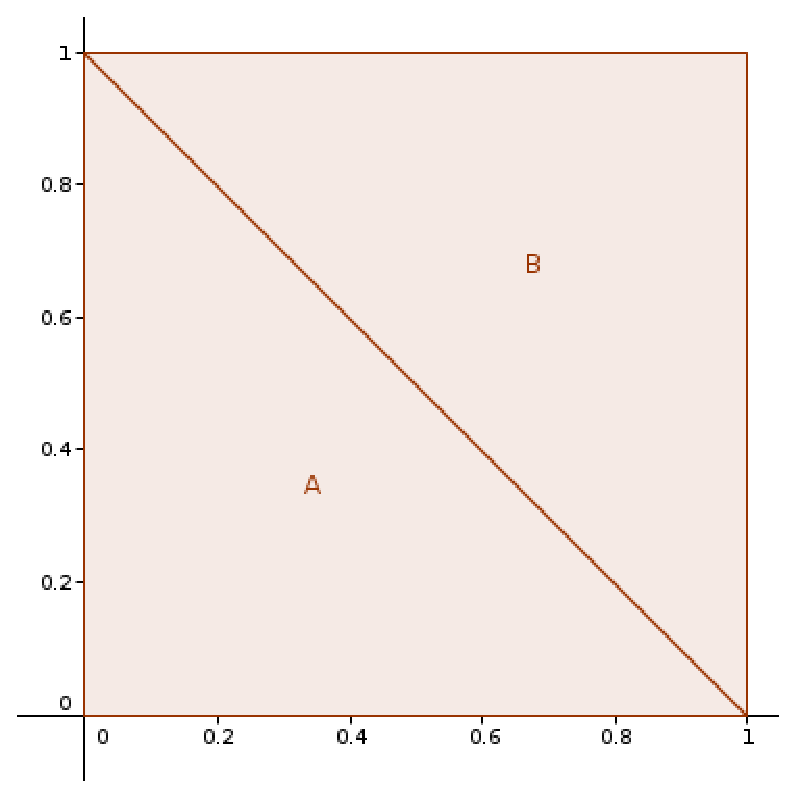
\includegraphics[scale=0.4]{Ej3paso1.eps}
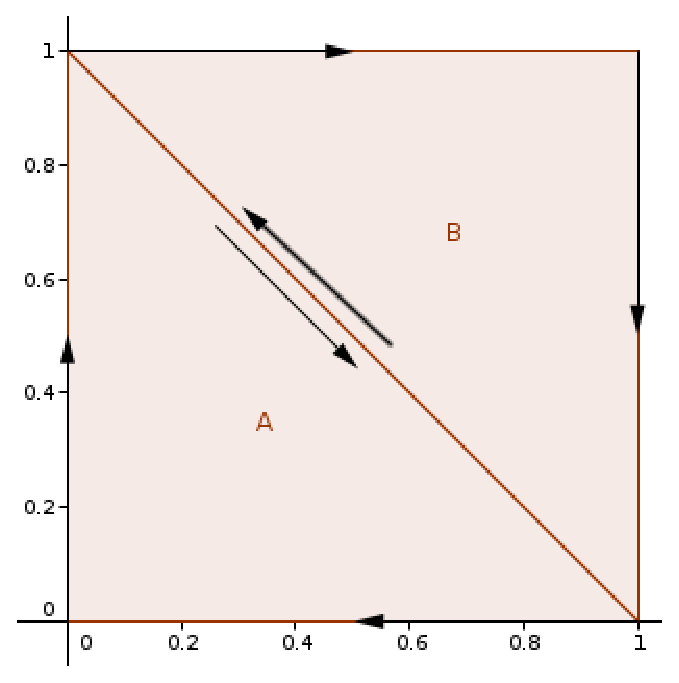
\includegraphics[scale=0.475]{Ej3paso2.eps}
\caption{$C$ queda dividido en dos triángulos, $A$ y $B$, a los cuales asignamos orientaciones contrarias orientando los bordes en direcciones opuestas.}
\end{figure}

Asignaremos a los segmentos $[(0,t)]$ y $[(1,t)]$ orientaciones contrarias. Estas orientaciones nos permiten orientar de forma única $A$ y $B$ a partir de sus bordes (ver figura 1).
\\

Definimos los 2-símplices singulares
\[\begin{array}{cccc}
\alpha:& \sigma_2 &\longrightarrow &C\\
            &(t_0,t_1,t_2)&\mapsto             &[(t_0,t_1)]
\end{array}\]

\[\begin{array}{cccc}\beta:& \sigma_2 &\longrightarrow &C\\
            &(t_0,t_1,t_2)&\mapsto             &[(t_0+t_1,t_0+t_2)]
\end{array}\]

Teniendo en cuenta que $(t,0)\sim (t,1)$ para todo $t \in [0,1]$,
\begin{align*}
\partial(\beta-\alpha)&(t_0,t_1)=\\
             &=[(t_0,t_1)]-[(t_0,t_1)]-[(t_0,1)]+[(1,t_0)]-[(0,t_0)]+[(t_0,0)]=\\
             &=[(1,t_0)]-[(0,t_0)]+[(t_0,0)]-[(t_0,0)]=\\
             &=[(1,t_0)]-[(0,t_0)]
\end{align*}

Dado que $F$ es una aplicación continua, induce una aplicación de cadenas $F_\#: S_*(C) \rightarrow S_*(X)$.
\begin{align*}
\partial [F_\#(\gamma-\alpha)](t_0,t_1)=&F_\#[\partial(\beta- \alpha)](t_0,t_1)=\\
                                       =&F(1,t_0)-F(0,t_0)=f(t_0)-g(t_0)
\end{align*}

Dado que $F_\#(\gamma-\alpha)=F_\#(\gamma)-F_\#(\alpha)$ es un 2-símplice singular de $X$, se deduce que $$f-g \in B_1(X) \iff f+B_1(X)=g+B_1(X)$$ Por tanto, $f$ y $g$ son caminos homólogos.\end{proof}

\section{Grupo de homología de $S^1$}
Sean $U=S^1-\{(1,0)\}$ y $V=S^1-\{(-1,0)\}$. Tenemos que $U\cap V$ es la unión disjunta de dos arcos de circunferencia, $C_1$ y $C_2$, que son conjuntos arcoconexos. Aplicando la proposición \ref{SumaDirArco}, se tiene que $$H_n(U\cap V) \cong H_n(C_1)\oplus H_n(C_2)$$ para todo $n \geq 0$.
\\

Dado que $C_1$ y $C_2$ son curvas cerradas y simples, son homeomorfas a un intervalo abierto $I \subset \mbR$ arbitrario, por lo que $$H_n(C_1) \cong H_n(I) \cong H_n(C_2)$$ Pero claro, los intervalos son conjuntos convexos, por lo que se deduce de la proposición \ref{Convexo} que $H_n(I)=0$ para todo $n > 0$ y $H_0(I)\cong\mb{Z}$.
\\

Combinando toda esta información, concluimos que $$H_n(U\cap V) \cong H_n(C_1)\oplus H_n(C_2) \cong H_n(I)^2 \cong \begin{cases}\mb{Z}^2 &\mbox{ si } n =0 \\ 0 &\mbox{ si no}\end{cases}$$

Por otro lado, $U$ y $V$ también son homeomorfos a un intervalo abierto de la recta real, por lo que podemos aplicar el mismo razonamiento para concluir que $$H_n(U) \cong 0 \cong H_n(V)\quad (n > 0)$$ y que $H_0(V) \cong \mb{Z} \cong H_0(U)$.
\\

Consideremos el siguiente tramo de la sucesión de Mayer-Vietoris asociada a este recubrimiento, donde las flechas verticales indican isomorfismos.
\[\begin{array}{ccccc}
H_1(U)\oplus H_1(V)	&\xrightarrow{h_1}	&H_1(S^1)		&\xrightarrow{\Delta_1}&H_0(U \cap V)\\
\downarrow			&					&\downarrow	&					&\downarrow\\
0			&\rightarrow			&H_1(S^1)		&\rightarrow			&\mb{Z}^2
\end{array}\]

Como la sucesión es exacta, $\im h_1=0$, luego $\ker_1 \Delta = \im h_1=0$, de forma que $\Delta$ es un monomorfismo. Se sigue que $$H_1(S^1)\cong \im \Delta = \ker g_1 \leq H_0(U\cap V)\cong \mb{Z}^2$$

Como $H_1(S^1) \cong \ker g_*$, podemos calcular dicho grupo estudiando cómo se comporta el homomorfismo $g_*$.
\\

Sea $w \in Z_0(U \cap V)$ y $[w]$ su clase módulo $B_0(U \cap V)$. Existirán $x,y \in U \cap V$, uno en cada componente conexa, y $a,b \in \mb{Z}$ tales que $$[w]=[ax+by]$$ Considérense las aplicaciones inclusión $$i_*: H_0(U \cap V) \hookrightarrow H_0(U); \quad j_*: H_0(U \cap V) \hookrightarrow H_0(V)$$ Si $[w] \in \ker g_*$, se tiene que
$$0=g_*([w])=(i_*([w]),-j_*([w])) \iff
\begin{cases}
i_*([w])=0\\
j_*([w])=0
\end{cases}$$
Pero $i_*([w]) \in H_0(U)$, por lo que $i_*([x])$ es homólogo a $i_*([y])$ y $$0=i_*([ax+by])=i_*([ax+bx])=(a+b)i_*([x]) \iff a+b=0$$ De aquí se tiene entonces que los elementos de $\ker g_*$ son de la forma $[ax-ay]$ con $a \in \mb{Z}$. Por tanto, $$H_1(S^1) =\ker g_*=\la[x-y]\ra \cong \mb{Z}$$

Sea $n > 1$. Se tiene la sucesión exacta
\[\begin{array}{ccccc}
H_n(U)\oplus H_n(V)	&\xrightarrow{h_n}	&H_n(S^1)		&\xrightarrow{\Delta_n}&H_{n-1}(U \cap V)\\
\downarrow	&					&\downarrow&&\downarrow\\
0			&\rightarrow			&H_n(S^1)		&\rightarrow			&0
\end{array}\]

Como esta sucesión es exacta, $\ker \Delta_n=\im h_n=0$. Por el primer teorema de isomorfia, se tiene que $$H_n(S^1) \cong \frac{H_n(S^1)}{0}=\frac{H_n(S^1)}{\ker \Delta_n} \cong \im \Delta_n=0$$

\begin{teo}\label{HomoS1}
\[\begin{array}{ccc}
H_n(S^1)\cong
\begin{cases}
\mb{Z}&\mbox{ si }n < 2\\
0     &\mbox{ si }n \geq 2
\end{cases}
&\implies&
\beta_n(S^1)=
\begin{cases}
1 &\mbox{ si }n < 2\\
0 &\mbox{ si }n \geq 2
\end{cases}
\end{array}\]
$$\chi(S^1)=\beta_0(S^1)-\beta_1(S^1)=1-1=0$$
\end{teo}

\begin{ejem}
Vamos a continuar con el ejemplo \ref{Deformacion}: habíamos visto que $S^1$ es una deformación de $D^2$ y un retracto de $D^2-\{(0,0)\}$. En general, esto es válido para cualquier $p \in int(D^2)$, no sólo para $p=(0,0)$, pero $S^1$ \textbf{no} es un retracto de todo $D^2$.
\\

Veámoslo: supongamos que existe un retracto $r: D^2 \longrightarrow S^1$. Como vimos en el tema anterior, todo retracto induce un epimorfismo $$r_*: H_1(D^2) \longrightarrow H_1(S^1)$$ en homología.
\\

$H_1(D^2)$ es 0 porque $D^2$ es un conjunto convexo, y acabamos de ver que $H_1(S^1)$ tiene rango 1. Dado que $r_*$ es un epimorfismo, si llamamos $\alpha$ al generador de $H_1(S^1)$, existirá un $b \in H_1(D^2)$ tal que $$r_*(b)=\alpha$$

Dado que $b \in H_1(D^2)=0$, $b=0$, por lo que $\alpha=r_*(b)=0$. Pero eso es imposible porque $\alpha$ es el generador de un grupo no trivial.
\\

Por tanto, no existen retracciones de $D^2$ en $S^1$.\qed
\end{ejem}

\section{Grupo de homología de la figura ocho}
La figura ocho se define como la curva formada por dos circunferencias tangentes, es decir: $$8:=C(-1,1)\cup C(1,1)$$

Considérese la aplicación $$\funcio{f}{[0,2\pi]}{\mb{C}}{t}{e^{it}}$$ Podemos tomar el recubrimiento formado por los abiertos $U=8-\{(2,0)\}$ y $V=f([-\pi/2,\pi/2])$.
\\

\begin{figure}[h]
\centering
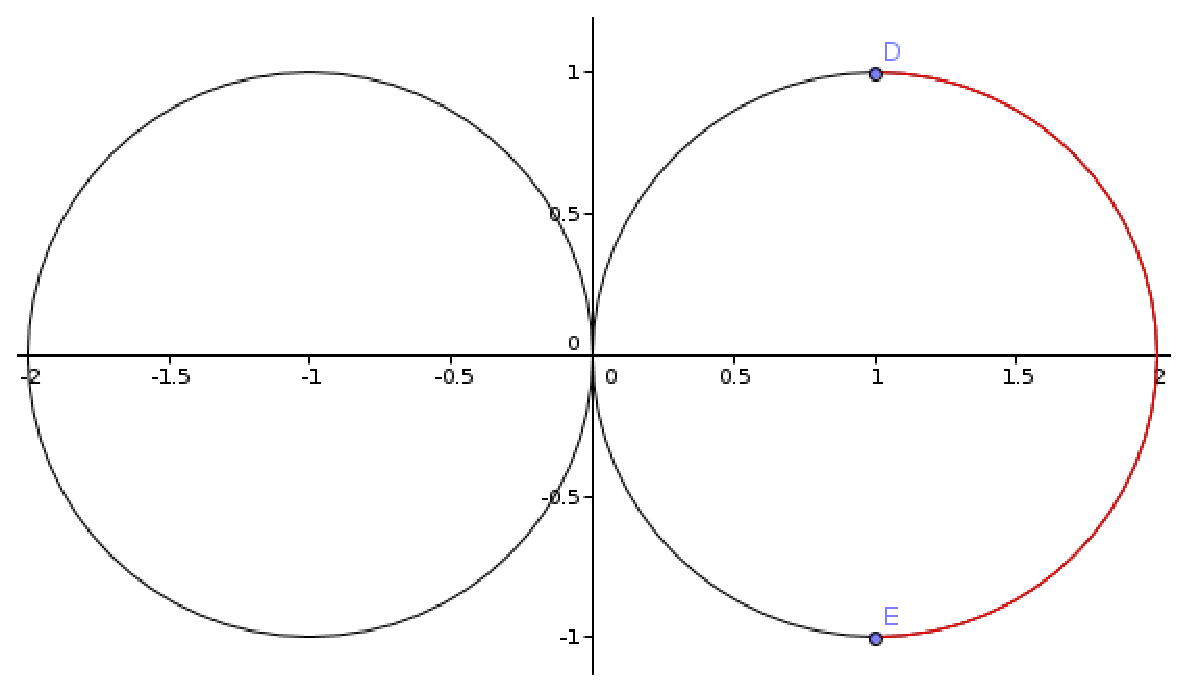
\includegraphics[scale=0.6]{Fig8Plano.eps}
\caption{Figura ocho. El conjunto $U$ será la curva negra, mientras que el conjunto $V$ será la curva roja que une los puntos $D$ y $E$.}
\end{figure}

$C(-1,1)\cong S^1$ es un retracto por deformación fuerte de $U$, mientras que $V \cong I$, que es un conjunto convexo. Por tanto, se tiene que $$H_*(U)=H_*(S^1); \quad H_*(V)=H_*(I)=H_*(\{0\})$$ Por otro lado, $U \cap V$ es la unión disjunta de dos segmentos, por lo que $$H*(U \cap V)\cong H_*(I)^2 \cong H_*(0)^2$$

Para $n > 1$, se tiene la sucesión exacta corta
\[\begin{array}{ccccccc}
H_n(U \cap V)	&\xrightarrow{g_*}	&H_n(U)\oplus H_n(V)	&\xrightarrow{h_*}	&H_n(8)		&\xrightarrow{\Delta}&H_{n-1}(U \cap V)\\
\downarrow		&					&\downarrow			&					&\downarrow	&					&\downarrow\\
0		&\rightarrow			&0			&\rightarrow			&H_n(8)		&\rightarrow			&0
\end{array}\]
donde las flechas verticales indican isomorfismos.
\\

Por exactitud, se tiene que
$$0=\im h_*\cong \frac{H_n(8)}{\ker h_*}=\frac{H_n(8)}{\im g_*}\cong H_n(8)$$

Consideremos ahora el sigueinte tramo de la sucesión de Mayer-Vietoris asociada a este recubrimiento, donde las flechas verticales indican isomorfismos.
\[\begin{array}{ccccccc}
H_1(U \cap V)	&\xrightarrow{g_1}	&H_1(U)\oplus H_1(V)	&\xrightarrow{h_1}	&H_1(8)		&\xrightarrow{\Delta_1}&H_0(U \cap v)\\
\downarrow		&					&\downarrow			&					&\downarrow	&					&\downarrow\\
0		&\rightarrow			&\mb{Z}			&\rightarrow			&H_1(8)		&\rightarrow			&\mb{Z}^2
\end{array}\]

Por exactitud, se tiene que $0=\im g_1=\ker h_1$, luego $$\mb{Z} \cong \frac{\mb{Z}^2}{\ker h_1} \cong \im h_1 =\ker \Delta_1$$

Consideremos ahora el sigueinte tramo de la sucesión de Mayer-Vietoris asociada a este recubrimiento, donde las flechas verticales indican isomorfismos.
\[\begin{array}{ccccccc}
H_0(U \cap V)	&\xrightarrow{g_0}	&H_0(U)\oplus H_0(V)	&\xrightarrow{h_0}	&H_0(8)		&\rightarrow&0\\
\downarrow		&					&\downarrow			&					&\downarrow	&					&\downarrow\\
\mb{Z}^2		&\rightarrow			&\mb{Z}^2			&\rightarrow			&\mb{Z}		&\rightarrow			&0
\end{array}\]

Por exactitud, se tiene que
\ecua{\label{Homo1Fig8}\frac{H_1(8)}{\ker \Delta_1} \cong \im \Delta_1 =\ker g_0}
$$\mb{Z} \cong \im h_0 \cong \frac{\mb{Z}^2}{\ker h_0} \implies \mb{Z} \cong \ker h_0 = \im g_0 \cong \frac{\mb{Z}^2}{\ker g_0}$$ de donde se sigue que $\ker g_0\cong \mb{Z}$.
\\

Aplicando este hecho a (\ref{Homo1Fig8}), concluimos que $$\mb{Z} \cong \frac{H_1(8)}{\mb{Z}} \quad\therefore\quad H_1(8) \cong \mb{Z}^2$$

\begin{teo}\label{HomoOcho}
\[\begin{array}{ccc}
H_n(8)\cong
\begin{cases}
\mb{Z}		&\mbox{ si }n =0\\
\mb{Z}^2	&\mbox{ si }n =1\\
0     &\mbox{ si }n \geq 2
\end{cases}
&\implies&
\beta_n(8)=
\begin{cases}
1 &\mbox{ si }n = 0\\
2 &\mbox{ si }n = 1\\
0 &\mbox{ si }n \geq 2
\end{cases}
\end{array}\]
$$\chi(8)=\beta_0(8)-\beta_1(8)=1-2=-1$$
\end{teo}

\subsection{La rosa del topólogo}
La figura ocho se puede construir de la forma siguiente: sea $p \in \mbR^2$ un punto e $I_1=[a_1,b_1], I_2=[a_2,b_2] \subset \mbR$ dos intervalos acotados. Si \[R=\partial I_1\cup \partial I_2\cup \{p\}\] se tiene que la figura ocho antes descrita se puede representar como \[\frac{I_1\sqcup\{p\}\sqcup I_2}{R}\]

Podemos extender esta construcción para añadir tantos lóbulos como queramos, de forma que conseguimos una figura llamada \textbf{rosa} o \textbf{buqué}.
\\

Sea $n > 0$ e $I_1=[a_1,b_1], \dots, I_n=[a_n,b_n] \subset \mbR$ una familia de intervalos acotados. Se define la rosa de $n$ pétalos ($B_n$) de la forma siguiente:
\[J_1=I_1\sqcup \{p\} \quad\land\quad R_1=\{p\}\cup \partial I_1 \implies B_1=\frac{J_1}{R_1}\cong S^1\]
\[J_2=J_1 \sqcup I_2 \quad\land\quad R_2=R_1 \cup \partial I_2 \implies B_2=\frac{J_2}{R_2} \cong 8\]
Esto crea una recurrencia que nos lleva a la definición de $B_n$, la rosa de $n$ pétalos: \[J_n=J_{n-1}\sqcup I_n \quad\land\quad R_n=R_{n-1}\cup \partial I_n \implies B_n=\frac{J_n}{R_n}\]

Hasta ahora, sabemos que
\[H_n(B_1)\cong
\begin{cases}
\mb{Z}		&\mbox{ si }n =0\\
\mb{Z}	&\mbox{ si }n =1\\
0     &\mbox{ si }n \geq 2
\end{cases}
\quad
H_n(B_2)\cong
\begin{cases}
\mb{Z}		&\mbox{ si }n =0\\
\mb{Z}^2	&\mbox{ si }n =1\\
0     &\mbox{ si }n \geq 2
\end{cases}
\]

Uno podría aventurarse a decir que cada pétalo de $B_p$ añade un nuevo generador al orden de homología de orden 1, y que el grupo de homología de orden $n > 1$ siempre es cero. Dado que lo tenemos confirmado para $p=1$ y $p=2$, podemos conjeturar cuál será el grupo de homología de orden 1 de $B_p$ para cualquier $p$.
\\

\textbf{Hipótesis de inducción:} Dado un $p$ natural,
\[\begin{array}{ccc}
H_n(B_p)\cong
\begin{cases}
\mb{Z}		&\mbox{ si }n =0\\
\mb{Z}^p	&\mbox{ si }n =1\\
0     &\mbox{ si }n \geq 2
\end{cases}
&\implies&
\beta_n(B_p)=
\begin{cases}
1 &\mbox{ si }n = 0\\
p &\mbox{ si }n = 1\\
0 &\mbox{ si }n \geq 2
\end{cases}
\end{array}\]

Consideremos entonces la rosa de $p+1$ pétalos, $B=B_{p+1}$. Definimos el recubrimiento de $B$ de la forma siguiente: tomamos un intervalo $I_j$ de los que conforman la rosa y dos puntos $p < q \in \mbox{int}(I_j)$. Se definen entonces los conjuntos $U=I_j$ y $V=B-[p,q]$.

\begin{figure}[h]
\centering
\includegraphics[scale=0.8]{Figures/Rosa}
\caption{Ejemplo de recubrimiento de la rosa de $p$ pétalos para $p=1,\dots,5$.}
\end{figure}

Observar que el espacio puntual $\{\star\}$ es un RDF de $U$, $B_p$ es un RDF de $V$ y que $\{\star\}\sqcup\{\star\}$ un RDF de $U\cap V$.
\\

Para $n > 1$, se tiene la sucesión exacta corta
\[\begin{array}{ccccccc}
H_n(U \cap V)	&\xrightarrow{g_*}	&H_n(U)\oplus H_n(V)	&\xrightarrow{h_*}	&H_n(B)		&\xrightarrow{\Delta}&H_{n-1}(U \cap V)\\
\downarrow		&					&\downarrow			&					&\downarrow	&					&\downarrow\\
0		&\rightarrow			&0			&\rightarrow			&H_n(B)		&\rightarrow			&0
\end{array}\]

Por exactitud, se tiene que $\ker \Delta=0$ y $\im \Delta=0=H_{n-1}(U\cap V)$, por lo que $\Delta$ es un isomorfismo. Se sigue que $$H_n(B) \cong H_{n-1}(U\cap V)=0$$

Consideremos ahora el sigueinte tramo de la sucesión de Mayer-Vietoris asociada a este recubrimiento:
\[\begin{array}{ccccccc}
H_0(U \cap V)	&\xrightarrow{g_0}	&H_0(U)\oplus H_0(V)	&\xrightarrow{h_0}	&H_0(B)		&\rightarrow&0\\
\downarrow		&					&\downarrow			&					&\downarrow	&					&\downarrow\\
\mb{Z}^2		&\rightarrow			&\mb{Z}^2			&\rightarrow			&\mb{Z}		&\rightarrow			&0
\end{array}\]

Por exactitud, se tiene que $\im h_0 \cong \mb{Z}$, por lo que $\im g_0=\ker h_0 \cong \mb{Z}$. De aquí se sigue que $\im \Delta_1=\ker g_0 \cong \mb{Z}$.
\\

Consideremos ahora el sigueinte tramo de la sucesión de Mayer-Vietoris asociada a este recubrimiento.
\[\begin{array}{ccccccc}
H_1(U \cap V)	&\xrightarrow{g_1}	&H_1(U)\oplus H_1(V)	&\xrightarrow{h_1}	&H_1(B)		&\xrightarrow{\Delta_1}&H_0(U \cap v)\\
\downarrow		&					&\downarrow			&					&\downarrow	&					&\downarrow\\
0		&\rightarrow			&\mb{Z}^p			&\rightarrow			&	H_1(B)	&\rightarrow			&\mb{Z}^2
\end{array}\]

Por exactitud, se tiene que $\ker h_1=\im g_1=0$, por lo que $\ker \Delta_1=\im h_1\cong \mb{Z}^p$. Como ya sabemos que $\im \Delta_1 \cong \mb{Z}$, se sigue que $$\frac{H_1(B)}{\mb{Z}^p} \cong \frac{H_1(B)}{\ker \Delta_1} \cong \im \Delta_1 \cong \mb{Z} \implies H_1(B)\cong \mb{Z}^{p+1}$$

Esto confirma nuestra conjetura. Además, $$\chi(B_p)=\beta_0(B_p)-\beta_1(B_p)=1-p$$

\section{Grupo de homología del toro}
El \textbf{toro paramétrico} se define como la superficie de ecuación implícita $$z^2+\left(R-\sqrt{x^2+y^2}\right)^2=r^2; \quad 0 < r < R$$ Podemos considerar un recubrimiento del toro paramétrico formado por dos cilindros que se solapan, $U$ y $V$, como los mostrados en la figura \ref{ToroUV}.
\\

\begin{figure}[h]
\centering
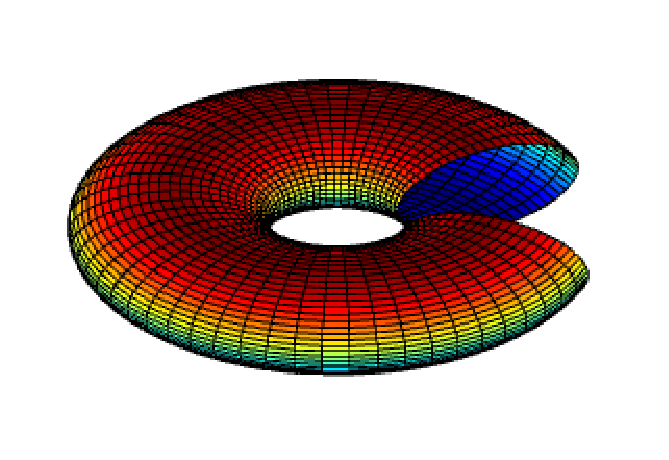
\includegraphics[scale=0.6]{ToroU.eps}
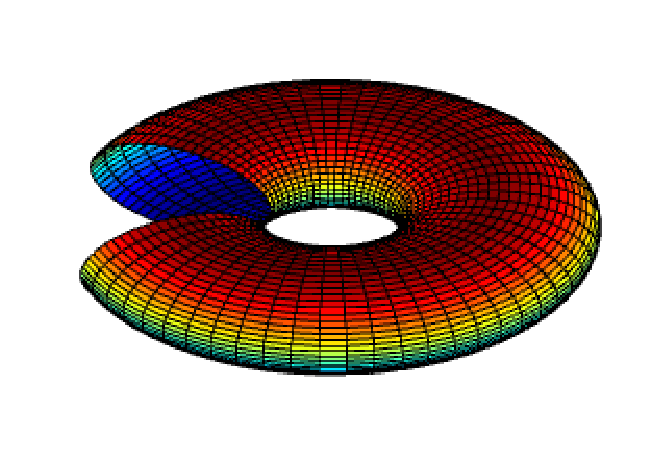
\includegraphics[scale=0.6]{ToroV.eps}
\caption{\label{ToroUV} Las figuras $U$ y $V$. Notar que $S^1$ es un retracto por deformación fuerte de ambas figuras.}
\end{figure}

Dado que $S^1$ es un retracto por deformación fuerte de $U$ y de $V$, se tiene que $$H_*(U) \cong H_*(S^1)\cong H_*(V)$$

Por otro lado, $U\cap V$ posee dos arcocomponentes, $C_1$ y $C_2$, por lo que la proposición \ref{SumaDirArco} nos dice que$ H_*(U\cap V) \cong H_*(C_1)\oplus H_*(C_2)$. Como $S^1$ es un retracto por deformación fuerte de $C_1$ y de $C_2$, se sigue que $$H_*(C_1)\oplus H_*(C_2) \cong H_*(S^1)\oplus H_*(S^1)\cong H_*(S^1)^2$$

Sea $n > 2$. Considérese la siguiente sucesión exacta, donde las flechas verticales indican isomorfismos.

\[\begin{array}{ccccccc}
H_n(U \cap V)	&\xrightarrow{g_*}	&H_n(U)\oplus H_n(V)	&\xrightarrow{h_*}	& H_n(T)		&\xrightarrow{\Delta}&H_{n-1}(U \cap v)\\
\downarrow		&					&\downarrow			&					&\downarrow	&					&\downarrow\\
0				&\rightarrow			&0					&\rightarrow			&H_n(T)		&\rightarrow			&0
\end{array}\]

Dado que esta sucesión es exacta, podemos afirmar que $\ker \Delta=\im h_*=0$ y $\im \Delta \leq 0$, por lo que $$H_n(T) \cong \frac{H_n(T)}{\ker \Delta} \cong \im \Delta \leq 0 \implies H_n(T)=0$$

\noindent\textbf{Cálculo de $H_2(T)$}
\\
Considérese la siguiente sucesión exacta, donde las flechas verticales indican isomorfismos.
\[\begin{array}{ccccccc}
H_0(U \cap V)	&\xrightarrow{g_0}	&H_0(U)\oplus H_0(V)	&\xrightarrow{h_0}	&H_0(T)		&\xrightarrow{f}&0\\
\downarrow		&					&\downarrow			&					&\downarrow	&					&\downarrow\\
\mb{Z}^2			&\rightarrow			&\mb{Z}^2			&\rightarrow			&\mb{Z}		&\rightarrow			&0
\end{array}\]

Dado que esta sucesión es exacta, podemos afirmar que $\im h_0=\ker f \cong \mb{Z}$ y $\im g_0=\ker h_0\cong \mb{Z}$, luego $$\frac{\mb{Z}^2}{\ker h_0} \cong \im h_0 \cong \mb{Z} \implies \ker h_0\cong\mb{Z}$$ $$\frac{\mb{Z}^2}{\ker g_0} \cong \im g_0 \cong \mb{Z} \implies \ker g_0\cong\mb{Z}$$

Considérese el siguiente tramo de la sucesión de Mayer-Vietoris asociada a este recubrimiento, donde las flechas verticales indican isomorfismos.
\[\begin{array}{ccccccc}
H_1(U \cap V)	&\xrightarrow{g_1}	&H_1(U)\oplus H_1(V)	&\xrightarrow{h_1}	&H_1(T)		&\xrightarrow{\Delta_1}&H_0(U \cap V)\\
\downarrow		&					&\downarrow			&					&\downarrow	&					&\downarrow\\
\mb{Z}^2			&\rightarrow			&\mb{Z}^2			&\rightarrow			&H_1(T)		&\rightarrow			&\mb{Z}^2
\end{array}\]

Dado que la sucesión es exacta,
$$\frac{H_1(T)}{\ker \Delta_1}\cong \im \Delta_1=\ker g_0\cong \mb{Z}$$

Considérese el siguiente tramo de la sucesión de Mayer-Vietoris asociada a este recubrimiento, donde las flechas verticales indican isomorfismos.
\[\begin{array}{ccccccc}
H_2(U \cap V)	&\xrightarrow{g_2}	&H_2(U)\oplus H_2(V)	&\xrightarrow{h_2}	& H_2(T)		&\xrightarrow{\Delta_2}&H_1(U \cap v)\\
\downarrow		&					&\downarrow			&					&\downarrow	&					&\downarrow\\
0				&\rightarrow			&0					&\rightarrow			&H_2(T)		&\rightarrow			&\mb{Z}^2
\end{array}\]

Dado que la sucesión es exacta,
$$H_2(T) \cong \frac{H_2(T)}{\im h_2}=\frac{H_2(T)}{\ker \Delta_2} \cong \im \Delta_2=\ker g_1$$

Recordemos cómo se define $g_*$: $$\funcio{g_*}{H_1(C_1\sqcup C_2)}{H_1(U)\oplus H_1(V)}{[c]}{([c],[-c])}$$ Sea $[c] \in \ker g_*$. Dado que $S^1$ es un retracto por deformación fuerte del cilindro, existen ciclos $x,y \in Z_1(S^1)$ tales que $$H_1(C_1\sqcup C_2)\cong H_1(S^1)\oplus H_1(S^1)=([x])_\mb{Z}\oplus ([y])_\mb{Z}$$ de forma que $c=\alpha x+\beta y$ para algunos $\alpha,\beta$ enteros.
\\

Considérense ahora las inclusiones $i: U \cap V \hookrightarrow U$ y $j: U \cap V \hookrightarrow V$. Se tiene que $$0=g_*([c])=([c],-[c])=(i_*[c],-j_*[c]) \iff \begin{cases}i_*([c])=0\\j_*([c])=0\end{cases}$$ Dado que $x$ e $y$ son símplices homólogos en $U$, $$i_*([c])=i_*([\alpha x+\beta y])=i_*([\alpha x+\beta x])=(\alpha+\beta)i_*([x])=0 \iff \alpha=-\beta$$ Se sigue que $$H_2(T)\cong \ker g_*=\{[\alpha x-\alpha y]: \alpha \in \mb{Z}\}=([x-y])_\mb{Z}\cong \mb{Z}$$

\noindent\textbf{Cálculo de $H_1(T)$}
\\
Considérese la siguiente relación de equivalencia sobre $I^2$: $$\forall s,t \in [0,1] \quad (s,0) \sim (s,1) \land (0,t) \sim (1,t)$$ El espacio cociente $T_C=I^2/\sim$ se denomina \textbf{toro llano}, y es homeomorfo al toro paramétrico. Si $p=(1/2,1/2)$, $I^2-\{p\}$ es deformable en $\partial(I^2)$, por lo que $\partial(I^2)$ es un retracto por deformación de $I^2-\{p\}$.
\\

Se puede definir una retracción que sea compatible con la relación de equivalencia $\sim$, de forma que $\partial T_C$ es un retracto por deformación del toro llano. Esta figura es homeomorfa a la figura ocho, como puede verse en la figura \ref{fig8}.
\\

\begin{figure}[h]
\centering
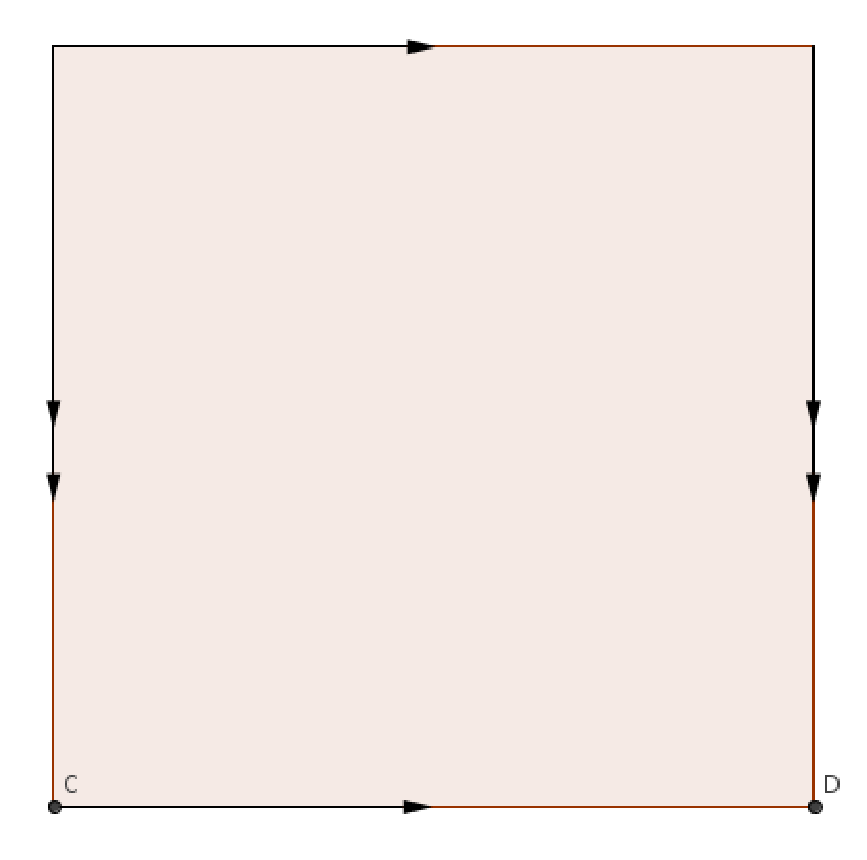
\includegraphics[scale=0.4]{Clifford.eps}\hspace{2cm}
\includegraphics[scale=0.55]{FiguraOcho.eps}
\caption{\label{fig8}Izquierda: toro llano. Derecha: figura ocho proyectada sobre el toro paramétrico.}
\end{figure}

Sea ahora $V=B(p;1/4)$. Se tiene que $V \subset I^2$ y $V\cap\partial (I^2)=\emptyset$, de forma que $V$ y $U=T_C-\{p\}$ forman un recubrimiento del toro llano. Ahora bien, $U \cap V$ es una corona circular, por lo que $S^1$ es un retracto por deformación fuerte de $U \cap V$. Así, se tiene que $$H_*(T-\{p\}) \cong H_*(8); \quad H_*(V) \cong H_*(\{p\}); \quad H_*(U \cap v) \cong H_*(S^1)$$

Considérese el siguiente tramo de la sucesión de Mayer-Vietoris asociada a este recubrimiento, donde las flechas verticales indican isomorfismos.
\[\begin{array}{ccccccc}
H_2(U \cap V)	&\xrightarrow{g_2}	&H_2(U)\oplus H_2(V)	&\xrightarrow{h_2}	& H_2(T)		&\xrightarrow{\Delta_2}&H_1(U \cap V)\\
\downarrow		&					&\downarrow			&					&\downarrow	&					&\downarrow\\
0				&\rightarrow			&0					&\rightarrow			&\mb{Z}		&\rightarrow			&\mb{Z}
\end{array}\]

Dado que la sucesión es exacta, se tiene que $0=\im h_2=\ker \Delta_2$, luego $$\im \Delta_2\cong \frac{H_2(T)}{\ker \Delta_2} \cong \mb{Z}$$

Considérese el siguiente tramo de la sucesión de Mayer-Vietoris asociada a este recubrimiento, donde las flechas verticales indican isomorfismos.
\[\begin{array}{ccccccc}
H_1(U \cap V)	&\xrightarrow{g_1}	&H_1(U)\oplus H_1(V)	&\xrightarrow{h_1}	&H_1(T)		&\xrightarrow{\Delta_1}&H_0(U \cap V)\\
\downarrow		&					&\downarrow			&					&\downarrow	&					&\downarrow\\
\mb{Z}		&\rightarrow			&\mb{Z}^2			&\rightarrow			&H_1(T)		&\rightarrow			&\mb{Z}
\end{array}\]

Dado que la sucesión es exacta, se tiene que
$\mb{Z} \cong \im \Delta_2 =\ker g_1$, luego $$0=\frac{\mb{Z}}{\ker g_1}\cong \im g_1=\ker h_1 \implies \mb{Z}\cong \frac{\mb{Z}}{\ker h_1}\cong \im h_1=\ker \Delta_1$$ De aquí se sigue que $\im \Delta_1 \cong H_1(T)/\ker \Delta_1\cong H_1(T)/\mb{Z}$.
\\

Considérese el siguiente tramo de la sucesión de Mayer-Vietoris asociada a este recubrimiento, donde las flechas verticales indican isomorfismos.
\[\begin{array}{ccccccc}
H_0(U \cap V)	&\xrightarrow{g_0}	&H_0(U)\oplus H_0(V)	&\xrightarrow{h_0}	&H_0(T)		&\rightarrow&0\\
\downarrow		&					&\downarrow			&					&\downarrow	&					&\downarrow\\
\mb{Z}^2		&\rightarrow			&\mb{Z}^2			&\rightarrow			&\mb{Z}		&\rightarrow			&0
\end{array}\]

Ya tenemos toda la información necesaria para poder determinar $H_1(T)$: $$\mb{Z} \cong \im h_0 \cong \frac{\mb{Z}^2}{\ker h_0} \implies \ker h_0 \cong \mb{Z}$$
$$\mb{Z} \cong \ker h_0 =\im g_0 \cong \frac{\mb{Z}^2}{\ker g_0} \implies \ker g_0\cong \mb{Z}$$
$$\mb{Z} \cong \ker g_0 =\im \Delta_1 \cong \frac{H_1(T)}{\mb{Z}} \therefore H_1(T)\cong \mb{Z}^2$$

\begin{teo}\label{HomoToro}
\[\begin{array}{ccc}
H_n(T)=
\begin{cases}
\mb{Z}		&\mbox{ si }n =0,2\\
\mb{Z}^2	&\mbox{ si }n =1\\
0     &\mbox{ si }n > 2
\end{cases}
&\implies&
\beta_n(T)=
\begin{cases}
1 &\mbox{ si }n = 0,2\\
2 &\mbox{ si }n = 1\\
0 &\mbox{ si }n > 2
\end{cases}
\end{array}\]
Y esto nos lleva a un hecho que ya sabíamos: $$\chi(8)=\beta_0(T)-\beta_1(T)+\beta_2(T)=1-2+1=0$$
\end{teo}

\part{Espacios CW-complejos}
\chapter{Grupos de homología relativa}
\section{Qué aporta un subespacio a la homología}
Como vimos en el tema anterior, el grupo de homología de orden 1 de la rosa tiene tantos generadores como pétalos. De hecho, para ser más exactos, podemos hallar un representante de cada generador en uno de los pétalos.

\begin{figure}[h]
\centering
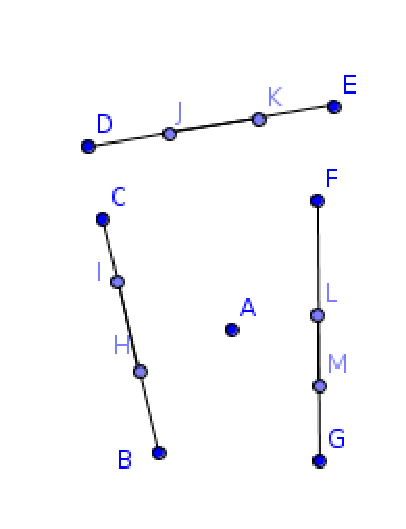
\includegraphics[scale=0.75]{Figures/Gen3Rosa.eps}
\caption{Representación de la rosa de 3 pétalos. Los segmentos $[I,H]$, $[J,K]$ y $[L,M]$ son los generadores de $H_1(B_3)$.}
\end{figure}

Esto parece decirnos que la acción de \textbf{añadir un pétalo} (que se llama \textbf{pegamento} o \textbf{adjunción}, como veremos en el capítulo siguiente) es la que provoca la aparición de nuevos generadores. No obstante, diferentes adjunciones provocan diferentes alteraciones:

\begin{enumerate}
\item Si pegamos sólo uno de los extremos del segmento a $B_p$ y dejamos el otro libre, $B_p$ es un retracto por deformación fuerte de la figura resultante, de forma que no aparecen nuevos generadores.
\item Si lo pegamos por ambos lados, aparece un pétalo nuevo y aparece un nuevo generador.
\end{enumerate}


Dado un espacio topológico $X$ y un subespacio $A \subseteq X$, el grupo de homología relativa estudia cómo $A$ está pegado con su complementario, $X-A$. Diremos que dos cadenas son \textit{iguales módulo $A$} si su diferencia es una cadena en $A$. En particular, tendremos que una cadena será un \textit{ciclo módulo $A$} si su borde está contenido en $A$.

\section{Complejo de cadenas cociente}
Diremos que un complejo de cadenas $(D,\partial')$ es un \textbf{subcomplejo} de $(C,\partial)$ si, dado un $p \in \mb{Z}$, se verifica que $$D_p \leq C_p \quad \land \quad \partial_p(D_p)\subseteq D_{p-1}$$

Un subcomplejo $(D,\partial)$ es \textbf{subcomplejo normal} de $(C,\partial)$ si $D$ es un subgrupo graduado normal de $C$.

\cuadro{Sea $(C,\partial)$ un complejo de cadenas y $(D,\partial')$ un subcomplejo de cadenas tal que $D \trianglelefteq C$. Se define el \textbf{complejo cociente} como el graduado $C/D$ dotado del operador borde siguiente: $$\funcio{Q_p}{C_p/D_p}{C_{p-1}/D_{p-1}}{c+D_p}{(\partial_p c)+D_{p-1}}$$}

Si $\pi: C \longrightarrow C/D$ es el epimorfismo canónico e $i: D \hookrightarrow C$ es la inclusión, se tiene que la sucesión $$0 \longrightarrow D \xrightarrow{i} C \xrightarrow{\pi} \frac{C}{D} \longrightarrow 0$$ es exacta. Según el teorema \ref{SucExacHomo}, si podemos hallar un homomorfismo de conexión $\Delta: H_*(C/D) \longrightarrow H_*(C)$ de grado -1, \ecua{\label{SECociente}H_n(D) \xrightarrow{i_*} H_n(C) \xrightarrow{\pi_*} H_n\left(\frac{C}{D}\right) \xrightarrow{\Delta} H_{n-1}(D)} será una sucesión exacta larga.
\\

\begin{nota}
Por cuestiones de economía en la notación, a la clase del elemento $c \in C_p$ en el grupo cociente $H_p(C/D)$ se la denotará como $[c+D_p]$ o simplemente $\la c\ra$. De esta forma, se reserva $[c]$ para la clase de $c$ en $H_*(C)$.
\end{nota}

Para construir el homomorfismo de conexión, sea $[c] \in Z_n(C/D)$. Se tiene que $$\partial_n c+D_n=0+D_{n-1} \implies \partial c \in D_{n-1}$$ Como $\partial(\partial c)=\partial^2c=0$, $\partial c \in Z_{n-1}(D)$, luego $\partial c+B_{n-1}(D) \in H_{n-1}(D)$. Definimos entonces el homomorfismo \ecua{\label{DeltaCociente}\funcio{\Delta_n}{H_n(C/D)}{H_{n-1}(D)}{c+D_n}{\partial c + B_{n-1}(D)}} de forma que $\Delta=\{\Delta_n: n \in \mb{Z}\}$ es un homomorfismo de conexión, haciendo que (\ref{SECociente}) sea una sucesión exacta larga.

\begin{lema}[Teorema de isomorfia para grupos graduados]\label{TTIGG}
Sea $C$ un complejo de cadenas y $E,D$ subcomplejos normales de $C$. Si $E$ es un subcomplejo de $D$, $$\frac{C}{D} \cong \frac{C/E}{D/E}$$
\end{lema}

\begin{proof}
Sea $p \in \mb{Z}$. Por definición de subcomplejo y subcomplejo normal, $D_p,E_p \trianglelefteq C_p$ y $E_p \leq D_p$. Por el tercer teorema de isomorfia, existe un isomorfismo $$f_p: \frac{C_p}{D_p} \longrightarrow \frac{C_p/E_p}{D_p/E_p}$$

Considérese entonces el homomorfismo graduado $f=\underset{p \in \mb{Z}}{\{f_p\}}$. Se tiene que $$f: \frac{C}{D} \longrightarrow \frac{C/E}{D/E}$$ es un isomorfismo graduado por ser una colección de isomorfismos. Por tanto, $C/D$ es isomorfo a $(C/E)/(D/E)$.
\end{proof}

Sea $C$ un complejo de cadenas y $E \leq D$ subcomplejos normales de $C$. Por el lema \ref{TTIGG}, existe un isomorfismo graduado $f: (C/E)/(D/E) \longrightarrow C/D$. Si ahora consideramos el epimorfismo canónico $\pi: C/E \longrightarrow (C/E)/(D/E)$, se tiene que $$\Pi: \frac{C}{E} \xrightarrow{\pi} \frac{C/E}{D/E} \xrightarrow{f} \frac{C}{D}$$ es un epimorfismo graduado entre $C/E$ y $C/D$. De aquí se obtiene la sucesión exacta corta $$0 \longrightarrow \frac{D}{E} \xrightarrow{i} \frac{C}{E} \xrightarrow{\Pi}\frac{C}{D} \longrightarrow 0$$

Dado un $n \in \mb{Z}$, sea $p_n: D_n \longrightarrow D_n/E_n$ el epimorfismo canónico. Se tiene que $p=\{p_n: n \in \mb{Z}\}$ induce un homomorfismo de grado 0 en homología, $$p_*: H_*(D) \longrightarrow H_*(D/E)$$ Si $\Delta: H_*(C/D) \longrightarrow H_*(D)$ es el homomorfismo graduado (\ref{DeltaCociente}), \ecua{\label{DeltaCPrima}\Delta': H_*(C/D) \xrightarrow{\Delta} H_*(D) \xrightarrow{p_*} H_*(D/E)} es un homomorfismo de conexión, por lo que el teorema \ref{SucExacHomo} nos dice que \ecua{\label{SECociente2}H_n\left(\frac{D}{E}\right) \xrightarrow{i_*}H_n\left(\frac{C}{E}\right)\xrightarrow{\Pi_*}H_n\left(\frac{C}{D}\right)\xrightarrow{\Delta'}H_{n-1}\left(\frac{D}{E}\right)} es una sucesión exacta larga.
\\

Sea $C'$ otro complejo de cadenas, con $E'\leq D'$ subcomplejos normales de $C'$. Considérese una aplicación de cadenas $g: C \longrightarrow C'$ tal que $g(D) \leq D'$ y $g(E) \leq E'$. Como acabamos de ver, se puede construir una sucesión exacta corta $$0 \longrightarrow \frac{D'}{E'} \longrightarrow \frac{C'}{E'} \longrightarrow \frac{C'}{D'} \longrightarrow 0$$ que induce una sucesión exacta larga en homología similar a (\ref{SECociente2}). Dado que $g$ es una aplicación de cadenas, podemos conectar ambas sucesiones exactas usando $g_*$: \ecua{\label{TNatural}\begin{array}{ccccccc}
H_n\left(\frac{D}{E}\right)&\xrightarrow{i_*}&H_n\left(\frac{C}{E}\right)&\xrightarrow{\Pi_*}&H_n\left(\frac{C}{D}\right)&\xrightarrow{\Delta'}&H_{n-1}\left(\frac{D}{E}\right)\\
%&&&&&&\\
g_*\downarrow&\circlearrowleft&g_*\downarrow&\circlearrowleft&g_*\downarrow&\circlearrowleft&g_*\downarrow\\
%&&&&&&\\
H_n\left(\frac{D'}{E'}\right)&\xrightarrow{\tilde{i}_*}&H_n\left(\frac{C'}{E'}\right)&\xrightarrow{\tilde{\Pi}_*}&H_n\left(\frac{C'}{D'}\right)&\xrightarrow{\tilde{\Delta}'}&H_{n-1}\left(\frac{D'}{E'}\right)
\end{array}}

Por cómo está construida la sucesión exacta (\ref{SECociente2}), se puede probar que cada uno de los cuadrados del diagrama (\ref{TNatural}) es conmutativo. Es decir, $$g_*\circ \tilde{i}_*=i_*\circ g_*; \quad g_*\circ \tilde{\Pi}_*=\Pi_*\circ g_*; \quad g_*\circ \tilde{\Delta}'=\Delta'\circ g_*$$ Se dice entonces que $g_*$ es una \textbf{transformación natural} o que cumple la \textbf{hipótesis de naturalidad}.
\\

\section{Homología singular relativa}
\cuadro{Un \textbf{par de espacios} es un par ordenado de la forma $(X,A)$, donde $X \in \topo$ y $A \subseteq X$ es un subespacio.}

Sea $(X,A)$ un par de espacios y $n > 0$. Dado un $c \in S_n(X)$, existen $n$-símplices singulares $$\phi_1,\dots,\phi_p: \sigma_n \longrightarrow X$$ y $\mu_1,\dots,\mu_p \in \mb{Z}$ tales que $$c=\sum^p_{i=1}\mu_i\phi_i$$ Si $\phi_i(\sigma_n) \subseteq A$ para cada $i=1,\dots,p$, se tiene entonces que $c \in S_n(A)$. De aquí se sigue que $S_n(A) \leq S_n(X)$.
\\

Por otro lado, dado un $i=0,\dots,n$, $$\partial_{(i)} \phi(\sigma_{n-1}) \subset \phi(\sigma_n) \subset A \implies \partial_{(i)}\phi \in S_{n-1}(A)$$ Dado que $$\partial_n \phi=\sum^n_{i=0}\partial_{(i)}\phi$$ se tiene que $\partial_n \phi \in S_{n-1}(A)$, por lo que $S_*(A)$ dotado del operador borde $\partial_A=\{\partial_n|_{S_n(A)}: n \in \mb{Z}\}$ es un subcomplejo de cadenas de $S_*(X)$.
\\

Se define el \textbf{complejo de cadenas singulares de $X$ módulo $A$} como el complejo cociente $$S_*(X,A):=\frac{S_*(X)}{S_*(A)}=\left\{\frac{S_n(X)}{S_n(A)}: n \in \mb{Z}\right\}$$ De la misma forma, se definen los grupos graduados $$Z_*(X,A):=\frac{Z_*(X)}{Z_*(A)}; \quad B_*(X,A):=\frac{B_*(X)}{B_*(A)}; \quad n \geq 0$$

\noindent\textbf{Una transformación que preserva el orden:}\\
Sean $X,Y$ espacios topológicos. Las relaciones binarias \textit{$X \leq Y$ si y sólo si $X$ es un subespacio topológico de $Y$} y \textit{$S_*(X) \leq S_*(Y)$ si sólo si $S_*(X)$ es un subcomplejo de cadenas de $S_*(X)$} son relaciones de orden, y acabamos de demostrar que $$X \leq Y \implies S_*(X) \leq S_*(Y)$$ Desde un punto de vista informal, podríamos decir que la transformación $X \mapsto S_*(X)$ \textit{preserva el orden}, porque transforma subespacios topológicos en subcomplejos de cadenas.

\cuadro{Sea $(X,A)$ un par de espacios. Se define el \textbf{grupo $n$-ésimo de homología singular relativa de $X$ módulo $A$} como $$H_n(X,A):=H_n(S_*(X,A))=\frac{Z_n(X,A)}{B_n(X,A)}$$}

\begin{ejem}\label{EjEsfera}
Sea $X=S^2$. Considérense las curvas $c,d \subset X$ mostradas en la figura \ref{FigEsfera}, y sea $A$ la componente conexa de $X-d$ que no contiene a la curva $c$.
\\

Usando el ejemplo \ref{CaminoCiclo}, $c$ forma un ciclo en $X$ por ser un lazo, por lo que $\partial_1 c=0$. Por cómo se define el operador borde del complejo de cadenas cociente, $$\partial_1(c+S_1(A))=\partial_1 c+S_1(A)=0+S_1(A)$$ por lo que $c$ forma un ciclo en $(X,A)$.
\\

Sea $e$ el arco de circunferencia que une las curvas $c$ y $d$ en $X$, y $\tilde{A}=A\cup d$. $e$ no es un ciclo en $X$ porque no es un lazo, y tampoco es un ciclo en $(X,\tilde{A})$. No obstante, sí es un ciclo en $(X,\tilde{A}\cup c)$. Notar que ambos extremos del camino $e$ caen en algún punto de $\tilde{A}\cup c$.
\end{ejem}

\begin{figure}[h]
\centering
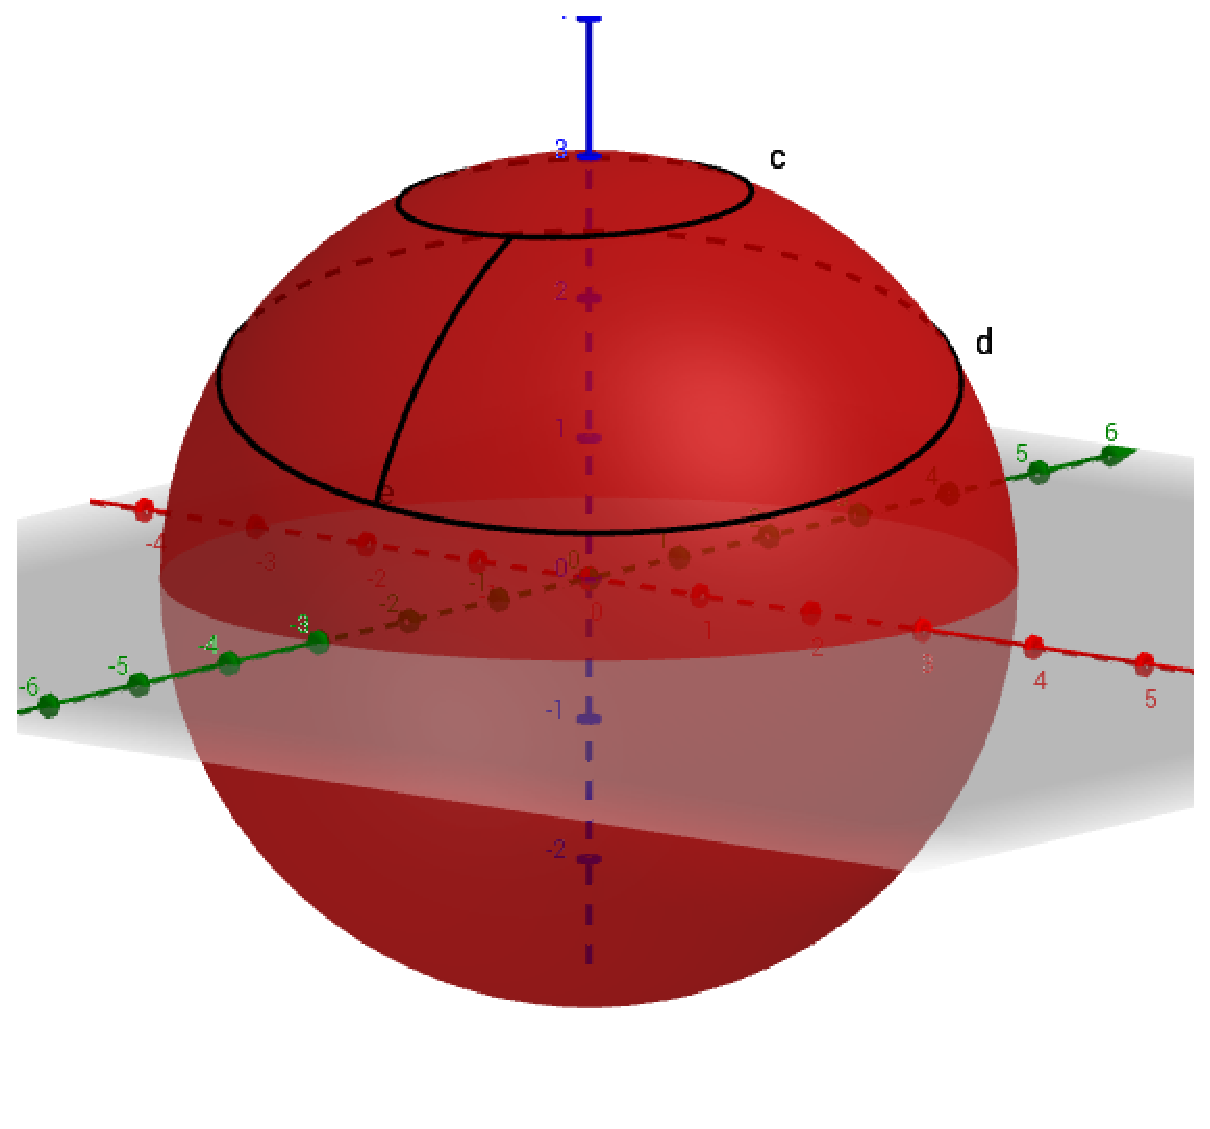
\includegraphics[scale=0.35]{Figures/EsferaParDEspais.eps}
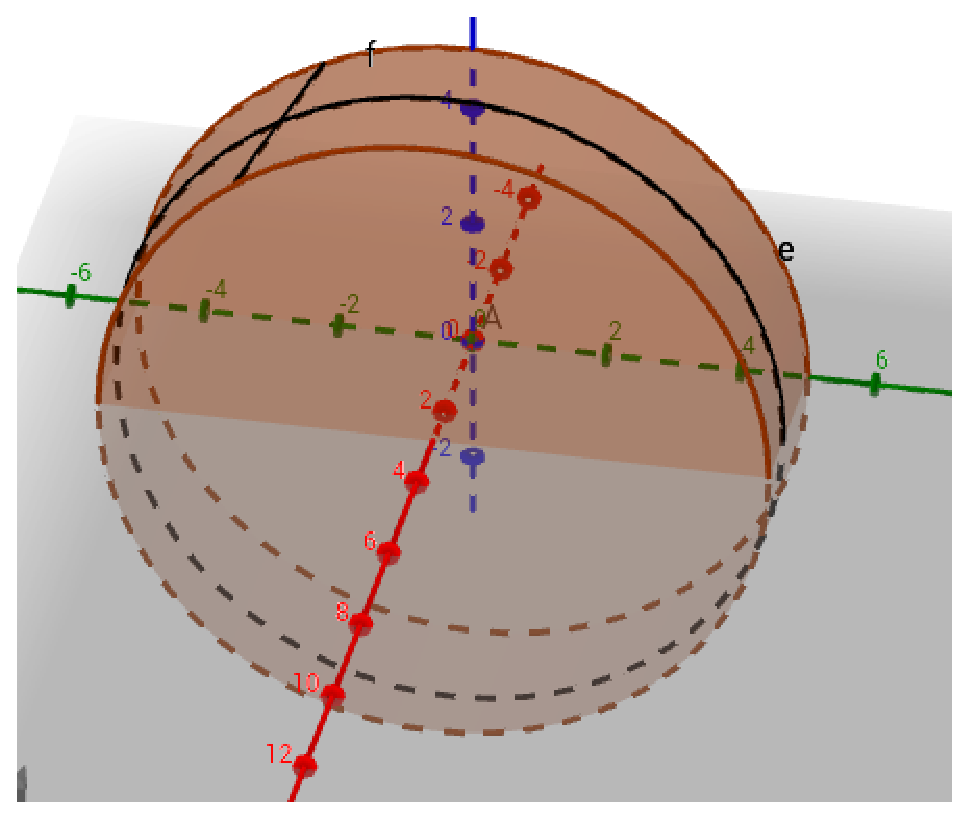
\includegraphics[scale=0.35]{Figures/CilParDEspais.eps}
\caption{\label{FigEsfera} Esfera del ejemplo \ref{EjEsfera} y cilindro de ejemplo \ref{EjCilindro}.}
\end{figure}

\begin{ejem}\label{EjCilindro}
Sea $X$ el cilindro con tapas mostrado en la figura \ref{FigEsfera}, y $A$ la unión de las dos tapas. Sobre $X$ dibujamos la circunferencia $e$ paralela a las anillas del cilindro y el segmento $f$, ambos mostrados en la figura \ref{FigEsfera}.
\\

Por un lado, la curva $e$ es un ciclo en $X$ por ser un lazo, y también lo es en $(X,A)$. Por otro lado, el segmento $f$ no es un ciclo en $X$, pero sí lo es en $(X,A)$. Observar que ambos extremos del camino $f$ recaen en algún punto de $A$.
\end{ejem}

\cuadro{Sea $(X,A)$ un par de espacios. Tomando $C=S_*(X)$ y $D=S_*(A)$ en la sucesión exacta (\ref{SECociente}), se obtiene la \textbf{sucesión exacta asociada al par $(X,A)$}: \ecua{\label{SEPares}H_n(A) \xrightarrow{i_*} H_n(X)\xrightarrow{\pi_*}H_n(X,A)\xrightarrow{\Delta}H_{n-1}(A)}}

\begin{prop}
$i_*$ es un isomorfismo si y sólo si $H_n(X,A)=0$ para todo $n \geq 0$.
\end{prop}

\cuadro{Una \textbf{tríada de espacios} es una terna $(X,A,B)$, donde $(X,A)$ y $(A,B)$ son pares de espacios.}

Sea $(X,A,B)$ una tríada de espacios. Tomando $D=S_*(A)$, $E=S_*(B)$ y $C=S_*(X)$ en (\ref{SECociente2}), se obtiene la sucesión exacta larga $$H_n(A,B) \stackrel{i_*}{\longrightarrow} H_n(X,B) \stackrel{j_*}\longrightarrow H_n(X,A) \stackrel{\Delta'}{\longrightarrow} H_{n-1}(A,B)$$ donde $i_*$ y $j_*$ son los homomorfismos inducidos en homología por las inclusiones $$i: S_*(A) \hookrightarrow S_*(X); \quad j: S_*(B) \hookrightarrow S_*(A)$$ y $\Delta'$ es la aplicación (\ref{DeltaCPrima}).
\\

Recordemos que el grupo libre generado por el vacío es el grupo trivial, de forma que $S_*(\emptyset)=0$. Esto nos permite establecer un isomorfismo natural entre $S_*(X)$ y $S_*(X,\emptyset)$: $$\funcio{f_n}{S_n(X)}{S_n(X,\emptyset)}{c}{c+S_n(\emptyset)}$$ De la misma forma, se tiene que $S_*(X,A,\emptyset) \cong S_*(X,A)$ y $S_*(X)\cong S_*(X,\emptyset,\emptyset)$.

\section{Aplicaciones entre pares}
\cuadro{Sean $(X,A)$ e $(Y,B)$ dos pares de espacios topológicos. Una \textbf{aplicación de pares} $$f: (X,A) \longrightarrow (Y,B)$$ es una aplicación continua $f: X \longrightarrow Y$ tal que $f(A) \subseteq B$.}

Si $\phi: \sigma_p \longrightarrow X$ es un símplice singular tal que $\phi(\sigma_p) \subset A$ y $$f: (X,A) \longrightarrow (Y,B)$$ es una aplicación de pares, se tiene que $(f\circ\phi)(\sigma_p) \subset B$, por lo que $f_\#(\phi)$ es un $p$-símplice singular de $B$. Dado que la elección de $\phi$ es arbitraria y los $p$-símplices singulares conforman una base de $S_*(A)$, se tiene que $$f_\#(S_*(A)) \subseteq S_*(B)$$ por lo que $f$ induce una aplicación de cadenas
\[\begin{array}{cccc}
f_\#:&S_*(X,A)&\longrightarrow&S_*(Y,B)\\
	 &c+S_*(A)&\longmapsto	 &f(c)+S_*(B)
\end{array}\]
que induce a su vez un homomorfismo entre los grupos de homología relativa,
\[\begin{array}{cccc}
f_*:&H_*(X,A)&\longrightarrow&H_*(Y,B)\\
	 &\la c\ra&\longmapsto	 &\la f(c)\ra
\end{array}\]

\cuadro{Sean $f,g: (X,A) \longrightarrow (Y,B)$ aplicaciones entre pares de espacios. Decimos que \textbf{$f$ es homotópica a $g$} si existe una aplicación entre pares de espacios
$$F: (X\times I, A\times I) \longrightarrow (Y,B)$$
tal que $F_0=f$ y $F_1=g$. Observar que $F$, al ser aplicación de pares, se supone continua y verifica que $F(A\times I) \subset B$.}

\begin{teo}
Si $f,g: (X,A) \longrightarrow (Y,B)$ son homotópicas como aplicaciones de pares, $$f_*=g_*: H_*(X,A) \longrightarrow H_*(Y,B)$$
\end{teo}

Tomando $A=\emptyset=B$, se obtiene el teorema de invarianza homotópica. Por tanto, este resultado es una generalización de dicho teorema.

\begin{proof}
Sean $i_0,i_1: (X,A) \longrightarrow (X\times I,A\times I)$ las aplicaciones
$$i_0(x)=(x,0); \quad i_1(x)=(x,1)$$
Se tiene que $f=F\circ i_0$ y $g=F\circ i_1$. Para probar que $f_*=g_*$, basta con probar que $(i_0)_\#$ e $(i_1)_\#$ son homotópicas como aplicaciones de cadenas. La demostración es análoga al teorema de invarianza homotópica.
\end{proof}

\begin{ejem}
Sean $X=[0,1]$, $Y=S_1 \subset \mbR^2$, $A=\{0,1\}$ y $B=\{(1,0)\}$. Considérense las aplicaciones continuas $f,g: X \longrightarrow Y$ definidas como
$$f(x)=e^{2\pi i x}; \quad g(x)=(1,0)$$
Se tiene que $f$ y $g$ son homotópicas, tomando la aplicación $$\funcio{F}{X\times I}{Y}{(x,t)}{e^{2\pi i x}(1-t)+t}$$ y además $f(A)=g(A)=B$, pero no forman una homotopía de pares entre $(X,A)$ e $(Y,B)$.
\end{ejem}

\subsection{Teorema de escisión}
\begin{lema}[Lema de los cinco]
Sean $A_1,\dots, A_{10}$ grupos abelianos. Considérese el diagrama conmutativo
\[\begin{array}{ccccccccc}
A_1&\longrightarrow&A_3&\longrightarrow&A_5&\longrightarrow&A_7&\longrightarrow&A_9\\
%&&&&&&\\
f_1\downarrow&\circlearrowleft&f_2\downarrow&\circlearrowleft&f_3\downarrow&\circlearrowleft&f_4\downarrow&\circlearrowleft&f_5\downarrow\\
%&&&&&&\\
A_2&\longrightarrow&A_4&\longrightarrow&A_6&\longrightarrow&A_8&\longrightarrow&A_{10}
\end{array}\]
cuyas filas forman sucesiones exactas. Si $f_1$ es un epimorfismo, $f_2$, $f_4$ son isomorfismos y $f_5$ es un monomorfismo, $f_3$ es un isomorfismo.
\end{lema}

\begin{teo}[Teorema de escisión]
Sea $(X,A)$ un par de espacios y $U \subset A$ tal que $\overline{U} \subset \mbox{int}(A)$. Se tiene que la aplicación inclusión \[\funcio{i}{(X-U,A-U)}{(X,A)}{(x,y)}{(x,y)}\] induce un isomorfismo $$i_*: H_*(X-U,A-U) \longrightarrow H_*(X,A)$$
\end{teo}

\begin{figure}[h]
\centering
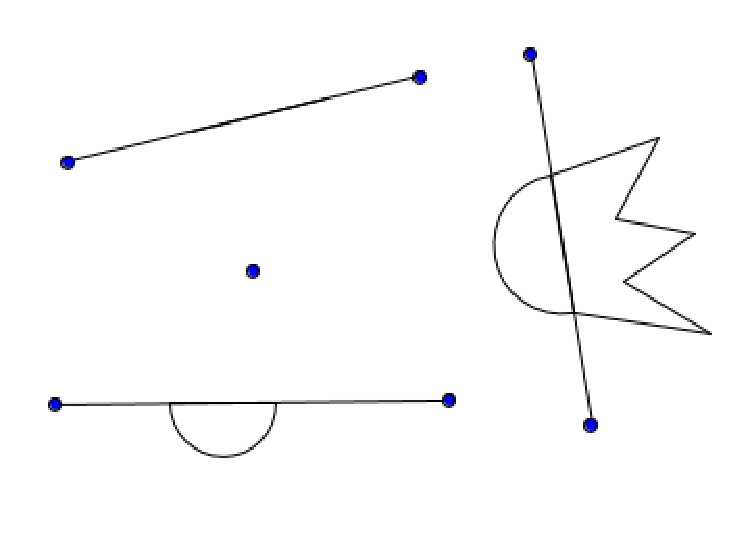
\includegraphics[scale=0.7]{Figures/TeoEsci}
\caption{El teorema de escisión nos dice que da igual qué tipo de figura adjuntemos al punto del centro en tanto que peguemos los dos extremos (resaltados en azul). Todas tendrán la misma homología relativa.}
\end{figure}

\begin{proof}
Sea $\mathcal{U}$ un recubrimiento de $X$ formado por los conjuntos $X-U$ e int$_X(A)$. Se tiene que $$\mbox{int}(X-U)=X-\overline{U} \supset X-\mbox{int}(A)$$ luego $X-U$ e int$(A)$ forman un recubrimiento de $X$. Sea $\mathcal{U}'$ el recubrimiento de $A$ formado por $A-U$ y int$_X(A)$. Por la misma razón, se tiene que int$_A(A-U)$ e int$_X(A)$ también forman un recubrimiento de $A$.
\\

En virtud del teorema 7, sabemos que los homomorfismos $$i: S_*^\mathcal{U}(X) \hookrightarrow S_*(X);\quad i': S_*^{\mathcal{U}'}(A) \hookrightarrow S_*(A)$$ forman isomorfismos entre los grupos de homología. Teniendo en cuenta que $S_*^{\mathcal{U}'}(A) \leq S_*^\mathcal{U}(X)$, la aplicación inclusión $$j: \frac{S_*^\mathcal{U}(X)}{S_*^{\mathcal{U}'}(A)} \hookrightarrow \frac{S_*(X)}{S_*(A)}=S_*(X,A)$$ forma una aplicación de cadenas que da lugar al diagrama conmutativo
\[\begin{array}{ccccccc}
H_n(S_*^{\mathcal{U}'}(A))&\longrightarrow&H_n(S_*^\mathcal{U}(X))&\longrightarrow&H_n\left(\frac{S_*^\mathcal{U}(X)}{S_*^{\mathcal{U}'}(A)}\right)&\longrightarrow&H_{n-1}(S_*^{\mathcal{U}'}(A))\\
%&&&&&&\\
i'_*\downarrow&\circlearrowleft&i_*\downarrow&\circlearrowleft&j_*\downarrow&\circlearrowleft&i'_*\downarrow\\
%&&&&&&&\\
H_n(A)&\longrightarrow&H_n(X)&\longrightarrow&H_n(X,A)&\longrightarrow&H_{n-1}(A)
\end{array}\]

Como $i_*$ e $i'_*$ son isomorfismos, el lema de los cinco nos garantiza que $j_*$ es un isomorfismo. No obstante, no relaciona los espacios que nos interesan. Ahora bien, si $A,B,C$ son grupos abelianos tales que $B+C \leq A+C$, podemos asegurar que $$\frac{A+C}{B+C} \cong \frac{A}{B} \implies S_*(X-U,A-U) \cong \frac{S_*^\mathcal{U}(X)}{S_*^{\mathcal{U}'}(A)}$$

Por tanto,
$$H_*(X,A)\cong H_*\left(\frac{S_*^\mathcal{U}(X)}{S_*^{\mathcal{U}'}(A)}\right) \cong H_*(X-U,A-U)$$
\end{proof}

\begin{ejem}
Sea $X=S^2$, $A$ el área comprendida entre los trópicos de la $S^2$ y $U$ el ecuador. Se tiene que $X-U$ son dos casquetes y $A-U$ son dos bandas. Ahora bien, observar que
$$\frac{X-U}{A-U} \cong \frac{X}{A}$$
por lo que tienen el mismo tipo de homología.

\begin{figure}[h]
\centering
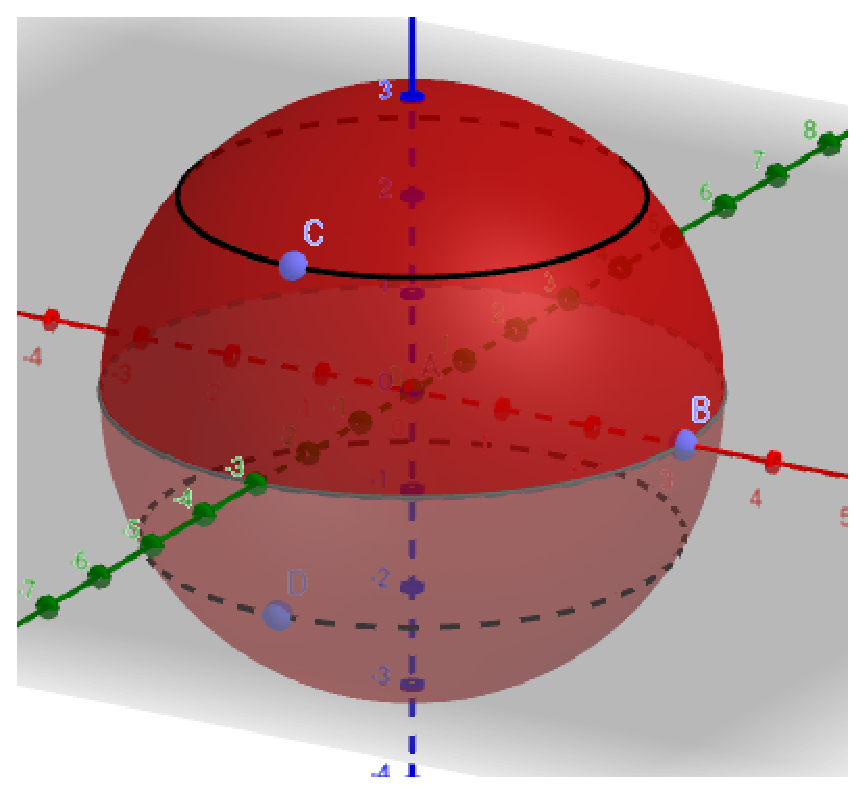
\includegraphics[scale=0.5]{Figures/EsciEsfera.eps}
\caption{Los trópicos son las circunferencias que pasan por los puntos $C$ y $D$.}
\end{figure}
\end{ejem}

\begin{ejem}
Sean $X=[0,1]^2/\sim$ el toro llano, $$A=\frac{[1/4,3/4]\times[0,1]}{\sim} \subset X$$ y $\star$ un subespacio puntual de $A$.
\\

$X-\star$ es un toro perforado. Poedmos tomar el agujero y ensancharlo hasta quedarnos con dos «hilos de alambre» cruzados (que son los generadores de $H_1$). Esos hilos forman una figura ocho.
\\

\begin{figure}[h]
\centering
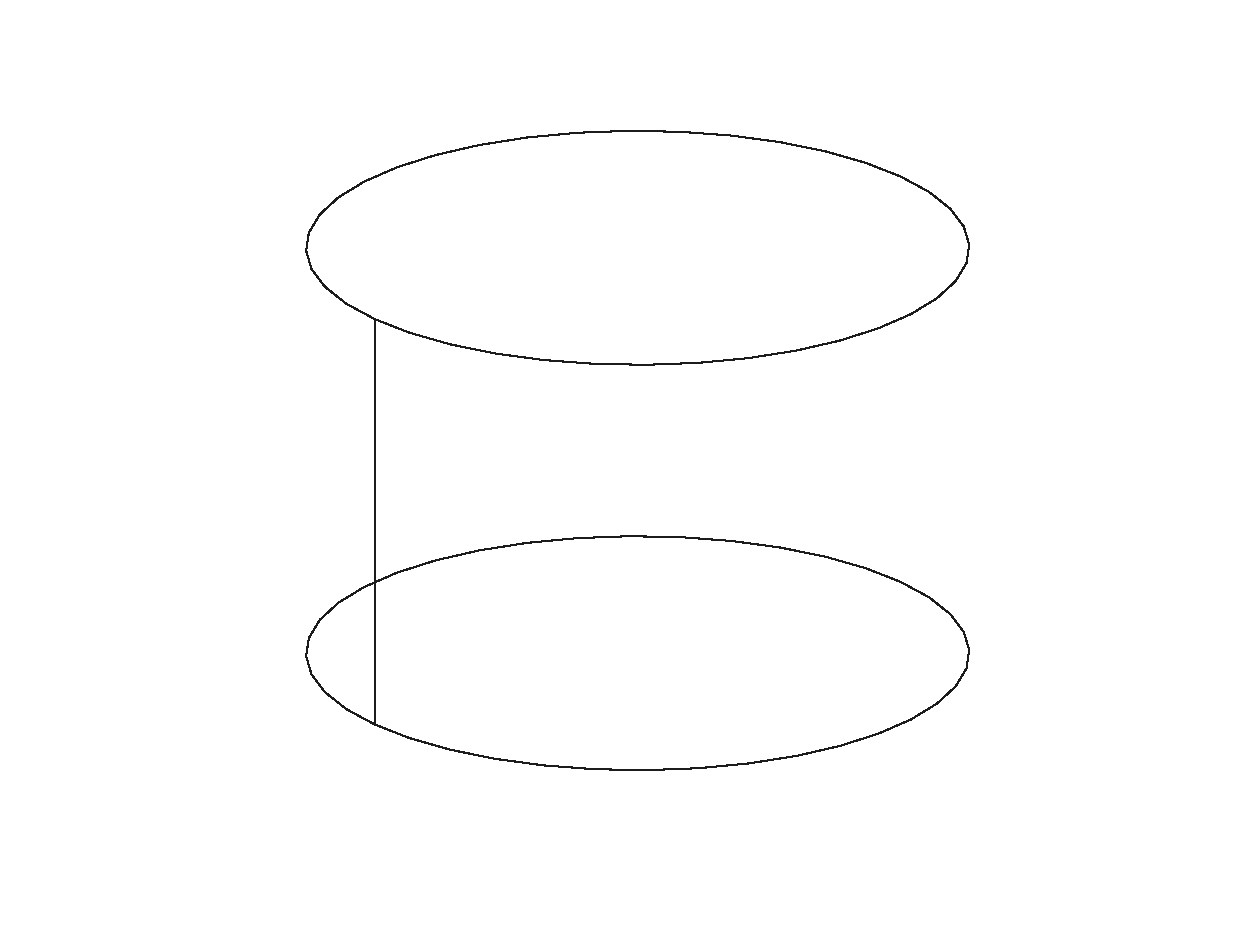
\includegraphics[scale=0.4]{Figures/1EsqCilindro.eps}
\includegraphics[scale=0.5]{Figures/FiguraOcho.eps}
\caption{Resultado de ensanchar la perforación.}
\end{figure}

Por otro lado, $A-\star$ es un cilindro perforado. Podemos tomar la perforación y ensancharla hasta quedarnos con las anillas de los bordes y un alambre que los une. Dicho alambre se puede retraer hasta que las dos anillas sean tangentes, formando una figura ocho.
\end{ejem}

\section{Grupo de homología reducida}
Sea $X \in \topo$ y $\star$ un espacio puntual. Considérese la curva $\alpha: X \longrightarrow \star$, que es claramente una aplicación constante. $\alpha$ da lugar a un homomorfismo en homologías $\alpha_*: H_*(X) \longrightarrow H_*(\star)$. \cuadro{Se define el \textbf{grupo de homología reducida} como el núcleo de dicho homomorfismo: $$\tilde{H}_*(X):=\ker \alpha_* \leq H_*(X)$$}

Observar que el espacio puntual $X=\{p\}$ es un conjunto convexo, dado que el único segmento que podemos trazar es $[p,p]=\{p\}$. Por tanto, $$\forall i > 0 \quad H_i(X)=0 \implies \tilde{H}_i(X) =0$$ Aún así, no podemos decir nada del grupo de orden 0 porque los singuletes forman espacios arcoconexos, luego $H_0(X)=\mb{Z}$.
\\

La homología reducida está creada para poder describir de forma más sencilla la homología de algunos espacios. Por ejemplo: todos los grupos de homología reducida del espacio puntual son triviales, y el único grupo de homología reducida no trivial de $S^n$ es el de orden $n$, como veremos más adelante.
\\

En general, si un espacio es arcoconexo, su grupo de homología reducida de orden cero es trivial.

\begin{prop}
Sea $X$ un espacio topológico no vacío con una cantidad finita de componentes conexas. $\tilde{H}_0(X)$ es un grupo libre que verifica $$\mbox{rk }(\tilde{H}_0(X))=\mbox{rk }(H_0(X))-1$$
\end{prop}

\begin{proof}
Sea $c$ un $0$-ciclo de $X$. Si llamamos $X_1,\dots,X_n$ a las arcocomponentes de $X$, existirán $a_1,\dots,a_n \in \mb{Z}$ tales que $$c=\sum^n_{i=1}a_ix_i \quad x_i \in X_i \quad (1 \leq i \leq n)$$ Dado que $\alpha$ es una aplicación constante, podemos llamar $\alpha_0$ al valor que toma en todos sus puntos, de forma que $$0=\alpha_*(c+B_0(X))=\sum^n_{i=1}a_i\alpha(x_i)+B_0(X)=\sum^n_{i=1}a_i\alpha_0+B_0(X)$$

De aquí se deduce que $c+B_0(X) \in \ker \alpha_*$ si y sólo si $$a_n=-\sum^{n-1}_{i=1}a_i$$ por lo que $\{x_1,\dots,x_{n-1}\}$ forma un sistema generador libre de $\tilde{H}_0(X)$. Por tanto, $$\tilde{H}_0(X) \cong \mb{Z}^{n-1} \implies \mbox{rk }(\tilde{H}_0(X))=n-1=\mbox{rk }(H_0(X))-1$$ 
\end{proof}

Ahora bien, sea $f: X \longrightarrow Y$ una aplicación continua. Al igual que $f$ induce un homomorfismo entre grupos de homología, queremos ver que $f$ induce un homomorfismo entre grupos de homología reducida. Para ello, sean $\alpha: X \longrightarrow \{p\}$, $\beta: Y \longrightarrow \{p\}$ curvas constantes y $$c=\sum^n_{i=1}a_ix_i: \quad c+B_n(X) \in \tilde{H}_n(X)$$ Se tiene que $$f_*(c+B_n(X))=\sum^n_{i=1}a_if(x_i)=\sum^m_{j=1}b_jy_j$$ Dado que las aplicaciones continuas llevan conjuntos arcoconexos en conjuntos arcoconexos, se tiene que $$\sum^n_{i=1}a_i=\sum^m_{j=1}b_j$$

Si $c+B_n(X)$ está en $\ker \alpha_*$, deberá suceder que la suma de todos los $a_i$ sea 0. Como la suma de los $a_i$ es la misma que la de los $b_j$, esto es tanto como decir que $f_*(c+B_n(X))$ está en $\ker \beta_*$. Por tanto, $f_*(\ker \alpha_*) \leq \ker \beta_*$, de forma que $f$ induce un homomorfismo $$\tilde{f}_*: \tilde{H}_*(X) \longrightarrow \tilde{H}_*(Y)$$ entre los grupos de homología reducida.

\begin{ejem} Si $X$ es un espacio contráctil, $\tilde{H}_*(X)=0$. \end{ejem}

\subsection{Una fórmula para la homología reducida}
\begin{lema}[Lema de escisión]
Sean $A,B,C$ grupos abelianos. Considérese la sucesión exacta corta $$0 \longrightarrow A \xrightarrow{f} B \xrightarrow{g} C \longrightarrow 0$$ Las siguientes afirmaciones son equivalentes:
\lista{
\item $B$ es suma directa de $A$ con $C$.
\item Existe un homomorfismo $h: B \longrightarrow A$ tal que $f\circ h=1_A$.
\item Existe un homomorfismo $k: C \longrightarrow B$ tal que $k\circ g=1_C$.}
\end{lema}

\begin{prop} Dado un $p \in X$, $$\tilde{H}_*(X)\cong H_*(X,\{p\})$$\end{prop}

\begin{proof}
Sea $i: \{p\} \hookrightarrow X$ la inclusión. La aplicación continua $$\alpha: X \longrightarrow {p}$$ verifica que $1_{\{p\}}=\alpha\circ i$, por lo que $\{p\}$ forma un retracto de $X$ e $i_*$ es un monomorfismo.
\\

Considérere la sucesión exacta de homología generada por el par de espacios $(X,\{p\})$: $$H_n(\{p\}) \xrightarrow{i_*} H_n(X) \xrightarrow{j_*} H_n(X,\{p\}) \xrightarrow{\Delta'} H_{n-1}(\{p\})$$ Como $i_*$ es un monomorfismo, $\im \Delta'=\ker i_*=0$. Por el primer teorema de isomorfia, $\im j_*=\ker \Delta'=H_n(X,p)$, por lo que $j_*$ es sobreyectiva.
\\

Dado que $i_*$ es inyectiva y $j_*$ es sobreyectiva, podemos pasar a definir una sucesión exacta corta en lugar de trabajar con una sucesión exacta larga: $$0 \longrightarrow H_n(\{p\}) \xrightarrow{i_*} H_n(X) \xrightarrow{j_*} H_n(X,\{p\}) \longrightarrow 0$$

Sabemos que $\alpha_* \circ i_*=1_{H_*(\{p\})}$, por lo que el lema de escisión nos garantiza que existe un homomorfismo $$\beta: H_n(X,\{p\}) \longrightarrow H_n(X)$$ tal que $j_*\circ \beta=1_{H_n(X,\{p\})}$. Esto es tanto como decir que $\beta$ es inyectiva.
\\

Se puede probar que $\im \beta=\ker \alpha_*=\tilde{H}_*(X)$, por lo que hemos hallado un isomorfismo entre $H_*(X,\{p\})$ y $\tilde{H}_*(X)$.
\end{proof}

Sea $X$ un espacio topológico con $n$ componentes arcoconexas. Hasta ahora, sabemos que $$\tilde{H}_0(X) \cong \mb{Z}^{n-1}$$ pero queda pregunta preguntarnos qué ocurre con los grupos de orden superior. Utilizando esta proposición que acabamos de probar, tenemos para cada $p > 0$ y el espacio puntual $\star$ que \[\tilde{H}_p(X)\cong H_p(X,\star)=\frac{Z_p(X,\star)}{B_p(X,\star)}=\frac{Z_p(X)/Z_p(\star)}{B_p(X)/B_p(\star)}\] Teniendo en cuenta que $Z_p(\star)=B_p(\star)$, estamos en condiciones de aplicar el tercer teorema de isomorfia: \[\tilde{H}_p(X)\cong \frac{Z_p(X)/Z_p(\star)}{B_p(X)/B_p(\star)}=\frac{Z_p(X)/B_p(\star)}{B_p(X)/B_p(\star)} \cong \frac{Z_p(X)}{B_p(X)}=H_p(X)\]

De esta forma, llegamos a que el grupo de homología reducida sólo \textit{reduce} el grupo de orden cero, cuya única función es contar el número de componentes conexas.

\begin{cor}
\cuadro{Sea $X$ un espacio topológico con una cantidad finita de arcocomponentes. \[\tilde{H}_*(X)\cong \frac{H_*(X)}{H_*(\star)}\]}
\end{cor}

\begin{ejem}
$$\tilde{H}_*(B_p)\cong\frac{H_*(B_p)}{H_*(\star)}\cong\begin{cases}\mb{Z}^p & \mbox{ si } n=1\\0 & \mbox{ si no}\end{cases}$$
\end{ejem}

\subsection{Homología reducida y homología relativa}
En lo sucesivo, diremos que un espacio topológico es de \textbf{tipo $C_2$} si es compacto y $T_2$ al mismo tiempo.

\begin{lema}\label{RetrCoci}
Sea $(X,A)$ un par de espacios donde $X$ es $C_2$ y $A$ es cerrado $X$. Considérese la aplicación cociente $$\pi: X \longrightarrow \frac{X}{A}$$ y sea $y=\pi(A) \in X/A$. Si $A$ es retracto por deformación fuerte de $X$, $\{y\}$ es un retracto por deformación fuerte de $\pi(X)=X/A$.
\end{lema}

\begin{nota}
Sea $X$ un espacio topológico, $\sim$ una relación de equivalencia sobre $X$ y $$\pi: X \longrightarrow X/\sim$$ una proyección.
\\

Todo punto $v \in X/\sim$ es una clase de equivalencia de $X$, y $\pi^{-1}(v)$ es el conjunto de todos sus posibles representantes.
\end{nota}

\begin{proof}
Dado que $A$ es un retracto por deformación fuerte de $X$, existe una homotopía $F: X \times I \longrightarrow X$ tal que $F_0=1_X$, $(F_t)|_A=1_A$ y $F_1(X) \subseteq A$.
\\

Si $X_A=X/A$, queremos hallar una homotopía $G: X_A\times I \longrightarrow X_A$ tal que $G_0=1_{X/A}$, $G_1(X_A,t)=\{y\}$ y $G(y,t)=y$ para todo $t \in I$. En el lema, nos proporcionan una aplicación cociente $\pi$ que envía $X$ en $X_A$ de forma continua, por lo que nuestro impulso inicial sería definir $$G=\pi \circ F \circ (\pi \times 1_I)^{-1}$$

El problema está en que $\pi^{-1}$ no está bien definida, por lo que tampoco lo va a estar $(\pi\times 1_I)^{-1}$. Lo que sí es cierto es que, de estar bien definida, la fórmula anterior sería equivalente a $$G\circ  (\pi \times 1_I)=\pi \circ F$$ Este razonamiento nos invita a definir la aplicación $$\funcio{G}{X_A\times I}{X_A}{([x]_A,t)}{(\pi \circ F)(x,t)}$$

\noindent\textbf{$G$ está bien definida y $G(y,t)=y$ para todo $t \in I$}
\\
Si $x \not\in A$, la clase de $x$ módulo $A$ es el singulete formado por el propio punto $x$, por lo que $G$ está bien definido en $X_A-\{y\}$.
\\

Por otro lado, si $x \in A$, sabemos que $$F(a,t)=a \quad \forall t \in I \implies (\pi\circ F)(a,t)=\pi(a) \in \pi(A)=\{y\}$$ De esta forma, se tiene que $G$ está bien definida y que $G_t|_A=1_A$ para todo $t \in I$.
\\

\noindent\textbf{$G$ es una deformación ($G_0=1_{X/A}$)}
\\
Sea $p \in X/A$. Si $x \in \pi^{-1}(p)$, sabemos que $F_0(x)=x$, por lo que $$G_0(p)=(\pi\circ F)(x,0)=\pi(x)=p \implies G_0=1_{X/A}$$

\noindent\textbf{$G$ es un retracto ($G_1(X/A)=\{y\}$)}\\
Sea $p \in X/A$ y $x \in \pi^{-1}(p)$. Sabemos que $F_1(x) \in A$, por lo que \[G(p,1)=(\pi \circ F)(x,1)\in \pi(A)=\{y\} \implies G(X_A,1)\subseteq\{y\}\]

\noindent\textbf{$G$ es continua}\\
Para ver que $G$ es continua, comprobaremos que la antiimagen de cualquier cerrado es cerrado.
\\

Sea $C$ un subconjunto cerrado de $X/A$. $F$ y $\pi$ son aplicaciones continuas, por lo que $D=(\pi\circ F)^{-1}(C)$ es un subconjunto cerrado de $X\times I$. Como $X\times I$ es compacto y todo subconjunto cerrado de un compacto hereda la compacidad, $D$ es compacto.
\\

$\pi$ y $1_I$ son aplicaciones continuas, por lo que $(\pi\times 1_I)(D)$ es compacto. Por cómo se define $G$, se tiene que $G^{-1}(C)=(\pi\times 1_I)(D) \subseteq X_A \times I$. Dado que $X_A\times I$ es un espacio de Hausdorff y $G^{-1}(C)$ es compacto, es cerrado.
\\

Dado que la elección de $C$ es arbitraria, se sigue que $G$ es continua.\end{proof}

\begin{lema} Sea $X$ un espacio $C_2$. Dados dos cerrados disjuntos $C,D \subset X$, existen abiertos $U,V \subset X$ tales que $U$ contiene a $C$, $V$ contiene a $D$ y $U\cap V=\emptyset$ \end{lema}

\begin{proof}
Dado un $x \in C$ y un punto $y \in D$, como $C$ y $D$ son disjuntos, $x \neq y$. Como $X$ es $T_2$, existen $U_y, V_y$ abiertos tales que $$x \in U_y \quad\land\quad y \in V_y \quad\land\quad U_y\cap V_y=\emptyset$$ Como $D$ es un subespacio cerrado de un compacto, $D$ es compacto, por lo que podemos hallar una familia finita de puntos $y_1,\dots,y_n \in D$ tales que $\{V_{y_1},\dots, V_{y_n}\}$ es un recubrimiento abierto de $D$.
\\

Para cada $i \in \{1,\dots,n\}$, podemos hallar un abierto $U_i \subseteq X$ tal que $U_i\cap V_{y_i}=\emptyset$ y $x \in U_i$. Se definen entonces $$U_x=\bigcup_{i=1}^nU_i \quad\land\quad V_x=\bigcup_{i=1}^n V_{y_i}$$ Notar que ambos conjuntos son abiertos y $U_x\cap V_x=\emptyset$.
\\

Dado que $C$ es un subespacio cerrado de un compacto, $C$ es compacto, por lo que podemos hallar una familia finita de puntos $x_1,\dots,x_n$ tales que $\{U_{x_1},\dots,U_{x_m}\}$ forma un recubrimiento abierto de $C$.
\\

Para terminar, considérense los abiertos $$U=\bigcup _{i=1}^m U_{x_i} \quad\land\quad V=\bigcup_{i=1}^m V_{x_i}$$ Se tiene que $D \subseteq V$ y $U\cap V=\emptyset$.
\end{proof}

\begin{lema}\label{LemaB} Sea $X$ un espacio $C_2$. Dado un cerrado $A$ contenido en un abierto $V$, existe un abierto $W$ tal que $$A \subseteq W \subseteq \overline{W} \subseteq V$$\end{lema}

\begin{proof}
Considérense los cerrados $A$ y $X-V$. Por el lema anterior, existen abiertos $U,W$ de $X$ tales que $A \subseteq W$, $X-V \subseteq U$ y $U\cap W=\emptyset$. $$U\cap W =\emptyset \implies W \subseteq X-U \subseteq V \implies \overline{W} \subset \overline{X-U}=X-U \subseteq V$$ Observar que $X-U$ es cerrado.\end{proof}

\begin{teo}[Teorema del retracto]
Sea $X$ un espacio $C_2$, $A$ un subespacio cerrado de $X$ y $\pi: (X,A) \longrightarrow (X/A,\pi(A))$ una aplicación cociente. Si $A$ es un retracto por deformación fuerte de algún entorno cerrado de $A$ en $X$, $$H_*(X,A) \cong H_*\left(\frac{X}{A},y\right) \cong \tilde{H}_*\left(\frac{X}{A}\right)$$
\end{teo}

\begin{proof} \textbf{Paso 1:}
\\
Considérese la sucesión exacta asociada a la tríada de espacios $(X,U,A)$: \[H_n(U,A) \xrightarrow{i_*} H_n(X,A) \xrightarrow{j_*} H_n(X,U) \xrightarrow{\Delta'} H_{n-1}(U,A)\] Dado que $A$ es un retracto por deformación fuerte de $U$, se tiene que $H_*(U,A)=0$. Por exactitud, se sigue que $0=\im i_*=\ker j_*$ y $\im j_*=\ker \Delta'=H_n(X,U)$. Por tanto, $$j_*: H_n(X,A) \xrightarrow{\quad\cong\quad} H_n(X,U)$$

\noindent\textbf{Paso 2:}
\\
Sabemos que $X$ es un espacio $C_2$ y que $A$ es cerrado. Como $U$ es entorno de $A$, $A \subseteq \mbox{int}(U)$, que es un abierto. En virtud del lema \ref{LemaB}, podemos hallar un abierto $V \subseteq X$ tal que $$A \subseteq V \subseteq \overline{V} \subseteq \mbox{int}(U) \subseteq U$$

Aplicando el teorema de escisión, se tiene que  la inclusión $$i: (X-V,U-V) \hookrightarrow (X,U)$$ induce un isomorfismo $i_*: H_*(X-V,U-V) \longrightarrow H_*(X,U)$, por lo que $$i_*^{-1}: H_*(X,U) \xrightarrow{\quad\cong\quad} H_*(X-V,U-V)$$

\noindent\textbf{Paso 3:}
\\
Considérese la aplicación $$\funcio{p}{X-V}{X_A-\pi(V)}{x}{\pi(x)}$$ Como $A \subseteq V$, se tiene que $\pi(x)$ sólo tiene un representante (al propio $x$), de forma que $p$ es un homeomorfismo. Como $\pi(U-V)=\pi(U)-\pi(V)$, se sigue que $$p_*: H_*(X-V,U-V) \xrightarrow{\quad\cong\quad} H_*(X_A-\pi(V),\pi(U)-\pi(V))$$

\noindent\textbf{Paso 4:}
\\
De la misma forma que hicimos en el paso 2, podemos aplicar el teorema de escisión al par $(X_A,\pi(U))$, con lo que se obtiene que $$i_*: H_*(X_A-\pi(V),\pi(U)-\pi(V)) \xrightarrow{\quad\cong\quad} H_*(X_A,\pi(U))$$

\noindent\textbf{Paso 5:}
\\
Considérese la sucesión exacta asociada a la tríada de espacios $(X_A,\pi(U),\pi(A))$. Procediendo de la misma forma que en el paso 1, se tiene que $$j_*: H_n(X_A,\pi(A)) \longrightarrow H_n(X_A,\pi(U))$$ es un isomorfismo, por lo que $$j_*^{-1}: H_n(X_A,\pi(U)) \xrightarrow{\quad\cong\quad} H_n(X_A,\pi(A))$$
\end{proof}

\section{Homeomorfismo relativo}
\cuadro{Un \textbf{homeomorfismo relativo} es una aplicación continua entre pares de espacios $f: (X,A) \longrightarrow (Y,B)$ tal que $$f: X-A \longrightarrow Y-B$$ es un homeomorfismo.}

\begin{ejem}Si $\m{N}=(0,0,1) \in S^2$ y $D^2$ denota a la bola unidad de $\mbR^2$, existe un homeomorfismo $$f: D^2-\partial D^2 \longrightarrow S^2-\{\m{N}\}$$ De esta forma, $f$ induce un homeomorfismo relativo entre los pares $(S^2,\{\m{N}\})$ y $(D^2,\partial D^2)$.
\\

Si $C=S^1\times I$ es un cilindro y $\m{S}$, existe un homeomorfismo $$g: S^1\times \mbox{int}(I) \longrightarrow S^2-\{\m{N},\m{S}\}$$ que identifica al cilindro sin anillas con $S^2$\end{ejem}

\begin{teo}[Teorema del homeomorfismo relativo]
Sean $X,Y$ espacios compactos de Hausdorff, $A \subseteq X$ y $B \subseteq Y$ cerrados y $f: (X,A) \longrightarrow (Y,B)$ un homeomorfismo relativo.\\

Si $A$ es retracto por deformación fuerte de algún entorno compacto de $A$ en $X$ y $B$ es retracto por deformación fuerte de algún entorno compacto de $B$ en $Y$, $f_*$ es un isomorfismo.
\end{teo}

\begin{proof}Sean $\pi: X \longrightarrow X/A$ y $\pi': Y \longrightarrow Y/B$ aplicaciones cociente. Se define la aplicación $$\funcio{f'}{X/A}{Y/B}{[x]_A}{\pi'[f(x)]}$$ Es fácil ver que $f'$ está bien definida y es continua, por lo que da lugar al siguiente diagrama conmutativo:
\[\begin{array}{ccccc}
   	&			&f        			&          	&\\
   	&X   		&\longrightarrow		&Y       	&\\
\pi	&\downarrow	&\circlearrowleft	&\downarrow	&\pi'\\
   	&X/A			&\longrightarrow		&Y/B      	&\\
    &          	&f'       			&          	&
\end{array}\]

Dado que $f$ es un homeomorfismo relativo, $f'$ es una biyección entre $X/A$ e $Y/B$. Como ambos son compactos de Hausdorff, $f'$ es un homeomorfismo, por lo que induce un isomorfismo entre $H_*(X/A)$ y $H_*(Y/B)$.
\\

Denotando $X_A=X/A$ e $Y_B=Y/B$, el diagrama conmutativo anterior induce otro diagrama conmutativo,
\[\displaystyle\begin{array}{ccc}
				&f_*        			&          		\\
H_*(X,A)   		&\longrightarrow		&H_*(Y,B)   		\\
\pi_*\downarrow	&\circlearrowleft	&\downarrow\pi'_*\\
H_*\left(X_A,\pi(A)\right)	&\longrightarrow		&H_*\left(Y_B,\pi'(B)\right)\\
          		&f'       			&          			
\end{array}\]
Sabemos por el teorema 9 que $\pi'_*$ y $\pi_*$ son isomorfismos; además, acabamos de probar que $f_*'$ es un isomorfismo. Todo ello nos lleva a que $f_*$ es un isomorfismo.
\end{proof}

\setchapterpreamble[u]{\margintoc}

\chapter{Espacios CW-complejos} \label{CW}
\section{Espacio de adjunción}
\begin{definition}
Sean $X,Y$ espacios topológicos, $A \subset X$ un subespacio cerrado y
$f\colon A \to Y$ una aplicación continua. Dados $x \in X$, $y \in Y$,
escribiremos $x \sim y$ si $x \in A$ e $y=f(x)$. Se define el
\textbf{espacio de adjunción} o \textbf{de pegamiento} como
\[X \cup_f Y:=\frac{X\sqcup Y}{\sim}\]
Decimos que $f$ es la \textbf{aplicación de adjunción} o de
\textbf{pegamiento} de $X\cup_fY$.
\end{definition}

Si $Y=\{\star\}$, $f=\text{Cte}_\star$, por lo que $x\sim z$ para todos $x,z
\in A$ y $X\cup_f Y=X/A$.

\begin{lemma}
La proyección canónica $p\colon X \sqcup Y \to X\cup_f Y$ verifica las
siguientes condiciones:
\begin{enumerate}
\item $p(Y)$ es cerrado;
\item $p|_Y$ es un homeomorfismo sobre su imagen;
\item $p(X\backslash A)$ es abierto;
\item $p|_{X\backslash A}$ es un homeomorfismo sobre su imagen.
\end{enumerate}
Como consecuencia, podemos considerar a $Y$ y $X\backslash A$ como subespacios
de $X\cup_f Y$.
\end{lemma}

\marginnote[-2.2cm]{
\begin{kaobox}[frametitle=Aplicaciones abiertas y cerradas]
Una aplicación $f\colon X \to Y$ es abierta (resp. cerrada) si la imagen de
un abierto (resp. cerrado) en $X$ es abierto (resp. cerrado) en $Y$. Si $f$ es
biyectiva, su inversa será continua si y sólo si $f$ es abierta o cerrada.

Un ejemplo de aplicación abierta (y cerrada) son las proyecciones.
\end{kaobox}
}

\begin{proof}
Como $X\sqcup Y$ es una unión disjunta de espacios topológicos, $Y$ es un
subespacio cerrado de $X\sqcup Y$. Además, $A$ es cerrado en $X$ si y sólo si
lo es en $X \sqcup Y$, por lo que $A\cup Y$ es cerrado en $X \sqcup Y$. Pero
$A\cup Y=p^{-1}[p(Y)]$, por lo que $p(Y)$ es cerrado.

Pasemos al segundo ítem: para ver que $p|_Y$ es un homeomorfismo sobre su
imagen, necesitamos ver que es cerrada e inyectiva.

Sea $y\in Y$: si $y \not\in f(A)$, se tiene de forma trivial que $p^{-1}([y])=
\{y\}$. Si $y \in f(A)$, podemos hallar un $x \in A$ tal que $f(x)=y$.

Como $x \in A \subseteq X$, podemos hallar un $y' \in X\sqcup Y$ tal que $y
\sim y'$. Si $y' \in Y$, $y=f(x)=y'$ y no hay nada que probar. Si asumimos que
$y'\neq y$, $y \in X$. Teniendo en cuenta que 
\[(p|_Y)^{-1}([y])=p^{-1}([y])\cap Y\]
se sigue que $y' \not \in (p|_Y)^{-1}([y])$, por lo que $p|_Y$ es inyectiva.

Para ver que $p|_Y$ es cerrada, sea $C$ un subespacio cerrado de $Y$. Como
$p(Y)$ es cerrado en $X \cup_f Y$, $p(C)$ es cerrado en $p(Y)$ si y sólo si lo
es en $X \cup_f Y$. Ésto es tanto como decir que $p^{-1}[p(C)]$ es cerrado en
$X \sqcup Y$.

Observamos que
\[p^{-1}[p(C)]=f^{-1}(C)\sqcup C\]
por lo que $p^{-1}[p(C)]$ es una unión de cerrados. En consecuencia, $p(C)$ es
cerrado en $p(Y)$, de donde se sigue que $p|_Y$ es una aplicación cerrada.
Ésto concluye el segundo ítem.

Como $A$ es cerrado en $X$, $X\backslash A$ es abierto en $X \sqcup Y$. Dado
que\\ $p^{-1}[p(X\backslash A)]=X\backslash A$, se sigue que
$p(X\backslash A)$ es abierto en $X\cup_f Y$.

Pasemos al último item: dado un $x \in X\backslash A$, $p^{-1}([x])=\{x\}$,
por lo que $p|_{X\backslash A}$ es inyectivo. Dado que $p$ es continua, sólo
necesitamos ver que es abierta para deducir la tesis.

Sea $U\subseteq X\backslash A$: como $p(X\backslash A)$ es abierto en
$X\cup_f Y$, $p(U)$ será abierto en $p(X\backslash A)$ si y sólo si lo es en
el espacio de adjunción, o equivalentemente, $p^{-1}[p(U)]$ es abierto en
$X\sqcup Y$.

Dado que $U\subseteq X\backslash A$, se tiene que $U=p^{-1}[p(U)]$. Si $U$
es abierto de $X\backslash A$ también lo será de $X\sqcup Y$, por lo que
$p(U)$ es abierto en el espacio de adjunción. Ésto concluye la demostración.
\end{proof}

\marginnote[-2.2cm]{
\begin{kaobox}[frametitle=Primer axioma de numerabilidad]
Un espacio topológico $X$ verifica el primer axioma de numerabilidad (1AN)
si, dado $p \in X$, existe una base de entornos numberable de $X$.

Una base de entornos de $p$ es una familia de entornos $\{V_\alpha\colon
\alpha \in A\}$ tal que, dado un entorno $U \subseteq X$ de $p$, $U$
contiene al menos a un $V_\alpha$.
\end{kaobox}
}

\begin{lemma}
\label{AdjC2} Sean $X$, $Y$ espacios de tipo $C_2$. Si $X$ e $Y$ son 1AN,
$X\cup_f Y$ es de tipo $C_2$.
\end{lemma}

\begin{proof}
El espacio $X\cup_f Y$ es compacto por ser imagen de un espacio compacto
(en este caso $X\sqcup Y$) por una aplicación continua (la proyección
canónica $p\colon X\sqcup Y \to X\cup_f Y$).

Queremos ver que $X\cup_f Y$ es $T_2$. Dado que $X\cup_f Y$ es un espacio
cociente y $X$, $Y$ son $T_2$, basta ver que el conjunto
\[\{(x,y) \in (X\cup_f Y)^2\colon y=f(x)\}=G(f)\]
es cerrado. Dado que $X$ e $Y$ son 1AN, $(X\sqcup Y)^2$ es 1AN, por lo que
$G(f)$ será cerrado si y sólo si contiene a todos sus puntos de acumulación.

\marginnote[-2.2cm]{
\begin{kaobox}[frametitle=La propiedad de Hausdorff en los cocientes]
Sea $W$ un espacio de Hausdorff y $\sim$ una relación de equivalencia sobre
los puntos de $W$. Si el conjunto
\[\{(x,y) \in W^2: x\sim y\}\]
es cerrado en $W^2$, $W/\sim$ es un espacio de Hausdorff.
\end{kaobox}
}

Sea $(z_n)$ una sucesión de $G(f)$. Por compacidad de $X \sqcup Y$, existe
una subsucesión $(z_{n_k})$ convergente a un cierto $z_0 \in X\sqcup Y$. Por
definición de $G(f)$, existe una sucesión $(x_k)$ de $A$ tal que
\[z_{n_k}=(x_k,f(x_k))\]
Se tiene entonces que $(x_k)$ converge a $x_0$, que está en $A$ por ser
cerrado de $X$. Además, como $f$ es continua, $f(x_k)$ converge a $f(x_0)$.

De esta forma, $(z_{n_k})$ converge a $(x_0,f(x_0)) \in G(f)$. Dado que
$X\sqcup Y$ es $T_2$, $z_0=(x_0,f(x_0))$, por lo que $z_0 \in G(f)$. De aquí
se sigue que $G(f)$ es cerrado. Por tanto, $X\cup_f Y$ es $T_2$.
\end{proof}

\begin{lemma}\lablemma{RepAdj}
Sean $X$, $Y$, $W$ espacios $C_2$, $A \subset X$ un subconjunto cerrado y
$g\colon X\sqcup Y \to W$ una aplicación continua y sobreyectiva. Supongamos
que, para todo punto $w \in W$, se cumple que
\[g^{-1}(w)=\left\{
\begin{array}{c}
\text{un único punto de $X\backslash A$}\\
\lor\\
\text{$\{y\}\cup f^{-1}(y)$ para algún $y \in Y$}
\end{array}
\right.\]
Entonces, $g$ induce un homeomorfismo entre $W$ y $X \cup_f Y$.
\end{lemma}

\begin{proof}
Sea $\p\colon X\sqcup Y \to X \cup_f Y$ la proyección canónica. Se define la
aplicación
\begin{diag}
\overline g\colon X\cup_f Y \arrow[r]& W\\[-8mm]
\left[x\right] \arrow[maps to, r] & g(x)
\end{diag}

\marginnote[-2.2cm]{
\begin{kaobox}[frametitle=Continuidad de la inversa]
Si $f\colon X \longrightarrow Y$ es una biyección continua, donde $X$ es
compacto e $Y$ es de Hausdorff, $f$ es un homeomorfismo.
\end{kaobox}
}

Supongamos que $\overline g$ está bien definida y es una biyección continua:
por el \reflemma{AdjC2}, tenemos que $X\cup_f Y$ es de tipo $C_2$. Como $W$ es
$T_2$, se sigue que $\overline g$ tiene inversa continua, por lo que es un
homeomorfismo y el lema queda probado.

Empecemos por ver que $\overline{g}$ está bien definida: sean $x_1, x_2 \in
A$ elementos asociados y diferentes. Existirá un $y \in f(A)$ tal que $f(x_1)=
y=f(x_2)$. Si $w=g(x_1)$, se tiene por hipótesis que
\[g^{-1}(w)=\{y\}\cup f^{-1}(y) \implies g(x_1)=w=g(x_2)\]
Si $x \in X\backslash A$, $x$ sólo está asociado consigo mismo, de forma que
$\overline{g}$ está trivialmente bien definida. Dado que todas las
antiimágenes por $g$ de un cierto $w \in W$ están asociadas, $\overline{g}$ es
también inyectiva.

Veamos que $\overline{g}$ es continua: si $C \subseteq W$ es cerrado,
$g^{-1}(C)$ es cerrado en $X\sqcup Y$, por lo que $\pi^{-1}[g^{-1}(C)]$ es
cerrado en $X\cup_f Y$. Notar que
\[\pi^{-1}[g^{-1}(C)]=\overline{g}^{-1}(C)\]
por lo que se sigue la continuidad de $\overline{g}$.
\end{proof}

Sea $g\colon X \to W$ una aplicación continua y sobreyectiva entre espacios de
tipo $C_2$. Supongamos que existe un $w_0 \in W$ de forma que $A=g^{-1}(w_0)$
es un cerrado en $X$ y $g^{-1}(w)$ es un único punto de $X\backslash A$ para
todo $w\neq w_0$.

Si $\{\star\}$ es el espacio puntual, la aplicación constante
$f\colon A \to \{\star\}$ es continua, y se verifica que $X \cup_f \{\star\}$
es homeomorfo a $X/A$. Por el \reflemma{RepAdj}, se tiene que
\[W \cong X \cup_f \{\star\}\cong X/A\]

%Un espacio topológico Hausdorff y 2AN $X$ es una $n$-variedad si, dado $p \in
%$X$, existe un entorno abierto $U \subseteq X$ de $p$ homeomorfo a una bola
%abierta de $\mb{R}^n$. Éstos homeomorfismos se denominan cartas o
%parametrizaciones locales de $X$.

\begin{example} \label{Sn_CW}
Sea $h\colon D^n\backslash S^{n-1} \to \mb{R}^n$ un homeomorfismo, $\mc{N}=
(0,0,\dots,0,1)$ y $S^n_+=S^n\backslash\mc{N}$. La \textbf{proyección
estereográfica}, dada por
\begin{diag}
\Phi\colon S^n_+ \arrow[r] & \mb{R}^n\\[-8mm]
(x_1,\dots,x_{n+1}) \arrow[maps to, r] &
	\displaystyle\left(\frac{x_1}{1-x_{n+1}},\dots,\frac{x_n}{1-x_{n+1}}\right)
\end{diag}
es un homeomorfismo. Una posible parametrización de $h$ es
\[h(z)=\frac{z}{1-\|z\|}\]
Se define la aplicación $g\colon D^n \to S^n$ dada por
\[g(x)=\begin{cases}
\mc{N} &\text{ si $x \in S^{n-1}$}\\
(\Phi^{-1}\circ h)(x) &\text{ si $x \in D^n\backslash S^{n-1}$}
\end{cases}\]
Se tiene entonces que $g$ es continua y sobreyectiva por construcción.

Como $\mc{N} \in S^{n-1}$, $g^{-1}(\mc{N})=\{\mc{N}\}$ es un cerrado en $D^n$.
Dado que $\Phi$ y $h$ son aplicaciones biyectivas, $g^{-1}(z)$ es un único
punto para todo $z\neq \mc{N}$. Aplicando el lema \reflemma{RepAdj}, se tiene
entonces que
\[S^n\cong \frac{D^n}{S^{n-1}}\]
que es la adjunción de $D^n$ a un espacio puntual.
\end{example}

\begin{marginfigure}
\resizebox{\textwidth}{!}{
\begin{tikzpicture}
\draw[fill=blue] (0,0) circle (1pt);

\draw[dashed, -to] (.8,.8) -- (.2,.2);
\draw[dashed, -to] (.8,-.8) -- (.2,-.2);

\draw[fill=blue] (1,1) circle (1pt) -- (1,-1) circle (1pt);

\draw[|-stealth] (1.5,0) -- (2,0);

\draw (3.5,0) node {$S^1$} circle (1cm);
\draw[fill=blue] (2.5,0) circle (1pt);
\end{tikzpicture}
}
\caption{\labfig{CWS1} Conjunto $S^1$ construido como espacio de adjunción.}
\end{marginfigure}
\begin{marginfigure}
\resizebox{\textwidth}{!}{
\begin{tikzpicture}
\draw (3.5,0) circle (1cm);
\draw[fill=blue] (2.5,0) circle (1pt);

\draw (3.5,-1) .. controls (2,-1) and (1.5,0) .. (0,0);
\draw (3.5,1) .. controls (2,2) and (1.5,0) .. (0,0);
\end{tikzpicture}
}
\caption[Espacio $S^1$ con dos segmentos adicionales, creando una figura
ocho.]{Podemos adjuntar nuevas células a las células preexistentes para
recrear espacios más complejos.}
\end{marginfigure}


\subsection{Células y adjunción}
Supongamos que $X=D^n$ para algún $n > 0$ y $A=S^{n-1}=\p D^n$. Decimos que el
espacio
\[Y_f:=D^n\cup_f Y\]
es la \textbf{adjunción de una $n$-célula} al espacio $Y$.

\begin{example}\labexample{Sn_CW}
En la figura \reffig{CWS1}, vemos cómo $S^1\cong \{\star\}_f$, siendo
$f\colon \p D^1=\{0,1\}\to \{\star\}$ la aplicación constante. En general,
$S^n$ se puede obtener como $\{\star\}_{f_n}$, siendo $f_n\colon \p D^n \to
\{\star\}$.
\end{example}

\begin{lemma}\lablemma{EntornoCompacto}
Sea $f: S^{n-1} \to Y$ una aplicación continua. Si $Y$ es un espacio $C_2$,
existe un entorno compacto $U_f$ de $Y$ en $Y_f$ tal que $Y$ es un retracto
por deformación fuerte de $U_f$.
\end{lemma}

\begin{proof}
Sea $U=\{x \in D^n: \|x\| \geq 1/2\}$. El cerrado $U$ es un entorno compacto
de $S^{n-1}$ en $D^n$. Definimos la homotopía $F\colon (U \sqcup Y)\times I
\to U\sqcup Y$ como
\[F(x,t)=
\begin{cases}
x &\text{ si }x \in Y \\
\displaystyle
(1-t)x+t\frac{x}{\|x\|} &\text{ si }x \in U
\end{cases}\]

Tenemos que $F$ es una aplicación continua que verifica las siguientes
propiedades:
\begin{enumerate}
\item $F(x,0)=x$ para todo $x \in U\sqcup Y$.
\item $F(x,1) \in S^{n-1}\sqcup Y$ para todo $x \in U \sqcup Y$.
\item $F(x,t)=x$ para todo $x \in S^{n-1}\sqcup Y$ y todo $t \in I$.
\end{enumerate}
Se sigue que $S^{n-1}\sqcup Y$ es un retracto por deformación fuerte de
$U\sqcup Y$.

Si $p\colon D^n \sqcup Y \to Y_f$ denota a la proyección canónica, se define
$U_f$ como la imagen de $U$ mediante $p$. Queremos ver que $Y$ es un retracto
por deformación fuerte de $U_f$ en $Y_f$. Para ello, considérese la
homotopía
\begin{diag}
G\colon U_f\times I \arrow[r] & U_f\\[-8mm]
(\left[x\right],t)\arrow[maps to,r] & F(x,t)
\end{diag}

Es fácil ver que $G$ está bien definida. Para ver que es continua, considérese
el diagrama conmutativo
\begin{diag}
(U\sqcup Y)\times I \arrow{r}{F} \arrow{d}{p\times \id_I}&
	U\sqcup Y \arrow{d}{p}\\
U_f\times I \arrow{r}{G} & U_f
\end{diag}

Dado que $F$ y $p$ son continuas, $G\times (p\times \id_I)=p\circ F$ es
continua, por lo que $G$ es continua. De aquí se sigue que $Y$ es un retracto
por deformación fuerte de $U_f$.
\end{proof}

\begin{proposition}
Dada una aplicación continua $f\colon S^{n-1} \to Y$,
\[H_p(Y_f,Y)\cong
\begin{cases}
\mb{Z} & \text{ si $p=n$}\\
0 & \text{ si no}
\end{cases}\]
\end{proposition}

\begin{proof}
Consideremos la composición
\[h\colon D^n \hookrightarrow D^n\sqcup Y \xrightarrow{p} Y_f\] 
El espacio $D^n\backslash S^{n-1}$ es homeomorfo a $Y_f\backslash Y$, puesto
que $Y_f=Y\cup_f D^n$, de forma que $h$ induce un homeomorfismo relativo entre
los pares $(D^n,S^{n-1})$ e $(Y_f,Y)$.

La esfera $S^{n-1}$ es un retracto por deformación fuerte del entorno compacto
$U=\{x \in D^n: \|x\| \geq 1/2\}$, y sabemos por el
\reflemma{EntornoCompacto} que $Y$ es un retracto por deformación fuerte de
algún entorno $U_f$ compacto de $Y$ en $Y_f$. Por el teorema del homeomorfismo
relativo (\refthm{HomeoRelativo}), se tiene que
\[h_*\colon H_*(D^n,S^{n-1}) \longrightarrow H_*(Y_f,Y)\]
es un isomorfismo.

Se tiene entonces que
\[H_*(Y_f,Y) \cong H_*(D^n,S^{n-1}) \cong \tilde{H}_*(S^n)\cong
\begin{cases}
\mb{Z} & \text{ si }p=n \\
0 & \text{ si no}
\end{cases}\]
\end{proof}

\begin{proposition} \labprop{HomoCW}
Sea $Y$ un espacio topológico y $f\colon S^{n-1} \to Y$ una aplicación
continua. Si $f_*\colon \tilde{H}_{n-1}(S^{n-1}) \to H_{n-1}(Y)$,
\begin{enumerate}
\item $H_p(Y_f)\cong H_p(Y)$ para todo $p$ distinto a $n$ y $n-1$;
\item $H_{n-1}(Y_f)\cong H_{n-1}(Y)/\im f_*$;
\item la sucesión
\begin{diag}
0 \arrow[r]& H_n(Y) \arrow[r]& H_n(Y_f) \arrow[r]&
\ker f_* \arrow[r]& 0
\end{diag}
es exacta.
\end{enumerate}
\end{proposition}

\begin{proof}
Consideremos la sucesión exacta larga asociada al par de espacios $(Y_f,Y)$:
\[\dots \longrightarrow H_{p+1}(Y_f,Y) \longrightarrow H_p(Y)
\xrightarrow{\beta} H_p(Y_f) \longrightarrow H_p(Y_f,Y) \longrightarrow \dots\]
Como vimos en el \refexample{Sn_CW},
\[H_p(Y_f,Y)\cong \tilde{H}_p(S^n) \cong \tilde{H}_{p-1}(S^{n-1})\]

Para $p\neq n,n-1$, $\tilde{H}_p(S^n)=0$, por lo que $\ker
\beta=0$ y $\im \beta=H_p(Y_f)$. Se sigue entonces la primera afirmación:
\[H_p(Y_f) \cong H_p(Y)\]

Para $p=n$ y $p=n-1$, se tiene la sucesión exacta
\begin{align*}
0=\tilde{H}_n(S^{n-1}) &\longrightarrow H_n(Y) \longrightarrow H_n(Y_f)
\xrightarrow{\beta} \tilde{H}_{n-1}(S^{n-1}) \xrightarrow{f_*} \\
&\xrightarrow{f_*} H_{n-1}(Y) \xrightarrow{\alpha} H_{n-1}(Y_f)
\longrightarrow \tilde{H}_{n-2}(S^{n-1})=0
\end{align*}
donde $\im \beta=\ker f_*$, $\im f_*=\ker \alpha$ y $\im \alpha=H_{n-1}(Y_f)$
por exactitud. Aplicando el primer teorema de isomorfia, se tiene la segunda
afirmación:
\[H_{n-1}(Y_f)=\im \alpha \cong \frac{H_{n-1}(Y)}{\ker \alpha}=
\frac{H_{n-1}(Y)}{\im f_*}\]

Ahora bien: como $\im \beta=\ker f_*$, la sucesión
\[0 \longrightarrow H_n(Y) \longrightarrow H_n(Y_f) \xrightarrow{\beta}
\ker f_* \longrightarrow 0\] es exacta, que es la tercera afirmación.
\end{proof}

\section{Espacios CW-complejos}
Sean $D_1^n,\dots, D_p^n$ una familia de $n$-células disjuntas con respectivas
fronteras $S^{n-1}_1,\dots,S^{n-1}_p$. Dado un $1 \leq i \leq p$, considérese
la aplicación continua
\[f_i\colon S^{n-1}_i \longrightarrow Y\]
siendo $Y$ un espacio topológico arbitrario. Si $\mc{D}^n=D^n_1\sqcup\dots
\sqcup D^n_p$ y $\mc{S}^{n-1}=\p \mc{D}^n=S^{n-1}_1\sqcup \dots S^{n-1}_p$,
definimos sobre $\mc{D}^n\sqcup Y$ la siguiente relación de equivalencia:
\[\forall x \in S^{n-1}_i \quad x \sim f_i(x); \quad i=1,\dots,p\]
Definimos entonces el espacio
\[Y_{f_1,\dots,f_p}=\frac{\mc{D}^n\sqcup Y}{\sim}\]

\begin{proposition}
Sea $(X,Y)$ un par de espacios $C_2$. Si existe un homeomorfismo relativo
\[F\colon (\mc{D}^n,\mc{S}^{n-1})\longrightarrow(X,Y)\]
que sea una prolongación continua de $f_1,\dots,f_p$, entonces $X$ es
homeomorfo a $Y_{f_1,\dots,f_p}$.
\end{proposition}

\begin{marginfigure}
\centering
\begin{subfigure}[b]{\textwidth}
\resizebox{\textwidth}{!}{
\begin{tikzpicture}

\draw[fill=green] (0,2) circle (1pt) -- (1.4,2) circle (1pt);
\draw[dashed, -stealth] (.1,2-1/7) -- (.6,2-6/7);

\draw[fill=green] (.7,1) circle (1pt);

\draw[dashed, -stealth] (.1,1/7) -- (.6,6/7);
\draw[dashed, -stealth] (1.3,2-13/7) -- (.8,2-8/7);

\draw[fill=green] (0,0) circle (1pt) -- (1.4,0) circle (1pt);

\draw[|-stealth] (1.5,1) -- (3,1);

\draw (4,1) circle (.7cm);
\draw[fill=green] (4,1.7) circle (1pt) -- (4,2.7) circle (1pt);

\end{tikzpicture}
}
\caption{Usando $1$-células, podemos construir un complejo de dimensión
$1$...}
\end{subfigure}
\begin{subfigure}[b]{\textwidth}
\resizebox{\textwidth}{!}{
\begin{tikzpicture}
\draw (0,0) circle (.7cm);
\draw[fill=green] (0,.7) circle (1pt) -- (0,1.7) circle (1pt);

\draw[|-stealth] (1.2,0) -- (2,0);

\draw[pattern=north west lines, pattern color=blue]
	(3,0) circle (.7cm) node {\contour{white}{$D^2$}};
\draw[fill=green] (3,.7) circle (1pt) -- (3,1.7) circle (1pt);


\end{tikzpicture}
}
\caption{...y después añadir células de orden superior, creando figuras más
complejas como una piruleta.}
\end{subfigure}
\end{marginfigure}

\begin{definition}
\begin{enumerate}
\item Un \textbf{CW-complejo finito de dimensión 0} es una colección finita de
puntos $\{p_1,\dots,p_n\} \subset \mb{R}^t$.
\item Sea $Y$ un CW-complejo finito de dimensión $k \geq 0$. Un espacio
topológico $C_2$ $X$ es un \textbf{CW-complejo finito de dimensión $n$} si
existen $f_i\colon S^{n-1} \longrightarrow Y$, $i=1,\dots,s$, tales que $X$ es
homeomorfo a $Y_{f_1,\dots,f_s}$.
\end{enumerate}
\end{definition}

Hemos definido los CW-complejos de dimensión $n$ como un proceso iterativo que
da lugar a una serie de CW-complejos intermedios
\[X^0 \subseteq X^1 \subseteq \dots \subseteq X^n\]
Cada uno de los $X^k$ se denomina \textbf{$k$-esqueleto} del CW-complejo. Notar
que $X^n$ es el CW-complejo completo.

\begin{example}\labexample{S2CW}
El \refexample{Sn_CW} describe una construcción de $S^2$ como CW-complejo de
forma que el 1-esqueleto y el 0-esqueleto son el mismo conjunto, porque no
adjuntamos ninguna 1-célula a $X^0$. Pero un CW-complejo puede admitir muchas
estructuras diferentes. 

Consideremos la siguiente estructura: sean
\[X^0=\{(1,0,0), (0,1,0),(-1,0,0)\}\]
tres puntos del ecuador. Adjuntamos a $X^0$ tres 1-células, $D^1_1$, $D^1_2$
y $D^1_3$, de forma que $S^1\cong X^1$.

Finalmente, adjuntamos dos 2-células $D^2_1$ y $D^2_2$ a $X^1$. Esto sería
$X^2$, que es homeomorfo a todo $S^2$.

En general, podemos generar una descomposición de $S^n$ de forma que cada
$k$-esqueleto sea $S^k$ ($k=0,1,2,\dots,n$); no obstante, en ese caso
tendríamos que el 0-esqueleto son dos puntos, dado que
\[S^0=\{x \in D^1: \|x\|=1\}=\{x \in [-1,1]: |x|=1\}=\{\pm 1\}\]
\end{example}

\begin{marginfigure}
\includegraphics{Figures/S2CW.pdf}
\caption{Espacio $S^2$ construido utilizando el \refexample{S2CW}.}
\end{marginfigure}

De esta forma, tenemos que un espacio topológico no induce una descomposición
como CW-complejo de forma única. Si comparamos este proceso con el que
seguimos en el \refexample{Sn_CW}, tenemos que no tienen el mismo número de
células y sus $1$-esqueletos no son homeomorfos, de forma que no son
\textit{estructuras equivalentes}.

\begin{theorem}[Caracterización de CW-complejos finitos]\labthm{TCCWF}
Un espacio topológico compacto $X$ es un CW-complejo finito de dimensión $n$
si y sólo si podemos hallar una sucesión de subespacios
\[X^0 \subseteq X^1 \subseteq \dots \subseteq X^n=X\]
y una partición de subconjuntos
\[\{D_i^k:\; k=0,1,\dots,n; \;i=1,2,\dots,r_k\}\]
(llamada \textbf{descomposición celular}) tales que
\begin{enumerate}
\item existe un homeomorfismo relativo
\[h\colon (D^k,S^{k-1}) \to
(\overline{D^k_i},\overline{D^k_i}\backslash D^k_i)\]
para cada $i$ y $k$;
\item dado un $1 \leq k \leq n$, $\overline{D^k_i}\backslash D^k_i
\subseteq X^{k-1}$.
\end{enumerate}
\end{theorem}

Hagamos un par de incisos en este teorema.

\begin{itemize}
\item Observar que $\overline{D^k_i}\backslash(\overline{D^k_i}\backslash
D^k_i)=D^k_i$. Aplicando el teorema anterior, se sigue que $D^k_i$ es
homeomorfo a una bola abierta de $\mb{R}^k$. Esto implica que las $n$-células
son conexas, compactas y abiertas para todo $n > 0$.
\item La condición de compacidad viene dada porque la adjunción de espacios
compactos es compacto, pero ninguna de las otras condiciones garantizan que
$X$ sea compacto.
\end{itemize}

\begin{example}
\begin{enumerate}
\item Este teorema proporciona otra forma de ver que $S^n$ admite una
estructura de CW-complejo: para $n=1$, sea $f\colon [0,2\pi] \to \mb{R}^2$ la
aplicación $f(t)=(\cos t,\sin t)$. Tenemos que $X=S^1$ admite una estructura
de CW-complejo tomando
\begin{align*}
X^0&=\{(1,0)\}; 	& X^1&=S^1;\\
D^0&=\{(1,0)\}; 	& D^1&=f(]0,1[]);
\end{align*}
Para $n=2$, sea $g\colon [0,1]\times [0,1] \to \mb{R}^3$ la aplicación
\[g(u,v)=(\cos(2\pi u)\cos(2\pi v),\cos(2\pi u)\sin(2\pi v),\sin(2\pi u))\]
Entonces, $Y=S^2$ admite una estructura de CW-complejo tomando
\begin{align*}
Y^0		&=\{(1,0,0)\}; 	& D^0&=\{(1,0,0)\};\\
Y^1 	&=S^1 			&
D^2_1	&=g([0,1]\times(]0,3/4[\cup]3/4,1[));\\
D^1 	&=g([0,1]\times\{0\});	&
D^2_2	&=g([0,1]\times(]1/4,3/4[]));
\end{align*}
\item El segmento $I$ admite una estructura de CW-complejo dada por la
descomposición celular $\{\{0\},\{1\},]0,1[\}$. En general, toda línea
poligonal formada por una cantidad finita de segmentos admite una estructura
trivial de CW-complejo.
\end{enumerate}
\end{example}

\begin{example}
\begin{enumerate}
\item El conjunto $A=\{1/n: n \in \mb{N}\}\cup \{0\}$ con la topología
inducida por la métrica usual de $\mb{R}$ no es un CW-complejo finito, porque
no es compacto.

\item El \textbf{pendiente hawaiiano} es un ejemplo de espacio topológico
compacto que no tiene estructura de CW-complejo. Si $C(\alpha,\beta)$ denota
la circunferencia de centro $\alpha \in \mb{R}^2$ y radio $\beta > 0$, se
define el pendiente hawaiiano como el espacio topológico
\begin{align*}
H=\bigcup_{n=1}^\infty C(\alpha_n,\beta_n) &&
\left(\alpha_n=\left(\frac{1}{n},0\right), \quad 
\beta_n=\frac{1}{n}\right)
\end{align*}
Intuitivamente, esto se debe a que tiene una cantidad infinita de anillos, y
cada uno tendría que ser una 1-célula independiente.
\end{enumerate}
\end{example}

\begin{marginfigure}
\resizebox{\textwidth}{!}{
\begin{tikzpicture}[scale=0.1]
\foreach \n in {4,...,20}
	\draw (\n,0) circle (\n cm);
\end{tikzpicture}
}
\caption{Primeras $16$ iteraciones del pendiente hawaiiano.}
\end{marginfigure}

\begin{proposition}\labprop{CWProd}
El producto de CW-complejos finitos es un CW-complejo finito.
\end{proposition}

\begin{proof}
Sean $\mc{C}=\{D_i^k:\; k=0,1,\dots,n; \;i=1,2,\dots,r_k\}$ y $\mc{D}=
\{\Delta_\ell^j:\; j=0,1,\dots,m; \;\ell=1,2,\dots,r_j\}$ respectivas
descomposiciones celulares de $X$ e $Y$. Queremos ver que el conjunto
\[\mc{E}=\{U\times V: U\in \mc{C}, V\in \mc{D}\}\]
forma una descomposición celular de $X\times Y$.

Claramente, los elementos de $\mc{E}$ son disjuntos dos a dos por
construcción. Veamos que forman un recubrimiento de $X\times Y$: 
\[X\times Y=
	\left(\bigcup_{U \in \mc{C}} U\right)\times
	\left(\bigcup_{V \in \mc{D}} V\right)=
	\bigcup_{\substack{U \in \mc{C}\\V \in \mc{D}}} U\times V\]

Para demostrar este resultado, aplicaremos el \refthm{TCCWF}: dados
$i,j,k,\ell$,
\begin{align*}
U&=(\overline{D^k_i\times \Delta^\ell_j})\backslash
	(D^k_i\times \hat D^\ell_j)=
	(\overline{D^k_i}\times \overline{\Delta^\ell_j})\backslash
	(D^k_i\times \hat D^\ell_j)=\\
	&=[(\overline{D^k_i}\backslash D^k_i)\times \overline{\Delta^\ell_j}]\cup
	[\overline{D^k_i}\times (\overline{\Delta^\ell_j}\backslash \Delta^\ell_j)]
\end{align*}
Sabemos por hipótesis que $(\overline{D^k_i}\backslash D^k_i) \subseteq
X^{k-1}$ y $\overline{\Delta^\ell_j}\backslash \Delta^\ell_j \subseteq
Y^{\ell-1}$, por lo que $U \subseteq (X\times Y)^{k+\ell-1}$. Esto prueba la
primera condición.

Pasemos a la segunda: sean $U \in \mc{C}$ y $V \in \mc{D}$. Si
\begin{align*}
f\colon (D^k,S^{k-1}) \to (\overline{U},\overline{U}\backslash U); &&
g\colon (D^\ell,S^{\ell-1}) \to (\overline{V},\overline{V}\backslash V)
\end{align*}
son homeomorfismos relativos, se tiene que
\[f\times g\colon (D^{k+\ell},S^{k+\ell-1}) \to
(\overline{V\times V},(\overline{U\times V})\backslash (U\times V))\]
es un homeomorfismo relativo.
\end{proof}

\begin{example}\labexample{CWlindro}
\begin{enumerate}
\item El cilindro con bordes se define como $C=S^1\times [0,1]$. Podemos
asignar una estructura de CW-complejo a $C$ usando una estructura prefijada
de $S^1$ y otra de $[0,1]$:

\begin{align*}
[0,1]
\begin{cases}
\text{0-células:}	&p=\{0\}\\
					&q=\{1\}\\
\text{1-células:}	&\alpha=]0,1[
\end{cases}
&&
S^1
\begin{cases}
\text{0-células:}	&r=\{(1,0)\}\\
\text{1-células:}	&\beta=S^1-r
\end{cases}
\end{align*}

Estas estructuras inducen la siguiente descomposición celular sobre el cilindro:
\[C \begin{cases}
\text{0-células:}	&p\times r, q\times r\\
\text{1-células:}	&\alpha \times r, p\times \beta, q\times \beta\\
\text{2-células:}	&\alpha \times \beta
\end{cases}\]

\item El toro se puede expresar como $S^1\times S^1$, por lo que admite una
estructura de CW-complejo finito.

Consideremos la siguiente descomposición celular de $S^1$:
\begin{align*}
S^1
\begin{cases}
\text{0-células:}	&p=\{(1,0)\}\\
\text{1-células:}	&\alpha=S^1-p
\end{cases}
&&
S^1
\begin{cases}
\text{0-células:}	&r=\{(1,0)\}\\
\text{1-células:}	&\beta=S^1-r
\end{cases}
\end{align*}

Estas estructuras inducen la siguiente descomposición celular sobre el toro:
\[S^1\times S^1
\begin{cases}
\text{0-células:}&p\times r\\
\text{1-células:}&\alpha \times r,p\times \beta\\
\text{2-células:}&\alpha \times \beta
\end{cases}\]
\end{enumerate}
\end{example}

\begin{marginfigure}
\resizebox{\textwidth}{!}{
\begin{tikzpicture}
\draw (2,0) circle (.9cm);
\draw (1.1,0) -- (-.1,0);
\draw (-1,0) circle (.9cm);
\end{tikzpicture}
}
\caption[1-esqueleto del cilindro.]{1-esqueleto del cilindro. Observar que se
puede retraer en una figura ocho.}
\end{marginfigure}

\begin{marginfigure}
\includegraphics{Figures/ToroGeneradoresOrden1.pdf}
\caption{1-esqueleto del toro.}
\end{marginfigure}

\subsection{Subcomplejos}
Sea $X$ un CW-complejo finito y $\mc{C}$ una descomposición celular de $X$.
Decimos que un subespacio $A \subseteq X$ es un \textbf{subcomplejo} de $X$ si,
dado $D \in \mc{C}$, $D\cap A \neq \emptyset$ implica que $\overline{D}
\subseteq A$. Esta condición se puede expresar como que $A$ absorbe a todas
las células con las que entra en contacto.

Todo subcomplejo de un cierto complejo $X$ conforma un subespacio cerrado.
Además, aplicando el \refthm{TCCWF}, todo subcomplejo es un complejo en sí
mismo. En particular, todos los $k$-esqueletos de $X$ son subcomplejos.

\begin{proposition}
Si $A$ es un subcomplejo de un CW-complejo finito $X$, $A$ es un retracto por
deformación fuerte de algún entorno compacto de $A$ en $X$.
\end{proposition}

\begin{proof}
Sea $N$ el número de células que componen el espacio $X\backslash A$. Si
$N=0$, $X=A$, por lo que $A$ es un retracto por deformación fuerte de $X$ de
forma trivial y se sigue la tesis por compacidad de $X$.

Si $N=1$, existe una aplicación $f\colon S^{n-1} \to A$ continua tal que
$X=A\cup_f D^n$. En tal caso, podemos limitarnos a aplicar el
\reflemma{EntornoCompacto}.

Supongamos que el resultado es cierto para cualquier par de CW-complejos
finitos $(Y,B)$ tales que $Y\backslash B$ posee a lo sumo $N-1$ células, y sea
$(X,A)$ un par de CW-complejos tales que $X\backslash A$ tiene exactamente $N$
células. Si $D^m_i$ es una célula de $X\backslash A$ de dimensión máxima, se
define el subespacio $Y=X\backslash D^m_j$.

Queremos ver que $Y$ es un subcomplejo de $X$. Como $D^m_i$ es una célula de
dimensión máxima, todas las células de $X\backslash A$ tienen dimensión $m$ o
menos; de esta forma, toda célula de $X$ con dimensión mayor que $m$ forma
parte del subcomplejo $A$. En consecuencia, si $D^k_j$ es una célula de $Y$,
se tiene que $D^k_j \subset A$ ó $k \leq m$.

Si $D^k_j \subset A$, $\overline{D^k_j} \subseteq A$ por ser $A$ un
subcomplejo de $X$, de forma que
\[D^m_i \cap \p D^k_j \subseteq D^m_i \cap A=\emptyset\]
En cambio, si $k \leq m$, se tiene por \refthm{TCCWF} que
\[\p D^k_j=\overline{D^k_j}\backslash D^k_j\subseteq X^{k-1}\]
Dado que $k-1 < m$, se cumple una vez más que $D^m_i \cap \p D^k_j=\emptyset$.
Se sigue que $Y$ es subcomplejo de $X$.

Dado que $A$ es un subcomplejo de $X$ y $D^m_i \subset X\backslash A$, $A\cap
D^m_i=\emptyset$, por lo que es un subcomplejo de $Y$. Como $Y$ tiene una
célula menos que $X$, el par $(Y,A)$ verifica la hipótesis de inducción, por
lo que existe un entorno $U_1$ compacto de $A$ en $X$ tal que $A$ es un
retracto por deformación fuerte de $U_1$.

Sea $f\colon S^{m-1} \to Y$ una aplicación continua tal que $X=Y\cup_f D^m$.
Podemos hallar un homeomorfismo relativo
\[\phi\colon (D^m,S^{m-1}) \to
	(\overline{D^m_i}, \overline{D^m_i}\backslash D^m_i)\]
que extienda a $f$ de forma continua. Como $U_1$ es compacto en $Y$ y $\phi$
es un homeomorfismo, $\phi^{-1}(U_1)$ es un compacto de $S^{m-1} \subset D^m$.
Si
\begin{diag}
r\colon D^m\backslash\{0\} \arrow[r] & S^{m-1}\\[-8mm]
x \arrow[maps to,r]& \frac{x}{\|x\|}
\end{diag}
es la retracción radial, el conjunto
\[V=\{\phi(x): x \in D^m,\; \|x\| \geq 1/2,\; r(x) \in \phi^{-1}(U_1)\}\]
también es compacto.

Veamos cómo se construye el conjunto $V$: las células se adhieren al
CW-complejo por el borde, por lo que podemos pensar que la aplicación $\phi$
abomba $D^m$ para darle forma de hemisferio y pegarlo a $Y$ por la línea del
ecuador. Se tiene entonces que $X=Y\cup \phi(D^m)$ (ver \reffig{ECompacto1}).

Dado que $Y\cap \phi(D^m)=f(S^{m-1})$, $\phi^{-1}(U_1)=f^{-1}(U_1)$ está
contenido en $S^{m-1}$. En particular, $x$ no tiene por qué estar en
$\phi^{-1}(U_1)$, por lo que lo retraemos mediante una aplicación adicional.
Finalmente, elegimos sólo los puntos que están entre las esferas concéntricas
de radios $1/2$ y $1$ (ver \reffig{PhiMenos1V}).

El conjunto $U_1 \cap V$ es un retracto por deformación de $V$, y $A$ es un
retracto por deformación de $U_1$, de forma que $A$ será un retracto por
deformación de $U_1 \cup V$ (ver \reffig{ECompacto2}).

\begin{marginfigure}
\begin{subfigure}[b]{\textwidth}
\resizebox{\textwidth}{!}{
\begin{tikzpicture}

%Esta instrucción colorea arcos "gorditos" de circunferencia
\fill[cyan!50] (45:.5) arc[start angle=45, end angle=-45, radius=.5] -- (-45:1)
	arc[start angle=-45, end angle=45, radius=1] -- cycle;
\fill[cyan!50] (135:.5) arc[start angle=135, end angle=225, radius=.5] -- (225:1)
	arc[start angle=225, end angle=135, radius=1] -- cycle;


\draw[to-to] (1.5,0) -- (-1.5,0);
\draw[to-to] (0,1.5) -- (0,-1.5);

\draw[dashed] (0,0) circle (1 cm) circle (.5 cm);

%Scope y clip cortarán las rectas donde se acaben las circunferencias
\clip (0,0) circle (1 cm);
\draw[dashed] (1,1) -- (-1,-1);
\draw[dashed] (1,-1) -- (-1,1);


\end{tikzpicture}
}
\caption{\labfig{PhiMenos1V} El conjunto $\phi^{-1}(V)$ corresponde a la
región coloreada. $\phi^{-1}(U_1)$ son los puntos de la región coloreada que
recaen sobre la esfera de radio $1$.}
\end{subfigure}
\begin{subfigure}[b]{\textwidth}
\resizebox{\textwidth}{!}{
\begin{tikzpicture}

\draw[dashed, fill=cyan!50] (1.5,2) circle (1cm);

\begin{scope}
\clip 	(0,0) .. controls (1,-1) and (2,-1) ..
		(3,0) .. controls (4,1) and (2,2) ..
		(3,4) .. controls (2,4) and (1,3) ..
		(0,4) .. controls (-1,3) and (1,2) ..
		(0,0);

\draw[pattern=north east lines]
	(0,1.5) .. controls (1,3.5) and (2,1.5) .. (4,4.5) --
	(4,4) .. controls (2,1) and (1,3) .. (0,1);

\draw[very thick] (4,4) .. controls (2,1) and (1,3) .. (0,1);
	
\draw[pattern=north east lines]
	(4,4) .. controls (2,1) and (1,3) .. (0,1) --
	(0,.5) .. controls (1,2.5) and (2,.5) .. (4,3.5);
\end{scope}

\draw (3.25,2.75) node {$A$};
\draw (0,1) -- (-.2,1) -- (-.2,2) -- (0,2);
\draw (-.6,1.5) node {$U_1$};

\draw 	(0,0) .. controls (1,-1) and (2,-1) ..
		(3,0) .. controls (4,1) and (2,2) ..
		(3,4) .. controls (2,4) and (1,3) ..
		(0,4) .. controls (-1,3) and (1,2) ..
		(0,0);

\end{tikzpicture}
}
\caption{Representación de los conjuntos $A$, $U_1$ y la bola $\phi(D^m)$ en
	$Y$.}
\end{subfigure}
\begin{subfigure}[b]{\textwidth}
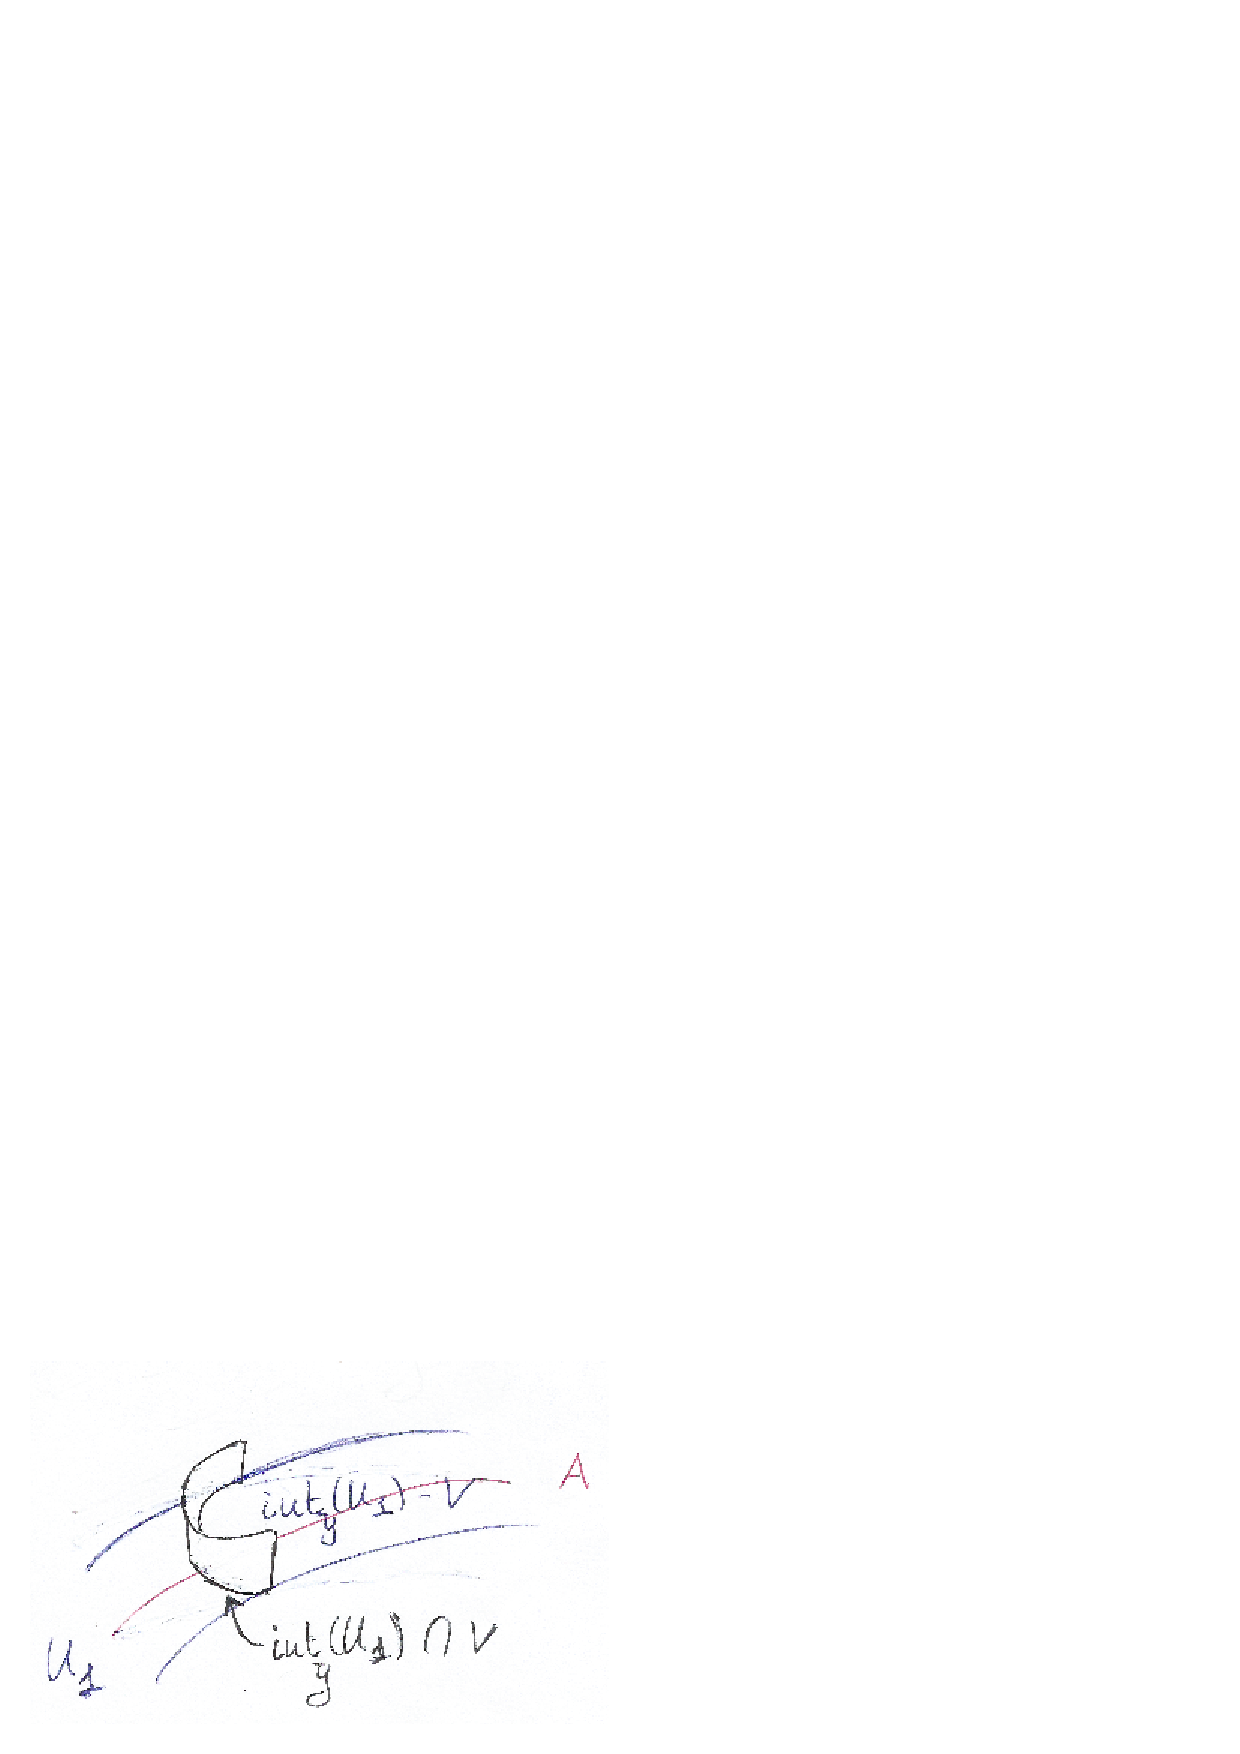
\includegraphics{Figures/ECompacto2.pdf}
\caption{\labfig{ECompacto2} Podemos retraer $V$ (superficies arqueadas) en
$U_1$ (banda plana) y $U_1$ en $A$ (línea discontinua).}
\end{subfigure}
\caption{Pasos ilustrados de la demostración.}
\end{marginfigure}

Ya sabemos que $U_1 \cup V$ se puede retraer en $A$. Dado que es unión de
compactos, es trivialmente compacto, de forma que habremos terminado la
demostración si podemos probar que $U_1 \cup V$ es entorno en $X$ de $A$.

Sea $y \in \Int_Y(U_1)$. Si $y \not\in V$, $y \in \Int_X(U_1)$
(repersentado como una banda en la ilustración \ref{ECompacto2}), por lo que
también estará en $\Int_X(U_1 \cup V)$.

Si $y \in V$, se tiene que $y \in \overline{D^m_i}\backslash D^m_i=
\phi(D^m\backslash \p D^m)=f(S^{m-1})$. Por otro lado,
$\phi^{-1}(\Int_Y(U_1))$ es un abierto de $S^{m-1}$ que contiene a
$\phi^{-1}(y)$ (por cómo se define $V$), de forma que 
\[\phi^{-1}(y) \in \Int_{S^{m-1}}\phi^{-1}(V) \implies y \in
\Int_{\overline{D^m_i}}(V)\]
Dado que $D^m_i$ es una célula de $X$, se sigue que $y \in
\Int_X(U_1\cup V)$.

Como $U_1$ es un entorno de $A$ en $Y$,
\[A \subseteq \Int_Y(U_1)\subseteq \Int_X(U_1\cup V)\]
por lo que $U_1\cup V$ es entorno de $A$ en $X$. Pero eso es lo que nos
quedaba por demostrar.
\end{proof}

\section{Grupos de homología celular}
\begin{corollary}\label{HomoCelular}
Si $X$ es un CW-complejo finito y $X^k$ es el $k$-esqueleto de $X$,
\[H_j(X^k,X^{k-1})=0 \quad \forall j \neq k\]
Además, $H_k(X^k,X^{k-1})$ es un grupo abeliano libre con un generador por
cada $k$-célula de $X$, conocido como el \textbf{grupo de homología celular}
de orden $k$.
\end{corollary}

\begin{proof}
Sabemos que $X^{k-1}$ es un subcomplejo de $X^k$. Por la proposición anterior,
existe un entorno compacto $U \subseteq X^k$ de $X^{k-1}$ tal que $X^{k-1}$
es un retracto por deformación fuerte de $U$.

Como $X$ es un CW-complejo finito, podemos hallar un homeomorfismo relativo
\[\phi: (\mc{D}^k, \mc{S}^{k-1}) \longrightarrow (X^k,X^{k-1})\]
utilizando los homeomorfismos $h$ que nos proporciona el teorema de
caracterización de CW-complejos finitos. Aplicando el teorema del
homeomorfismo relativo, se sigue que 
\begin{align*}
H_*(X^k,X^{k-1}) &\cong H_*(\mc{D}^k,\mc{S}^{k-1}) \cong 
	\sum^r_{i=1} H_*(D_i^k, S_i^{k-1}) \\
	& \cong \sum^r_{i=1} \tilde{H}_*(S^k) \cong
	\tilde{H}_*(S^k)^r \cong
	\begin{cases}
	\mb{Z}^r&\text{ si }p=k\\
	0&\text{ si no}
	\end{cases}
\end{align*}
\end{proof}

\begin{example}
Vamos a calcular la homología de la rosa de $p$ pétalos utilizando los grupos
de homología celular. Por la proposición \refprop{HomoCW},
\[H_j(B_p)\cong H_j(\{\star\})=0\]
para todo $j > 1$. Para $j=1$,
\[H_1(B_p)\cong \tilde{H}_1(B_p)\cong H_1(B_p,\{\star\})\]
Dado que $\{\star\}$ es el $0$-esqueleto de $B_p$, que tiene $p$ $1$-células, se
tiene que dicho grupo es isomorfo a $\mb{Z}^p$.
\end{example}

\section{Homología de la $n$-rosa}
Para $j=1,\dots,p$, sea $f_j\colon \p D^n \to \{\star\}$ la aplicación
constante. Se define la $n$-rosa de $p$ pétalos como la adjunción
\[X=B^n_p=\{\star\}_{f_1,\dots,f_p}\]

Por el corolario \ref{HomoCelular}, sabemos que $H_n(X^n,X^{n-1})\cong 
\mb{Z}^p$ y\\ $H_m(X^n,X^{n-1})=0$ para todo $m\neq n,0$. Sin embargo, $X^{n-1}
=X^0=\{\star\}$, por lo que
\begin{align*}
\mb{Z}^p\cong H_n(X,X^{n-1})=\tilde H_n(X);\\
0=H_m(X,X^{n-1})=\tilde H_m(X); && (m\neq n)
\end{align*}

\begin{theorem}\labthm{nrosa}
\[\tilde H_m(B^n_p)\cong
\begin{cases}
\mb{Z}^p & \text{si $m=n$}\\
0 & \text{si $m\neq n$}
\end{cases}\]
\end{theorem}

Al igual que pasaba con la $1$-rosa, cada pétalo que adjuntamos aporta un nuevo
generador, sólo que en este caso es la clase de un $n$-símplice singular.

\subsection{Rosa mixta}
¿Qué pasaría si mezcláramos pétalos de diferentes dimensiones? Intuitivamente,
cada pétalo de dimensión $k$ debería añadir un generador de orden $k$.

Sea $\alpha=(\alpha_1,\dots,\alpha_n) \in \mb{N}^n$. Si $f\colon \{\star\} \to
\{\star\}$ es la identidad, definimos
\[B_\alpha:=\{\star\}\cup_f B^1_{\alpha_1}\cup_f B^2_{\alpha_2}\cup_f \dots
\cup_f B^n_{\alpha_n}\]
siendo $B^k_0=\{\star\}$.

\begin{marginfigure}
\includegraphics{Figures/B22.png}
\caption{Ejemplo de rosa mixta $B_{(2,2)}$.}
\end{marginfigure}

\begin{theorem}\footnote{Este resultado está basado en una conversación que
tuve con mi directora del TFG, pero no pensé en añadirlo en su momento.}
\labthm{RosaMixta}
Dado $\alpha \in \mb{N}^n$,
\[H_m(B_\alpha)\cong
\begin{cases}
\mb{Z}			& \text{si $m=0$}\\
\mb{Z}^{\alpha_i} 	& \text{si $m=i$}\\
0				& \text{si $m > n$}
\end{cases}\]
\end{theorem}

\marginnote[-2.2cm]{
\begin{kaobox}[frametitle=Idea de la demostración]
\begin{itemize}
\item Probamos que la tesis se cumple cuando la rosa tiene $k_1$ pétalos de
dimensión $1$ (ya lo hemos hecho).
\item Suponemos que la tesis se cumple cuando la rosa tiene $k_1$ pétalos de
dimensión $1$, $k_2$ pétalos de dimensión $2$, y así hasta dimensión $n-1$.
\item Probamos que, como consecuencia, la tesis se cumple cuando añadimos $k_n$
pétalos de dimensión $n$.
\end{itemize}

Esta prueba puede ser conceptualmente engorrosa, así que es recomendable tratar
de hacer primero ejemplos para $n=2,3,4$.
\end{kaobox}
}

\begin{proof}
Si $\alpha=(\alpha_1,\dots,\alpha_n)$, procedemos por inducción sobre $n$. Si
$n=1$, $B_\alpha$ es una $1$-rosa de $\alpha_1$ pétalos, y la tesis se cumple
por \refthm{nrosa}.

Sea $\alpha'=(\alpha_1,\dots,\alpha_{n-1})$, y $X=B_{\alpha'}$. Supongamos que
la tesis se cumple para $X$ y sean $f_i\colon S^{n-1} \longrightarrow \{\star\}$
aplicaciones constantes. Tenemos entonces que
\[B_\alpha=X_{f_1\dots f_{\alpha_n}}\]

Por la \refprop{HomoCW}, si $(f_i)_*\colon \tilde H_{n-1}(S^{n-1})\to
H_{n-1}(\{\star\})=\{0\}$, se cumple lo siguiente:
\begin{enumerate}
\item Para todo $p\neq n,n-1$,
\[H_p(X_{f_1\dots f_{\alpha_n}})=H_p(X)\]
Por hipótesis de inducción, $H_p(X)\cong \mb{Z}^{\alpha_p}$ cuando $p < n-1$ y
$\{0\}$ cuando $p > n-1$.
\item Como $(f_i)_*$ va a parar a $\{0\}$ para todo $i$, $\im (f_i)_*=\{0\}$ y
\begin{align*}
H_{n-1}(X_{f_1\dots f_{\alpha_n}})&\cong
	\frac{H_{n-1}(X_{f_1\dots f_{\alpha_n-1}})}{\im (f_{\alpha_n})_*}\cong
	H_{n-1}(X_{f_1\dots f_{\alpha_n-1}})\cong\\
	&\cong \frac{H_{n-1}(X_{f_1\dots f_{\alpha_n-2}})}{\im (f_{\alpha_n-1})_*}\cong
	H_{n-1}(X_{f_1\dots f_{\alpha_n-2}})\cong\\
	&\cong \dots \cong H_{n-1}(X)
\end{align*}
Por hipótesis de inducción una vez más, ésto es $\mb{Z}^{\alpha_{n-1}}$.
\end{enumerate}

El tercer ítem requiere que hagamos inducción sobre el número de pétalos de
dimensión $n$\footnote{Al principio, pensé que era necesario tratar este
resultado como una \emph{doble inducción}, así que decidí leer sobre el tema.
Si bien he conseguido reducirlo a una inducción aislada dentro de otra, creo
que es un tema interesante, así que he decidido escribir un pequeño apéndice
sobre el tema.}. Dado un espacio $Y$ arbitrario, sabemos por la
\refprop{HomoCW} que la secuencia
\[0 \longrightarrow H_n(Y) \longrightarrow H_n(Y_{f})
\longrightarrow \ker f_*\longrightarrow 0\]
es exacta. En particular, $\ker f_*=\tilde H_{n-1}(S^{n-1})\cong \mb{Z}$ por el
\labthm{HRelSn}, por lo que
\begin{equation}
\mb{Z}\cong \frac{H_n(Y_f)}{H_n(Y)} \label{ExactaZ}
\end{equation}
En este caso, $H_n(X)=\{0\}$ por hipótesis de inducción, por lo que
$H_n(X_{f_1})\cong \mb{Z}$.

Supongamos que $H_n(X_{f_1\dots f_{\alpha_n-1}})\cong \mb{Z}^{\alpha_n-1}$.
Usando \eqref{ExactaZ}, concluimos que
\[H_n(X_{f_1\dots f_{\alpha_n}})\cong H_n(X_{f_1\dots f_{\alpha_n-1}})\oplus
\mb{Z}\cong \mb{Z}^{\alpha_n}\]
concluyendo así ambas inducciones. Se sigue la tesis.
\end{proof}

\input{chapters/Superficies}
%\setchapterpreamble[u]{\margintoc}

\chapter{Cohomología singular}

\section{Grupos de cohomología}
\begin{definition}
Un complejo de cocadenas es un par $(C,d)$ donde $C=\{C^j: j \in \mb{Z}\}$ es
un grupo abeliano graduado y $d\colon C \to C$ es un endomorfismo graduado
de grado $1$ tal que $d^{p+1}\circ d^p=0$. Es decir, tenemos una sucesión
exacta
\[0 \longrightarrow C^0 \xrightarrow{d^0} C^1 \xrightarrow{d^1} C^2
\xrightarrow{d^2}\dots\]
donde las flechas van hacia arriba, en lugar de ir hacia abajo.
\end{definition}

En este capítulo, veremos que muchos términos de homología singular se
repiten, añadiendo el prefijo \emph{co-}. Ésto se debe a que la teoría de
cohomología complementa a teoría de homología, dado que estamos utilizando
los mismos principios, pero aquí le damos la vuelta al sentido de las flechas
en las sucesiones exactas.

Al igual que hay diferentes teorías de homología (simplicial, singular,
celular...), existen diferentes teorías de cohomología que están diseñadas
para diferentes contextos. En este capítulo, cubriremos la teoría de
cohomología singular, que es la más general y no requiere ningún conocimiento
preeliminar que no hayamos visto ya.

Los elementos de $C^n$ se denominan \textbf{cocadenas} de orden $n$, y los
homomorfismos $d^n$ reciben el nombre de \textbf{operadores coborde}.

\marginnote[-2.2cm]{
\begin{kaobox}[frametitle=Coborde y cobordismo]
El \emph{coborde} que definimos en este capítulo no está relacionado con
los \emph{cobordismos}. Sin entrar en detalles, se podría decir que dos
variedades $X$ e $Y$ de dimensión $n$ son cobordantes si existe una
homotopía
\[F\colon X \simeq Y\]
cuyo grafo es una variedad con bordes de dimensión $n+1$.
\end{kaobox}
}

Definimos el grupo de $n$-cociclos como $Z^n(C)=\ker d^n$, y el grupo de $n$-
cobordes como $B^n(C)=\im d^n$. Dado que $d^{n+1}\circ d^n=0$, $B^n(C)\leq
Z^n(C)$, por lo que definimos el \textbf{grupo $n$-ésimo de cohomología} como
\[H^n(C)=\frac{Z^n(C)}{B^n(C)}\]
Notar que, para diferenciar los grupos usados en teoría de homología de los
usados en teoría de cohomología, convertimos los subíndices en superíndices.

\begin{definition}
Dados dos complejos de cocadenas $(C,d)$ y $(D,d')$, una \textbf{aplicación
de cocadenas} es un homomorfismo graduado $f\colon C \to D$ que conmuta con
el operador coborde (i.e. $d'\circ f=f\circ d$).
\end{definition}

Una aplicación de cocadenas $f$ siempre induce un homomorfismo en
cohomología,
\begin{diag}
f^*\colon H^*(C)\arrow[r] &H^*(D)\\[-8mm]
\left[c\right] \arrow[r,maps to]& \left[f(c)\right]
\end{diag}

\subsection{Cohomología singular}

\marginnote[-2.2cm]{
\begin{kaobox}[frametitle=Anillos]
Tanto la teoría de homología como cohomología se puede construir utilizando
anillos que no sean $\mb{Z}$; sin embargo, es más común encontrar casos
donde la cohomología se calcula para diferentes anillos (como nuestra
principal referencia, \cite{Vick94}).
\end{kaobox}
}

Sea $X$ un espacio topológico y $S_*(X)$ el grupo de cadenas singulares de
$X$. Dado un $n \in \mb{Z}$ y un anillo $R$, definimos el grupo de cocadenas
singulares $S^n(X;R)$ como el grupo formado por todos los homomorfismos de
la forma $\phi\colon S_n(X) \to R$.

\begin{theorem}
Sea $X$ un espacio topológico y $\p$ el operador borde asociado a $S_*(X)$.
El homomorfismo graduado $d=\{d^n\colon n \in \mb{Z}\}$,
\begin{diag}
d^n\colon S^n(X;R)\arrow[r] &S^{n+1}(X;R)\\[-8mm]
\phi \arrow[r,maps to]& \phi\circ \p_n
\end{diag}
define un operador coborde. Por tanto, $(S^*(X;R),d)$ es un complejo de
cocadenas.
\end{theorem}

Dada una aplicación continua $f\colon X \to Y$, podemos considerar la
aplicación inducida en cocadenas,
\begin{diag}
f^\#\colon S^n(X;R)\arrow[r] &S^n(Y;R)\\[-8mm]
\phi \arrow[r,maps to]& \phi\circ f
\end{diag}
que induce a su vez un homomorfismo en cohomología, $f^*\colon H^*(Y;R) \to
H^*(X;R)$. Si bien esta aplicación se asemeja al \emph{pull-back} de
geometría diferencial, es importante notar que $f^*$ actúa sobre clases y
no aplicaciones.

\section{Productos en cohomología}
En ciertos contextos, las teorías de cohomología se consideran más poderosas
que las teorías de homología. Esto se debe entre otras cosas a que podemos
dotar a $H^*(X)$ de una estructura de anillo, mediante la cual podemos
separar espacios topológicos que los grupos de homología no pueden
distinguir.

Sean $p,q \geq 0$ y $\phi\colon \sigma_{p+q} \to X$ un símplice singular.
Definimos
\begin{align*}
\phi^{(p)}(t_0,\dots,t_p)=\phi(t_0,\dots,t_p,0,\dots,0);\\
\phi^({q})(t_0,\dots,t_q)=\phi(0,\dots,0,t_0,\dots,t_q)
\end{align*}

\begin{definition}
Sean $c \in S^p(X;R)$ y $d \in S^q(X)$. Se define el producto de $c$ y $d$
como la $(p+q)$-cocadena $c\smile d \in S^{p+q}(X;R)$ dada por
\[(c\smile d)(\phi):=c(\phi^{(p)})d(\phi_{(q)})\]
La ley de composición interna $\smile$ recibe el nombre de \textbf{operador
copa}, e induce una estructura de anillo en $H^*(X;R)$.
\end{definition}

\subsection{Dualidad de Poincaré}
\begin{theorem}
Sea $M$ una variedad sin borde, compacta, conexa y orientable de dimensión
$n$. Si $s\colon M \to T$ es una orientación y $z$ es la
clase fundamental asociada a $M$, el homomorfismo
\begin{diag}
D\colon H^k(M;R)\arrow[r] &H_{n-k}(M;R)\\[-8mm]
\left[x\right] \arrow[r,maps to]& \left[x\frown z\right]
\end{diag}
es un isomorfismo para todo $k$.
\end{theorem}

\begin{example}[\cite{MSE}]
Sean $X=S^2\times S^2$ e $Y$ la suma conexa de dos copias de $\mb{CP}^2$.
Por un lado, tenemos que $H_*(X)\cong H_*(Y)$. Sin embargo,
\begin{align*}
H^*(X;\mb{Z})\cong \frac{\mb{Z}[x,y]}{(x^2,y^2)}; &&
H^*(Y;\mb{Z})\cong \frac{\mb{Z}[x,y]}{(x^3,y^3,xy)}
\end{align*}
que son anillos diferentes.
\end{example}

%\input{chapters/figsntabs.tex}
%\input{chapters/references.tex}

%\input{chapters/layout.tex}
%\input{chapters/mathematics.tex}

\appendix % From here onwards, chapters are numbered with letters, as is the appendix convention
\chapter{Método de doble inducción}\label{DobleInd}
El propósito de este apéndice es explicar en detalle cómo funciona la
\emph{doble inducción} utilizada en la demostración del \refthm{RosaMixta},
por qué es un método de demostración válido (cuando se usa correctamente) y
bajo qué condiciones podemos hacer \emph{inducción múltiple}.

\begin{definition}
Sea $(S,<)$ un conjunto totalmente ordenado. Dado $s \in S$, definimos el
\textbf{sucesor} de $s$ como el menor $s' \in S$ tal que $s < s'$. El sucesor
está bien definido porque el orden es total.
\end{definition}

\marginnote[-2.2cm]{
\begin{kaobox}[frametitle=Conjunto bien ordenado]
Un conjunto totalmente ordenado $(S,<)$ está bien ordenado si, dado un
subconjunto $S' \subset S$, $S'$ tiene un elemento minimal. Por ejemplo,
$\mb{N}$ está bien ordenado, pero $\mb{Z}$ no.

Un ejemplo de subconjunto que no cumple esta propiedad es el conjunto de los
enteros negativos.
\end{kaobox}
}

Si $P(n)$ es una propiedad que depende de $n \in \mb{N}$, el método de
inducción matemática se puede representar como un diagrama de la forma
\begin{diag}
P(1) \arrow[r] & P(2) \arrow[r] & \dots \arrow[r] & P(n) \arrow[r] & \dots
\end{diag}
Este método se basa en el hecho de que $\mb{N}$ es un conjunto bien ordenado
bajo la relación $\leq$ (i.e. todo conjunto no vacío de números naturales tiene
un mínimo). En general, podemos plantear un método de inducción sobre cualquier
conjunto totalmente ordenado.

\begin{definition}
Sea $(S,<)$ un conjunto totalmente ordenado. Supongamos que, dada una propiedad
$P(s)$ que depende de $s \in S$, tenemos los siguientes resultados:
\begin{enumerate}
\item $P(\min\{s\})$ es cierto;
\item si $s'$ es el sucesor de $s$, $P(s)$ implica $P(s')$.
\end{enumerate}
Diremos que $S$ admite un método de inducción si estas dos propiedades implican
que $P(s)$ es cierto para todo $s \in S$.
\end{definition}

\begin{proposition}[\cite{BienOrd}]
Sea $S$ un conjunto totalmente ordenado. El conjunto $S$ admite un método de
inducción si y sólo si está bien ordenado.
\end{proposition}

Consideremos entonces el caso de una propiedad $Q(n,m)$ que depende de $n,m \in
\mb{N}$. En este caso, nuestro conjunto de partida es $\mb{N}^2$, así que
necesitamos una relación de orden total para poder probar $Q$ por inducción.

Dados $(n_1,m_1),(n_2,m_2) \in \mb{N}$, definimos el orden lexicográfico
$\prec$ como
\[(n_1,m_1) \prec (n_2,m_2) \iff
\begin{cases}
n_1 < n_2\\
n_1 = n_2; & m_1 < m_2
\end{cases}
\]
El orden lexicográfico se puede extender a $\mb{N}^k$, y se utiliza en algunos
campos del álgebra tales como la teoría de polinomios. Dado que el orden
lexicográfico es el orden usual de $\mb{N}$ \emph{aplicado dos veces}, es fácil
ver que induce un buen orden en $\mb{N}^2$, por lo que podemos probar $Q$ de
forma inductiva.

Para poder probar $Q$, lo que tenemos que hacer es probar primero $P(n)=Q(n,1)$
por inducción sobre $n$, y después, probar $R(m)=Q(n,m)$ por inducción sobre
$m$. El diagrama correspondiente toma la forma
\begin{diag}
Q(1,1) \arrow[r] \arrow[d, dashed] & Q(2,1) \arrow[r] \arrow[d,dashed] &
	\dots \arrow[r] \arrow[d,dashed] & Q(n,1) \arrow[r] \arrow[d,dashed] &
	 \dots \arrow[d,dashed]\\
Q(1,2) \arrow[r] \arrow[d, dashed] & Q(2,2) \arrow[r] \arrow[d,dashed] &
	\dots \arrow[r] \arrow[d,dashed] & Q(n,2) \arrow[r] \arrow[d,dashed] &
	\dots \arrow[d,dashed]\\
\vdots \arrow[r] \arrow[d, dashed] & \vdots \arrow[r] \arrow[d,dashed] &
	\ddots \arrow[r] \arrow[d,dashed] & \vdots \arrow[r] \arrow[d,dashed] &
	\vdots \arrow[d,dashed]\\
Q(1,m) \arrow[r] \arrow[d, dashed] & Q(2,m) \arrow[r] \arrow[d,dashed] &
	\dots \arrow[r] \arrow[d,dashed] & Q(n,m) \arrow[r] \arrow[d,dashed] &
	\dots \arrow[d,dashed]\\
\vdots \arrow[r] & \vdots \arrow[r] & \vdots \arrow[r] & \vdots \arrow[r] &
	\dots
\end{diag}
donde las líneas sólidas representan $n_1 < n_2$, y las líneas discontinuas,
$m_1 < m_2$.
\setchapterpreamble[u]{\margintoc}

\chapter{Complementos}
\section{Complementos de la parte 1}
\subsection{Teorema del punto fijo de Brouwer}
Uno de los resultados clásicos de la topología algebraica es el
\textbf{teorema del punto fijo de Brouwer}, de gran importancia en diversas
áreas de las matemáticas tales como la teoría de juegos. La formulación
estándar del teorema de Brouwer (así como la de otros muchos teoremas de punto
fijo de análisis funcional) es la siguiente:

\begin{theorem}[Teorema del punto fijo de Brouwer]
Sea $D$ una bola cerrada y  $f: D^n \to D^n$ una función continua. Existe un
$p \in D$ tal que $f(p)=p$.
\end{theorem}

\begin{proof}
Supongamos que $f$ no posee puntos fijos:
\[\forall x\in D^n \quad f(x)\neq x \iff \|x-f(x)\| > 0\]
Consideramos entonces la semirrecta
\begin{align*}
r_x=\{\mu u(x)+x: \mu \geq 0\}; && u(x)=\frac{x-f(x)}{\|x-f(x)\|}
\end{align*}
Se define la correspondencia $g\colon D \to \p D$ que asigna a $x$ un
punto $g(x)\in r_x\cap \p D$.

\begin{marginfigure}
\resizebox{\textwidth}{!}{
\begin{tikzpicture}
\draw (0,0) circle (2cm);				

\draw[-to] (.8,.8) -- (-2,-2);
\draw[fill=green] (.8,.8) circle (2pt);
\draw[fill=green] (-.4,-.4) circle (2pt);
\draw[fill=green] (-1.42,-1.42) circle (2pt);

\draw[stealth-stealth] (-3,0) -- (3,0);
\draw[stealth-stealth] (0,-3) -- (0,3);
	
\draw (1.2,.6) node {$f(x)$};
\draw (-.4,-.8) node {$x$};
\draw (-2,-1.42) node {$g(x)$};
\end{tikzpicture}
}
\caption[Aplicación $g$ ilustrada.]{La aplicación $g$ extiende una semirrecta
que pasa por los puntos $x$ y $f(x)$ para tomar el punto de intersección
con la esfera unidad. Dicho punto de intersección es $g(x)$.}
\end{marginfigure}

Queremos ver que $g(x)$ es un singulete. Dados dos puntos $p,q \in r_x$,
existen $\lambda, \mu \geq 0$ tales que
\[p=u_x\mu+x; \quad q=u(x)\lambda+x \implies p-q=u(x)(\mu-\lambda)\]
Tomando normas a ambos lados de la igualdad,
\[\|p-q\|=|\mu-\lambda|\|u(x)\|=|\mu-\lambda|\]
de lo que se deduce que no hay dos puntos diferentes con la misma norma. Por
tanto, $g$ es una aplicación continua.

Observar que, si $x \in \p D$, será el único punto de $r_x$ con norma $1$.
De aquí se sigue que $g$ fija los puntos de $\p D$, por lo que es un retracto
fuerte e induce un epimorfismo
\[g_*\colon H_n(D) \longrightarrow H_n(\p D)\]

Como $D$ es convexo, $H_n(D)$ es un grupo trivial para todo $n > 0$; no
obstante, $\p D$ es homeomorfo a un cierto $S^n$, por lo que $H_n(\p D)$
tiene rango 1. Dado que $g_*$ es sobreyectiva, si llamamos $\alpha$ al
generador de $H_n(\p D)$, existirá un $b \in H_n(\p S)$ tal que $f(b)=\alpha$.

Dado que $b \in H_n(D)=0$, se tiene que $\alpha=f(b)=0$, en contradicción
con el hecho de que $\alpha$ es un generador de un grupo no trivial. Por tanto,
existe un $x \in D$ tal que $f(x)=x$.
\end{proof}

\subsection{Grado de Brouwer}
Sean $n \geq 1$ y $f\colon S^n \to S^n$ una aplicación continua no nula. Dado
un generador $\alpha \in H_n(S^n)$, $f_*(\alpha)=m\alpha$ para algún
$m\neq 0$. Este valor es independiente del $\alpha$ que hemos elegido, dado
que
\[f_*(-\alpha)=m(-\alpha)=-(m\alpha)=-f_*(\alpha)\]
por lo que podemos identificar $m$ con $f$. Este valor se denota como $d(f)$
\footnote{No confundir con la diferencial de una aplicación diferenciable.}
y se denomina \textbf{grado de Brouwer} de $f$.

El grado de Brouwer tiene las siguientes propiedades fundamentales:
\begin{enumerate}
\item Si $f$ es la identidad, $d(f)=1$.
\item Dados $S^n \xrightarrow{f} S^n \xrightarrow{g} S^n$, $d(f\circ g)=
d(f)d(g)$.
\item Si $f$ es constante, $d(f)=0$.
\item Dados $S^n \xrightarrow{f} S^n \xrightarrow{g} S^n$, $f$ es homotópica
a $g$ si y sólo si $d(f)=d(g)$.
\item La aplicación $f$ es una equivalencia de homotopía si y sólo si $d(f)$
es $\pm 1$.
\end{enumerate}

Dada una apliación $f\colon S^n \to S^n$, consideramos la aplicación
$\Sigma f\colon S^{n+1}\to S^{n+1}$ dada por
\[\Sigma f(x,t)=
\begin{cases}
(0,t)				& \text{if $x=0$}\\
(\|x\|f(x/\|x\|),t)	& \text{if $x\neq 0$}
\end{cases}\]
donde $(x,t) \in \mb{R}^{n+1}\times\mb{R}$ verifica que $\|x\|^2+|t|=1$. Esta
aplicación se denomina \textbf{suspensión} de $f$.

\begin{proposition}
Si $f\colon S^n \to S^n$ verifica que $n > 0$, $d(\Sigma f)=d(f)$.
\end{proposition}

Para poder visualizar la suspensión de $f$, consideramos $S^n$ como el ecuador
de $S^{n+1}$. Dado un $t \in [-1,1]$, si $S_t^n$ es el subespacio de $S^{n+1}$
dado por $x_{n+2}=t$, la aplicación
\begin{diag}
\phi_t\colon S^n \arrow[r] & S^n_t\\[-8mm]
			x \arrow[maps to,r] &(\left[1-t\right]x,t)
\end{diag}
es un homeomorfismo y verifica que
\[\Sigma f|_{S^n_t}=\phi_t\circ f\circ \phi_t^{-1}\]

\begin{proposition}
Sean $n > 0$ y $f\colon S^n \to S^n$ la aplicación
\[f(x_1,\dots,x_{n+1})=(-x_1,x_2,\dots,x_{n+1})\]
Entonces, $d(f)=-1$.
\end{proposition}

\begin{proof}
Consideremos el caso $n=1$. Sean $N=(0,1)$, $S=(0,-1)$ y $W=(-1,0)$,
$E=(1,0)$. Entonces, $f$ es Mayer-Vietoris continua bajo el recubrimiento
$U=S^1\backslash \{S\}$, $V=S^1\backslash \{N\}$.

Sea $f_3=f|_{U\cap V}$. El diagrama
\begin{diag}
0 \arrow[r] & H_1(S^1) \arrow{r}{\Delta} \arrow{d}{f_*} & H_0(U\cap V)
	\arrow{d}{f_{3*}}\\
0 \arrow[r] & H_1(S^1) \arrow{r}{\Delta} & H_0(U\cap V)
\end{diag}
tiene filas exactas, y el rectángulo es conmutativo. Un generador $\alpha$ de
$H_1(S^1)$ se puede representar como un ciclo en la forma $c+d$, donde
$\p c=x-y=-\p d$, en cuyo caso $\Delta(\alpha)=x-y$. Ahora bien,
\[(\Delta\circ f_*)(\alpha)=(f_{3*}\circ \Delta)(x)=f_{3*}(x-y)=y-x=
-\Delta(\alpha)=\Delta(-\alpha)\]
Dado que $\Delta$ es un monomorfismo, $d(f)=-1$.

Asumamos ahora que $d(f)=-1$ para $n-1 \geq 1$. Consideramos $S^{n-1}$ como el
subespacio de $S^n$ dado por la ecuación $x_{n+1}=0$, de forma que $S^{n-1}$ es
el ecuador de $S^n$. Tomamos $U=S^n\backslash \{N\}$ y $V=S^n\backslash \{S\}$,
siendo $N=(0,\dots,0,1)$ y $S=(0,\dots,0,-1)$. Con esta notación, la inclusión
\[i\colon S^{n-1}\hookrightarrow U\cap V\]
es una equivalencia de homotopía.

Dado que $n > 1$, el homomorfismo de conexión $\Delta$ es un homomorfismo. Por
tanto, tenemos el doble diagrama conmutativo
\begin{diag}
H_n(S^n) \arrow{r}{\Delta} \arrow{d}{f_*} & H_{n-1}(U\cap V)
	\arrow{d}{f_{3*}} & H_{n-1}(S^{n-1}) \arrow[swap]{l}{i_*} \arrow{d}{f_*}\\
H_n(S^n) \arrow{r}{\Delta} & H_{n-1}(U\cap V) & H_{n-1}(S^{n-1})
	\arrow[swap]{l}{i_*}
\end{diag}
donde las filas describen isomorfismos. Si llamamos $\alpha$ al generador de
$H_n(S^n)$,
\begin{align*}
f_*(\alpha)&=(\Delta^{-1}\circ f_{3*}\circ \Delta)(\alpha)
=(\Delta^{-1}\circ i_*\circ f_{3*}\circ i_*^{-1}\circ \Delta)(\alpha)=\\
&=-(\Delta^{-1}\circ i_*\circ i_*^{-1}\circ \Delta)(\alpha)=-\alpha
\end{align*}
\end{proof}

Como consecuencia de este resultado, si $f$ cambia el signo de $1 \leq j\leq
n$ componentes, $d(f)=(-1)^j$. En particular, la aplicación antipodal
$A(x)=-x$ tiene grado de Brouwer $(-1)^n$.

\begin{proposition}\labprop{Antipodal}
Si $f,g\colon S^n \to S^n$ son aplicaciones con $f(x)\neq g(x)$ para todo $x$,
$g$ es homotópica a $A\circ f$.
\end{proposition}

\begin{proof}
Dado que $f(x)\neq g(x)$, el segmento
\[L=\{tA[f(x)]+(1-t)g(x)\colon t \in [0,1]\}\]
no contiene al punto $0$. Por tanto, la homotopía $F\colon S^n\times I \to
S^n$ dada por
\[F(x,t)=\frac{tA[f(x)]+(1-t)g(x)}{\|tA[f(x)]+(1-t)g(x)\|}\]
está bien definida.
\end{proof}

\begin{marginfigure}
\resizebox{\textwidth}{!}{
\begin{tikzpicture}
	\draw (2,0) -- (0,2);
	\draw[dashed] (0,0) circle (2cm);
	\draw (0.7,0.7) node {$L$};
	
	\draw[fill=green] (2,0) circle (1pt);
	\draw (2.5,0) node {$g(x)$};

	\draw[fill=green] (0,2) circle (1pt);
	\draw (0,2.5) node {$A[f(x)]$};

	\draw[fill=green] (0,-2) circle (1pt);
	\draw (0,-2.5) node {$f(x)$};
	
	\draw[thick] (2,0) arc (0:90:2cm);
	\draw (1.8,1.8) node {$F(L\times I)$};

\end{tikzpicture}
}

\caption{Representación gráfica de la \refprop{Antipodal}.}
\end{marginfigure}

Consideremos una $f\colon S^{2n} \to S^{2n}$ continua. Si $f(x)\neq x$ para
todo $x$, $f$ es homotópica a $A=A\circ \id_{S^{2n}}$ y
\[d(f)=d(A)=(-1)^{2n+1}\]
Si suponemos que $f(x)\neq -x$ para todo $x$, $f$ es homotópica a
$\id_{S^{2n}}=A\circ A$ y
\[d(f)=d(\id)=1\]
Dado que $d(f)$ es único, debe pasar que $f(x)=x$ ó $f(x)=-x$ para algún
$x \in S^{2n}$.

\begin{corollary}[Teorema de la bola peluda]
Dada $f\colon S^{2n} \to S^{2n}$ continua, $f(x)$ no puede ser ortogonal a $x$
para todo $x$. Por tanto, todo campo vectorial sobre $S^{2n}$ es nulo.
\end{corollary}

\section{Complementos de la parte 2}


%----------------------------------------------------------------------------------------

\backmatter % Denotes the end of the main document content
\setchapterstyle{plain} % Output plain chapters from this point onwards

%----------------------------------------------------------------------------------------
%	BIBLIOGRAPHY
%----------------------------------------------------------------------------------------

% The bibliography needs to be compiled with biber using your LaTeX editor, or on the command line with 'biber main' from the template directory

\defbibnote{bibnote}{Here are the references in citation order.\par\bigskip} % Prepend this text to the bibliography
%\printbibliography[heading=bibintoc, title=Bibliography, prenote=bibnote] % Add the bibliography heading to the ToC, set the title of the bibliography and output the bibliography note

%	\bibliographystyle{plain}
%	\input{chapters/Referencias.bbl} 

%----------------------------------------------------------------------------------------
%	NOMENCLATURE
%----------------------------------------------------------------------------------------

% The nomenclature needs to be compiled on the command line with 'makeindex main.nlo -s nomencl.ist -o main.nls' from the template directory

%\nomenclature{$c$}{Speed of light in a vacuum inertial frame}
%\nomenclature{$h$}{Planck constant}

%\renewcommand{\nomname}{Notation} % Rename the default 'Nomenclature'
%\renewcommand{\nompreamble}{The next list describes several symbols that will be later used within the body of the document.} % Prepend this text to the nomenclature

%\printnomenclature % Output the nomenclature

%----------------------------------------------------------------------------------------
%	INDEX
%----------------------------------------------------------------------------------------

% The index needs to be compiled on the command line with 'makeindex main' from the template directory

%\printindex % Output the index

%----------------------------------------------------------------------------------------
%	BACK COVER
%----------------------------------------------------------------------------------------

% If you have a PDF/image file that you want to use as a back cover, uncomment the following lines

%\clearpage
%\thispagestyle{empty}
%\null%
%\clearpage
%\includepdf{cover-back.pdf}

%----------------------------------------------------------------------------------------

\end{document}
